%%%%%%%%%%%%%%%%%%%%%%%%%%%%%%%%%%%%%%%%%%%%%%%%%%%%%%%%%%%%%%%%%%%%%%%%%%
%%%%%                         CHAPITRE 4                            %%%%%%
%%%%%%%%%%%%%%%%%%%%%%%%%%%%%%%%%%%%%%%%%%%%%%%%%%%%%%%%%%%%%%%%%%%%%%%%%%

\lhead[\fancyplain{}{\leftmark}]%Pour les pages paires \bfseries
      {\fancyplain{}{}} %Pour les pages impaires
\chead[\fancyplain{}{}]%
      {\fancyplain{}{}}
\rhead[\fancyplain{}{}]%Pour les pages paires 
      {\fancyplain{}{\rightmark}}%Pour les pages impaires \bfseries
\lfoot[\fancyplain{}{}]%
      {\fancyplain{}{}}
\cfoot[\fancyplain{}{\thepage}]%\bfseries
      {\fancyplain{}{\thepage}} %\bfseries
\rfoot[\fancyplain{}{}]%
     {\fancyplain{}{\scriptsize}}


%%%%%%%%%%%%%%%%%%%%%%%%%%%%%%%%%%%%%%%%%%%%%%%%%%%%%%%%%%%%%%%%%%%%%%%%%%
%%%%%                      Start part here                          %%%%%%
%%%%%%%%%%%%%%%%%%%%%%%%%%%%%%%%%%%%%%%%%%%%%%%%%%%%%%%%%%%%%%%%%%%%%%%%%%

\chapter{Modélisation de la notion de qualité par apprentissage}
\label{ch:metric_learning}

% Epigraphe
%PSYCHOHISTOIRE : Gaal Dornick a défini la
%psychohistoire comme la branche des mathématiques qui traite
%des réactions des ensembles humains en face de phénomènes
%sociaux et économiques constants...
%... Cette définition sous-entend que l'ensemble humain en
%question est assez important pour qu'on puisse valablement lui
%appliquer la méthode statistique. L'importance numérique
%minimale de cet ensemble peut être déterminée par le Premier
%Théorème de Seldon qui... Une autre condition nécessaire est
%que ledit ensemble humain ignore qu'il est soumis à l'analyse
%psychohistorique, afin que ses réactions n'en soient pas
%troublées...
%Toute psychohistoire valable repose sur les Fonctions de
%Seldon qui présentent des propriétés analogues à celles de
%forces économiques et sociales telles que...
%ENCYCLOPEDIA GALACTICA.
%
%
%- C'est assez. Et quelles sont les probabilités numériques de
%destruction totale d'ici cinq siècles ?
%– 17 –
%- Je ne saurais vous le dire.
%- Voyons, vous savez tout de même faire une différentiation
%de champ ? "
%Gaal se sentit pris de court. Seldon ne lui proposa pas son
%bloc à calcul ; il dut donc faire ses opérations de tête. La sueur
%se mit à couler de son front.
%" Environ 85 pour cent ? dit-il enfin.
%- Pas mal, dit Seldon, pas mal, mais ce n'est pas tout à fait
%cela. Le chiffre exact est 92,5 pour cent.
%- Voilà donc, dit Gaal, pourquoi on vous appelle Cassandre
%Seldon. Comment se fait-il que je n'aie jamais rien vu de tout
%cela dans les journaux ?
%- On ne peut pas publier des choses pareilles, voyons. Vous
%ne pensez tout de même pas que l'Empire irait révéler ainsi sa
%faiblesse. C'est une démonstration de psychohistoire
%élémentaire. Mais certains des résultats de nos calculs sont
%venus aux oreilles de l'aristocratie.


%“It’s always easy to explain the unknown by postulating a superhuman and arbitrary will.”
%― Isaac Asimov, Second Foundation
%
%
%“Now tell me what happened—in words. I want your translation of the mathematics.”
%― Isaac Asimov, Second Foundation

%============================================================================== Résumé du chapitre

\begin{center}
\rule{0.7\linewidth}{.5pt}
\begin{minipage}{0.7\linewidth}
\smallskip

\textit{
	Dans ce chapitre, nous étudierons les différentes méthodes de la littérature permettant de modéliser la notion de qualité par apprentissage statistique.
	L'objectif est de construire un modèle qui permet à partir d'images, d'inférer la qualité des pièces.
	Nous discuterons de l'optimisation de l'apprentissage de ces modèles.
	Le diagramme \ref{fig:deep_flowchart} synthétise cette démarche.
	C'est sous le prisme des contraintes industrielles que nous discuterons des limites au déploiement de ces méthodes sur les lignes de production.
}

%\smallskip
\end{minipage}
\smallskip
\rule{0.7\linewidth}{.5pt}
\end{center}

\minitoc

\newpage
\null
\vfill

\newcommand*{\h}{\hspace{2pt}}% for indentation
\newcommand*{\hh}{\h\h}% double indentation
\begin{figure}[hbtp]
    \centering
    \hspace*{8em}\begin{tikzpicture}[auto,
    %decision/.style={diamond, draw=black, thick, fill=white,
    %text width=8em, text badly centered,
    %inner sep=1pt, font=\sffamily\small},
    block_center/.style ={rectangle, draw=black, thick, fill=white,
        text width=17em, text centered,
        minimum height=3.5em},
    block_left/.style ={rectangle, draw=black, thick, fill=white,
        text width=16em, text ragged, minimum height=4em, inner sep=6pt},
    block_noborder/.style ={rectangle, draw=none, fill=none,
        text width=9em, text ragged, minimum height=2em, inner sep=0pt},
    block_assign/.style ={rectangle, draw=black, thick, fill=white,
        text width=18em, text ragged, minimum height=3em, inner sep=6pt},
    block_lost/.style ={rectangle, draw=black, thick, fill=white,
        text width=16em, text ragged, minimum height=3em, inner sep=6pt},
    line/.style ={draw, thick, -latex', shorten >=0pt},
    decoration=brace]
    \matrix [column sep=5mm,row sep=2em] {
        % row 1
        \node [block_center] (data_collection) {Acquisition de données représentatives};
        & \node [block_noborder] {Exploration des points de fonctionnement du procédé}; \\
        % row 2
        \node [block_center] (extraction) {Extraction de variables pertinentes}; 
        & \node [block_noborder] {Réduction de dimensions}; \\
        % row 3
        \node [block_center] (classification) {Construction et apprentissage du modèle};
        & \node [block_noborder] {Classification de la qualité}; \\
        % row 4
        \node [block_center] (validation) {Validation des performances};
        & \node [block_noborder] {Métriques des faux positifs/négatifs}; \\
        % row 5
        \node [block_center] (deployement) {Déploiement du modèle en production};
        & \node [block_noborder] {Classification de la conformité en sortie de machine}; \\
    };% end matrix
	\draw[decorate,transform canvas={xshift=-1em},thick,align=center] (data_collection.south west) -- node[left=2pt] {Mesure \\ en ligne §\ref{ch:dataset}} (data_collection.north west);
    \draw[decorate,transform canvas={xshift=-1em},thick,align=center] (classification.south west) -- node[left=2pt] {Deep \\ Learning \\ §\ref{sec:metric_learning}} (extraction.north west);
    \draw[decorate,transform canvas={xshift=-6em},thick,align=center] (validation.south west) -- node[left=2pt] {AutoML \\ §\ref{sec:auto_ml}} (extraction.north west);
    \draw[decorate,transform canvas={xshift=-11em},thick,align=center] (deployement.south west) -- node[left=2pt] {Contrôle \\ de la \\ qualité \\ par \\ apprentissage} (data_collection.north west);
    % connecting nodes with paths
    \begin{scope}[every path/.style=line]
    % paths for enrollemnt rows
    \path (data_collection)   -- (extraction);
    \path (extraction) -- (classification);
    \path (classification) -- (validation);
    \path (validation) -- (deployement);
    \end{scope}
    \end{tikzpicture}
    \caption{Diagramme du processus de construction d'un algorithme de contrôle de la qualité par apprentissage.}
    \label{fig:deep_flowchart}
\end{figure}

\vfill
\newpage

\section{Construction d'une métrique de la qualité par apprentissage} \label{sec:metric_learning}
La notion de qualité d'un produit est spécifiée dans le cahier des charges.
Cependant, lorsque les spécifications ne sont pas normées, elles entrainent souvent une traduction subjective.
C'est pourquoi la notion de qualité d'un produit, lorsqu'elle intègre les aspects sensoriels en plus des tolérances géométriques, est souvent subjective.
Elle s'appuie sur une connaissance holistique d'un expert qualité humain. La notion de qualité d'aspect est difficile à formaliser.
Des travaux de recherches ont permis des avancées dans ce domaine.
L'analyse ontologique de corpus de textes de références permet par exemple de hiérarchiser les descriptions formelles afin de normaliser ces notions de qualité du point de vue visuel \cite{baudet_maitrise_2012} et sensorimoteur \cite{albert_smart_2017}.
Une fois normée, le contrôle de la qualité peut être automatisé \cite{desage_contraintes_2015, pitard_metrologie_2016, lacombe_exploitation_2018a, albert_maitrise_2019} afin de garantir la répétabilité.

Construire une métrique de la qualité par apprentissage revient à apprendre la fonction $f_{\theta}$ qui a pour paramètres $\theta$ tel que $f_{\theta}(\mathbf{x}) : \mathbb{R}^{F} \rightarrow \mathbb{R}^{D}$ transforme les points de l'espace d'origine $\mathbb{R}^{F}$ dont les propriétés sont similaires (par exemple un niveau de qualité de pièces équivalent) vers des points proches au sens de la métrique, dans l'espace $\mathbb{R}^{D}$.
Réciproquement, la fonction $f_{\theta}$ doit transformer les points d'origines dont les propriétés sont opposées, vers des points distants de l'espace $\mathbb{R}^{D}$.
La transformation $f : X \times X \rightarrow \Re_{0}^{+} $ dans un espace vectoriel $X$ est une métrique si $\forall \vec{\mathbf{x}}_{i}, \vec{\mathbf{x}}_{j}, \vec{\mathbf{x}}_{k} \in \chi$ :

\begin{enumerate}
\item $f\left(\vec{\mathbf{x}}_{i}, \vec{\mathbf{x}}_{j}\right) + f\left(\vec{\mathbf{x}}_{j}, \vec{\mathbf{x}}_{k}\right) \geq f\left(\vec{\mathbf{x}}_{i}, \vec{\mathbf{x}}_{k}\right)$ \ , inégalité triangulaire
\item $f\left(\vec{\mathbf{x}}_{i}, \vec{\mathbf{x}}_{j}\right) \geq 0$ \ , inégalité non négative.
\item $f\left(\vec{\mathbf{x}}_{i}, \vec{\mathbf{x}}_{j}\right)=f\left(\vec{\mathbf{x}}_{j}, \vec{\mathbf{x}}_{i}\right)$ \ , symétrie.
\item $f\left(\vec{\mathbf{x}}_{i}, \vec{\mathbf{x}}_{j}\right)=0 \Longleftrightarrow \vec{\mathbf{x}}_{i}=\vec{\mathbf{x}}_{j}$ \ , identité des indiscernables.
\end{enumerate}

Dans le cas de la construction d'une métrique par apprentissage, il est probable que l'identité des indiscernables ne soit pas remplie.
Aussi, nous cherchons dans ce travail à apprendre une pseudo-métrique et non pas une véritable métrique.
La littérature sur ce sujet est vaste, c'est pourquoi ce travail de doctorat n'a pas permis d'explorer de manière exhaustive l'ensemble des méthodes d'apprentissage de métriques proposées dans la littérature.
Un excellent état de l'art sur le sujet est le doctorat de \citeauthor{bellet_supervised_2012} \cite{bellet_supervised_2012}.
Nous nous sommes intéressés aux méthodes les plus pertinentes compte-tenu de notre problématique d'analyse d'images.
Ce travail de doctorat a permis de comparer différents algorithmes sur notre problème de classification binaire de la conformité des pièces.
Nous nous sommes uniquement intéressés à l'utilisation de données de mesure sous forme d'images numériques.
Nous présenterons les algorithmes supervisés étudiés, puis les algorithmes semi-supervisés qui permettent de limiter la durée de l'annotation humaine requise.
Enfin, nous présenterons les moyens disponibles pour optimiser les performances des classifieurs utilisés par sélection automatique des hyper-paramètres.

\subsection{Apprentissage supervisé}
Sur notre problématique du contrôle qualité, nous cherchons ici à résoudre un problème de classification (aussi appelé "discrimination").
C'est à dire que nous cherchons à classer automatiquement dans des groupes les échantillons qui ont des propriétés similaires, mesurées sur des observations.
Ici, nous cherchons à classer les pièces qui sont observées comme bonnes dans le groupe des pièces bonnes, et réciproquement classer les pièces observées mauvaises dans le groupe des pièces mauvaises.
Cette fonction de classification est modélisée par l'Équation \ref{eq:clf}.
Pour un vecteur d'observations $\vec{\mathbf{x}}$ dans $\mathbb {R}^{N}$, la prédiction $\hat{y}$ du classifieur $f$ est donnée par :
\begin{equation} \label{eq:clf}
\hat{y} = f\left(\vec{\mathbf{x}}\right)
\end{equation}

Pour un classifieur, $y$ est souvent un vecteur de la probabilité d'appartenance de l'échantillon à chacune des classes.
La dimension de $y$ est donc le nombre de classes possible dans notre problème.
Le même principe peut être employé pour résoudre un problème de régression.
$y$ est alors un scalaire continue.
Un cas particulier est le classifieur dit "linéaire", Équation \ref{eq:clf_linear}.
La fonction est alors le produit scalaire des observations avec la matrice de poids.
Le terme linéaire signifie que la fonction est une combinaison linéaire.
$\mathbf{W}$ est alors une matrice de poids et $\vec{\mathbf{b}}$ est un vecteur de biais. L'apprentissage supervisé consiste à trouver les valeurs de la matrice de poids $\mathbf{W}$ et du biais $\vec{\mathbf{b}}$ tel que la valeur de $\hat{y}$ s'approche le plus possible de la valeur connue du couple $(\mathbf{x}, y)$.
\begin{equation} \label{eq:clf_linear}
\hat{y} = f\left(\mathbf{W}^{T} \cdot \mathbf{x} + \vec{\mathbf{b}}\right) = f\left(\sum_{i=1}^{N} \mathbf{w}_{i} \cdot x_{i} + b_{i}\right)
\end{equation}

Plusieurs distances mathématiques peuvent être utilisées pour estimer l'écart entre deux populations.
La distance de \citeauthor{mahalanobis_generalised_1936} \cite{mahalanobis_generalised_1936} a été utilisée dans les travaux de doctorat de \citeauthor{lacombe_exploitation_2018a} sur une problématique similaire de contrôle automatique de la qualité à partir de mesures visuelles \cite{lacombe_exploitation_2018a}.
Cependant l'utilisation de la distance de \citeauthor{mahalanobis_generalised_1936} est limitée aux espaces linéaires, ce qui rend difficile la séparation de motifs visuels complexes.
Il est alors nécessaire de transformer les données pour les rendre linéairement séparables, en amont de la mesure de distance.
Nous détaillons l'utilisation de la distance de Mahalanobis dans la Section \ref{subsubsec:triplet}.
Nous avons choisi dans ce travail de comparer des approches traditionnelles d'apprentissage supervisé, avec des approches par réseaux de neurones de convolutions profonds.
L'intérêt de ces méthodes est la non-linéarité des modèles obtenus.
Les réseaux de neurones de convolutions sont organisés en multiples couches successives, ce qui créé des architectures dites "profondes" (d'où l'expression \textit{Deep Learning}).
Ces types de classifieurs représentent aujourd'hui l'état de l'art académique et industriel en analyse d'images.

L'Annexe \ref{Ann:3} propose une synthèse de la théorie de l'apprentissage statistique et des principaux algorithmes traditionnels.
Dans ce travail de doctorat, nous nous sommes intéressés en particulier aux méthodes de \textit{Deep Learning}, que nous détaillons dans la suite de ce chapitre.

% TODO: put in annexe all sota

\subsubsection{Réseaux profonds de convolutions, Deep Learning} \label{subsubsec:deep_learning}
Les réseaux de neurones de convolutions, proposés par \citeauthor{lecun_backpropagation_1989} \cite{lecun_backpropagation_1989}, ont un comportement non linéaire particulièrement adapté à l'analyse de données complexes, telles que des images, et à l'apprentissage de représentations de ces données.
La couche de convolution est l'élément principal du réseau.
Les couches de convolutions sont associées les unes à la suite des autres pour former un réseau profond (d'où le nom de \textit{Deep Learning}).
Entre chaque couche peuvent être ajoutées des couches composées de fonctions d'activations non linéaires, des couches de moyennes globales ou locales, ou d'autres fonctions avancées.
Le réseau résultant est une composée de fonctions de convolutions avec des fonctions intermédiaires.
L'Équation \ref{eq:deep_function} détaille la forme d'un modèle complet $F$ et de l'application d'une couche $f_n$ : c'est un modèle affine composé d'une matrice de poids $\mathbf{W}$ et d'un vecteur de biais $\mathbf{b}$.

\begin{equation} \label{eq:deep_function}
F(\mathbf{x}) = \left(f_{n} \circ f_{n-1} \circ \ldots f_{2} \circ f_{1}\right)(\mathbf{x}), \ \text{avec} \ f_n(\mathbf{x}) = \mathbf{w}_n \cdot \mathbf{x} + \mathbf{b}_n
\end{equation}

De plus, l'opération de convolution est très efficiente pour des problèmes en grandes dimensions \cite{goodfellow_deep_2016}.
Pour une entrée de dimensions $m$, et une sortie de dimensions $n$, l'application matricielle complète $x \rightarrow y$ aura une complexité $\bigO(m \cdot n)$.
L'opération de convolution pour un noyau de dimensions $k$ aura une complexité de $\bigO(k \cdot n)$.
Lorsque la dimension du noyau $k$ est très petite devant la dimension de l'entrée $m$, l'opération de convolution permet un gain d'occupation mémoire et ainsi de coût de calcul.
Le gain est considérable lorsque les données d'entrée ont de grandes dimensions, comme dans notre cas avec des images.
Il est bien plus efficient de créer des architectures profondes, supérieures à $c$ couches de convolutions successives avec des noyaux de petite dimension $k$, car $c$ est très petit devant $m$.

La dernière couche du réseau est appelée couche de classification (ou classifieur).
Si le problème est binaire (comporte uniquement deux classes), la sortie du réseau est une probabilité d'appartenance à la première classe.
Pour un problème multi-classes, la sortie du réseau est un vecteur de probabilité d'appartenance à chacune des classes.
Pour un problème binaire, une fonction d'activation sigmoïde, Équation \ref{eq:sigmoid}, est utilisée afin de transformer les valeurs de la précédente couche vers une probabilité : $s_{[-\infty; +\infty]} \to p_{[0 ; 1]}$.

\begin{equation} \label{eq:sigmoid}
\text{Sigmoïde} \ \ \ f\left(s_{i}\right)=\frac{1}{1+e^{-s_{i}}}
\end{equation}

Pour un problème multi-classes, une fonction \textit{SoftMax} (Équation \ref{eq:softmax}), inverse de la sigmoïde, est utilisée.
$\text{SoftMax} = \vec{s}_{[-\infty; +\infty]} \to \vec{p}_{[0 ; 1]}$
Chaque classe a préalablement été encodée sous la forme d'un vecteur à la dimension égale au nombre total de classes, c'est le \textit{one-hot encoding}.

\begin{equation} \label{eq:softmax}
\text{SoftMax} \ \ f(s_{i})=\frac{e^{s_{i}}}{\sum_{c}^{nb \ classes} e^{s_{c}}}
\end{equation}


Ce modèle à réseau de neurones est pleinement différentiable.
C'est pourquoi la méthode traditionnelle d'ajustement des poids des neurones du réseau est la rétro-propagation de l'erreur proposée, par \citeauthor{rumelhart_learning_1985} \cite{rumelhart_learning_1985} qui est adaptée aux réseaux de convolutions à couches multiples par \citeauthor{lecun_backpropagation_1989} \cite{lecun_backpropagation_1989}.
Par la suite, \citeauthor{lecun_efficient_1998} \cite{lecun_efficient_1998} développe l'apprentissage progressif stochastique des poids du réseau, aussi appelée descente de gradient stochastique : l'apprentissage est réalisé successivement sur une portion des données choisie aléatoirement  (les \textit{mini-batch}), car  calculer le gradient pour la totalité du jeu de données serait trop coûteux en matière de puissance de calcul.

\cite{vapnik_principles_1992} définit dans la théorie Vapnik–Tchervonenkis la notion d'apprentissage statistique comme un problème d'optimisation, Équation \ref{eq:VC_error}, où on cherche à minimiser l'erreur empirique $E$, en fonction des poids $\mathbf{W}$ du réseau et d'un terme de régularisation $\lambda$ sur les poids $\mathbf{W}$ (régularisation de Tikhonov §\ref{parag:weights_decay}).

\begin{equation} \label{eq:VC_error}
E\left(\mathbf{W}, \lambda_{p}\right)=\frac{1}{\ell} \sum_{i=1}^{\ell} L\left(y_{i}, f\left(x_{i}, \mathbf{W}\right)\right)+\lambda_{p}\|\mathbf{W}\|_{2}
\end{equation}

À chaque itération, une fonction de coût $\mathcal{L}$ calcule l'erreur entre les prédictions du réseau $\hat{y}$ et les valeurs de références $y$.
La fonction de coût est choisie pour être adaptée au problème de classification en présence.
Nous détaillerons dans ce paragraphe le cas de la classification binaire.
L'entropie $H$ est une métrique importante de la théorie de l'information, proposée par \cite{shannon_mathematical_1948}.
Pour une distribution de probabilité $p$ donnée, l'entropie est exprimée par l'Équation \ref{eq:entropy}.
Elle mesure la quantité de données minimale nécessaire pour encoder l'information de la distribution.

\begin{equation} \label{eq:entropy}
\text{Entropie} \ \ H(p) =-\sum_{i=1}^{N} p\left(x_{i}\right) \cdot \log p\left(x_{i}\right)
\end{equation}

Dans le cas de l'apprentissage supervisé, on cherche à trouver la fonction $F$ qui minimise la perte de l'information entre l'approximation finale et le jeu de données initial.
Aussi, en comparant les entropies d'une distribution source $y$ et d'une approximation de $\hat{y}$, on mesure la quantité d'informations, perdue par la méthode d'approximation $F$ apprise (aussi appelée méthode d'encodage).
C'est la divergence de \citeauthor{kullback_information_1951} \cite{kullback_information_1951}, Équation \ref{eq:D_KL} et nous cherchons ici à la minimiser.

\begin{equation} \label{eq:D_KL}
Divergence_{K L}(y \| \hat{y})=\sum_{i=1}^{N} y\left(\mathbf{x}_{i}\right) \cdot\left(\log y\left(\mathbf{x}_{i}\right)-\log \hat{y}\left(\mathbf{x}_{i}\right)\right)
\end{equation}

Dans le cas d'une classification binaire, on utilise ainsi la fonction de coût logistique (Équation \ref{eq:bce_loss}), aussi appelée entropie-croisée binaire. Cette fonction est généralisable aux problèmes multi-classes avec $i > 1$.

\begin{equation} \label{eq:bce_loss}
\mathcal{L}_{logit}\left(\hat{y}, y\right) = -\sum^{2}_{i=1} y_{i} \log \left(\hat{y_{i}}\right) = - y_{1} \log \left(\hat{y_{1}}\right) -\left(1-y_{1}\right) \log \left(1-\hat{y_{1}}\right)
\end{equation}

Le calcul est simplifié en combinant la fonction d'activation sigmoïde et la fonction de coût logistique, Équation \ref{eq:bce_loss_simple}.

\begin{equation} \label{eq:bce_loss_simple}
\begin{split}
\left(\mathcal{L}_{logit} \circ f_{sig}\right)\left(X, y_{1}\right) = - y_{1} \log \left(f_{sig}(X)\right) -\left(1-y_{1}\right) \log \left(1-f_{sig}(X)\right) = -y_1 \cdot X +\log \left(1+e^{X}\right)
\\
\text{d'où} \ \ \left(\mathcal{L}_{logit} \circ f_{sig}\right)\left(X, y_{1}\right) = \left\{\begin{array}{cc}{- X +\log \left(1+e^{X}\right)} & {\text { si } y_{1}=1} \\ {\log \left(1+e^{X}\right)} & {\text { si } y_{1}=0}\end{array}\right\}
\end{split}
\end{equation}

À chaque itération, la dérivée de cette erreur est rétro-propagée pour ajuster chacun des poids du réseau.
Le lecteur pourra se référer à la note de référence de \citeauthor{sadowski_notes_2016} pour le détail du calcul de la dérivée \cite{sadowski_notes_2016}.
De plus, la dérivée est pondérée par un facteur $0 < \eta < 1$ qui est appelée le facteur d'apprentissage.
Le facteur $\eta$ est critique pour obtenir la convergence de l'erreur vers zéro.
Plus le réseau est complexe, plus le problème d'optimisation en présence est non-linéaire et non-convexe ; il possède de nombreux minima locaux.
C'est pourquoi, un facteur $\eta$ trop petit demandera un grand nombre d'itérations avant d'obtenir la convergence et l'équilibre sera souvent atteint sur un minima local.
A contrario, un facteur $\eta$ trop grand empêchera la convergence car le gradient oscillera.
Les deux problèmes critiques à éviter lors de l'ajustement par descente de gradients sont l'effondrement du gradient qui occasionne une convergence globale des poids du réseau vers zéro et l'explosion du gradient qui occasionne une divergence globale des poids du réseau vers l'infini \cite{bengio_learning_1994, hochreiter_gradient_2001}.
Des algorithmes avancés existent pour limiter ces problèmes.

La vaste littérature sur le sujet ne nous permettra pas de détailler l'intérêt des différentes méthodes proposées, aussi, nous utiliserons dans l'ensemble de nos travaux l'algorithme d'optimisation récent \textit{Adam} proposé par \citeauthor{kingma_adam_2014} \cite{kingma_adam_2014}.
Ce dernier permet l'ajustement automatique du facteur d'apprentissage  $\eta$ au fur et à mesure des itérations.
De plus, des facteurs de régularisation sur la dérivée seconde (aussi appelé "moment") sont ajoutés pour accélérer la convergence et éviter les minimums locaux.

Nous récapitulons dans le Tableau \ref{tab:cnn_hyperparameters} les différents hyper-paramètres critiques de l'apprentissage par descente de gradient stochastique des réseaux de neurones profonds. Dans ce travail, nous ne présenterons pas de manière exhaustive les contraintes qui existent sur l'architecture des réseaux de convolutions. Le choix des nombres de couches, des dimensions des noyaux de convolutions, des décalages, remplissages (\textit{padding}), réduction (\textit{pooling}, §\ref{parag:pooling}). Nous invitons le lecteur à se référer à l'excellente synthèse de \citeauthor{dumoulin_guide_2016} \cite{dumoulin_guide_2016}.

\begin{table}[]
    \centering
    \hspace*{-8mm}
    \begin{tabular}{|l|c|l|}
        \hhline{---}
        Hyper-paramètres         & Valeurs de la littérature         & Description  \\
        \hhline{=:=:=} %\hline
        Nombre de couches        & $[2 ; 200]$                       & Nombre de couches dans le réseau.  \\ \hline
        Type de couche           & Convolution, Connectés, Pooling & Type de couche, varie à chaque couche.  \\ \hline
        Neurones par couche      & $[1 ; 4000]$                      & Varié à chaque couche successive.  \\ \hline
        Fonction d'activation    & tanh, sigmoïde, SoftMax           & Transforme la sortie en probabilités.  \\ \hline
        Fonction de coût         & Logistique, Entropie-croisée, $\ell_{1}$, $\ell_{2}$ & Erreur entre  référence et prédiction. \\ \hline
        Initialisation           & Loi uniforme, normale …           & Méthode d’initialisation des poids.  \\ \hline
        Régularisation des poids & $\ell_{1}$, $\ell_{2}$                            & Limite l’explosion des poids.  \\ \hline
        Facteur d’apprentissage  & $[10^{-7} ; 10^{-1}]$             & Pas du gradient, vitesse de convergence.  \\ \hline
        Lots d'apprentissage/\textit{mini-batch}  & $[16 ; 128]$                      & Nombre d'échantillons par lot  \\
        \hhline{---}
    \end{tabular}
    \caption{Hyper-paramètres critiques pour l'apprentissage de réseaux de neurones profonds.}
    \label{tab:cnn_hyperparameters}
\end{table}

Dans ce travail, nous avons étudié un panel représentatif de différentes architectures récentes de réseaux de neurones profonds, sur notre cas d'application de contrôle de la qualité.
Le Tableau \ref{tab:deep_models} présente les architectures étudiées avec leurs occupations de mémoire de travail, le nombre de paramètres (Degrés De Libertés) et les scores de justesse obtenus sur le jeu de données de validation d'\textit{ImageNet}.
L'erreur \textit{Top-1\%} correspond à l'erreur de justesse pour l'annotation qui est prédite avec la plus grande probabilité par le réseau.
L'erreur \textit{Top-10} correspond à l'erreur de justesse pour les dix annotations qui sont prédites avec la plus grande probabilité par le réseau.
Ainsi, si l'annotation qui devait être prédite est "chat", mais que le réseau prédit l'annotation "chat" en neuvième position, alors l'erreur \textit{Top-10\%} sera nulle, mais l'erreur \textit{Top-1} sera maximale.
Dans notre problématique de classification binaire de la qualité, nous nous intéressons uniquement à l'erreur \textit{Top-1}.
Nous distinguons également les ressources informatiques nécessaires à entrainer ces modèles : la durée du calcul et la mémoire de travail nécessaire.
De plus, pour réaliser l'inférence à l'aide de ces modèles, ils doivent être chargés en mémoire de travail (\textit{RAM} du processeur, ou \textit{RAM} du \textit{GPU}).
Les modèles qui possèdent un grand nombre de poids nécessitent de grandes quantités de mémoires ce qui limite leur utilisation dans des systèmes embarqués positionnés au cœur des ateliers de production.
La faible quantité de données annotées dont nous disposons est une problématique industrielle qui a orienté nos travaux vers le transfert de modèles profonds, préalablement appris sur de grandes quantités de données annotées, §\ref{subsec:transfer_learning}.

L'Annexe \ref{Ann:deep_learning} propose des compléments d'information sur les méthodes d'apprentissages des réseaux profonds.
Il est intéressant de construire des réseaux profonds pour résoudre des problèmes d'analyse d'images ; mais il devient alors nécessaire d'employer des méthodes de régularisations des poids, pour garantir la convergence de l'apprentissage itératif.


\begin{table}[hbtp]
    \centering
    \arrayrulecolor{black}
    \begin{tabular}{|l|r|r|r|r|r|r|}
        \hhline{------}
        Architecture             & Année & Mémoire & Paramètres & Erreur Top-1\% & Erreur Top-5\% \\
        \hhline{=:=:=:=:=:=} %\hline
        MobileNetV2              & 2018  & 14 Mo   & 3,5 M      & 28,12          & 9,71           \\ \hline
        VGG19                    & 2014  & 549 Mo  & 143,6 M    & 25,76          & 9,12           \\ \hline
        DenseNet-201             & 2016  & 80 Mo   & 20,2 M     & 22,80          & 6,43           \\ \hline
        ResNet-152               & 2015  & 232 Mo  & 60,3 M     & 21,69          & 5,94           \\ \hline
        ResNext-50\_32x4d        & 2016  & 85 Mo   & 25,1 M     & 22,38          & 6,30           \\ \hline
        ResNext-101\_32x8d       & 2016  & 170 Mo  & 44,3 M     & 20,69          & 5,47          \\ \hline
        ResNeXt-101\_32x48d\_wsl & 2018  & 3100 Mo & 829 M      & 14,6           &     2,4           \\
        \hhline{------}
    \end{tabular}
    \caption{Architecture des réseaux de convolutions étudiés.}
    \label{tab:deep_models}
\end{table}

\subsection{Apprentissage semi-supervisé}
Le coût de l'annotation humaine est élevé.
De plus, la problématique qui oppose qualité de l'annotation contre quantité d'annotation est critique dans le contexte du contrôle industriel.
Les annotations doivent avoir un niveau de certitude élevé afin d'éviter les erreurs de types faux-positifs et faux-négatifs.
Il vaut mieux que l'expert humain passe du temps pour annoter une pièce avec certitude, plutôt qu'il annote rapidement plusieurs pièces, avec nécessairement moins de certitudes.
C'est pourquoi, les méthodes d'apprentissage qui nécessitent peu d'exemples par classe (\textit{few-shot learning}), voire un unique exemple par classe (\textit{one-shot learning}), sont très utiles.
De plus, l'apprentissage semi-supervisé permet d'utiliser des échantillons qui n'ont pas été annotés.
Le jeu de données d'apprentissage est alors plus grand et les performances en classification sont augmentées.
L'apprentissage semi-supervisé repose sur plusieurs hypothèses sur la structure des données §\ref{it:manifold_hypothesis}, synthétisées dans la monographie de référence sur le sujet \citetitle{chapelle_semi-supervised_2010} \cite{chapelle_semi-supervised_2010}.
Plus récemment, la thèse de \citeauthor{durand_weakly_2017} \cite{durand_weakly_2017} propose trois méthodes de classification semi-supervisées qui utilisent des réseaux de convolutions profonds.

\begin{description} \label{it:manifold_hypothesis}
    \item[Hypothèse de continuité] : les points qui sont proches dans l'espace des données ont plus de chances d'appartenir à la même classe.
    \item[Hypothèse d'ensembles] : les points sont souvent regroupés en ensembles discrets (paquets ou \textit{clusters}). Les points dans le même ensemble ont plus de chances d'appartenir à la même classe.
    \item[Hypothèse de densité faible] : du point de vue de la séparation des classes, la limite entre deux classes devrait se situer dans une région de l'espace où la densité de présence d'ensembles de différentes classes est faible.
    \item[Hypothèse de variétés] : pour un espace de données initial, il existe un espace latent de dimensions réduites qui conserve les propriétés des données, pour les trois hypothèses précédentes.
\end{description}

L'hypothèse de variétés rend possible l'apprentissage de la transformation vers l'espace latent à l'aide de l'ensemble des données (annotées ou non), puis d'apprendre le classifieur dans l'espace latent.
Ainsi, les données non annotées permettent de mieux capturer la distribution des données dans l'espace initial, puis dans l'espace latent.
De plus, utiliser une plus grande quantité d'échantillons annotés partiellement permet d'obtenir un classifieur qui sera généralisable pour une plus grande diversité de nouveaux échantillons.
Nous détaillerons dans cette partie les méthodes les plus utiles à notre problème de classification de la conformité à l'aide d'un jeu de données partiellement annoté.

\subsubsection{Propagation d'annotations dans l'espace latent d'un classifieur SVM} \label{subsubsec:propagation}
Cette approche propose d'utiliser l'hypothèse d'ensembles et l'hypothèse de variétés, §\ref{it:manifold_hypothesis}.
Les annotations sont propagées de manière itérative depuis les échantillons annotés, vers les échantillons non annotés.
À chaque itération, les échantillons nouvellement annotés sont utilisés pour continuer à propager les annotations.
Cette approche nécessite que les prédictions des nouvelles annotations soient correctes, ainsi que l'hypothèse d'ensembles.
Des méthodes de régularisation et la nature itérative de la méthode permettent de moyenner les erreurs d'annotations.
De plus, l'hypothèse des variétés est utilisée pour réaliser la propagation des annotations dans un espace latent, à partir des annotations des échantillons annotés, vers les échantillons non-annotés, qui sont voisins.
Nous évaluons sur notre problème deux algorithmes implémentés dans la librairie \textit{Scikit-Learn} \cite{pedregosa_scikit-learn_2011}.

Afin de réduire la dimension de l'espace des données initiales, nous utiliserons un réseau de neurones \textit{DenseNet121} \cite{huang_densely_2016} (pré-entrainé sur le jeu de données \textit{ImageNet}), comme extracteur de descripteurs pertinents.
Le choix de ce réseau ainsi que de cette méthode est détaillé dans la Section \ref{subsec:transfer_learning}.
A partir des images brutes non modifiées, nous obtenons alors un jeu de données initiales avec pour chaque échantillon un vecteur de dimensions $1920 \times 7 \times 7 = 94 080$.
Nous utilisons ensuite l'Analyse par Composante Principale \cite{jolliffe_principal_2002} afin de réduire les dimensions à 20 composantes. La moyenne de la variance perdue sur l'ensemble du jeu de données lors de cette ACP est de deux pour-cent ce qui est un compromis acceptable.
Une alternative à l'ACP est l'utilisation de réseau de neurones pour réduire la dimension.
On se rapporte alors à l'apprentissage par transfert de domaine présenté dans la Section \ref{subsec:transfer_learning}.
Le coût d'utilisation de ces deux méthodes est élevé : $\bigO(N^3)$, avec $N$ le nombre d'échantillons en présence.

Dès 2002, \citeauthor{zhu_learning_2002} \cite{zhu_learning_2002} proposent de construire le graphe qui relie l'ensemble des échantillons par le chemin le plus court.
L'apprentissage est réalisé de manière itérative en propageant les annotations à partir des échantillons annotés, vers les échantillons non annotés.
La convergence de la méthode est obtenue lorsque tous les échantillons sont annotés.
Soit $Y_{L}=\left\{y_{1} \ldots y_{l}\right\}$ les annotations des $l$ échantillons annotés et $Y_{U}=\left\{y_{l+1} \ldots y_{l+U}\right\}$ les annotations des $u$ échantillons non annotés.
Enfin, $X=\left\{x_{1} \ldots x_{l+u}\right\}$ les valeurs de l'ensemble des échantillons, annotés et non annotés.
Le problème cherche à trouver les valeurs de $Y_{U}$ pour tous les $X$ et les $Y_{L}$.
Un graphe pondéré $w_{ij}$ entre les échantillons dans l'espace latent est construit. Il est pondéré en fonction de la distance Euclidienne entre chaque échantillon, les échantillons proches ayant un poids plus élevé.
$w$ est aussi appelé la matrice d'adjacence.
Enfin, le graphe de transition entre les échantillons est construit : $T_{i j}=P(j \ i)=\frac{w_{i j}}{\sum_{k=1}^{l+u} w_{k j}}$.
L'algorithme consiste alors à appliquer $T$ à $Y$ ($Y = Y \cdot T$) jusqu'à obtenir le critère de convergence.
À chaque itération de l'algorithme, la pondération des échantillons annotés est augmentée par un facteur $\alpha$ afin de rester supérieure aux probabilités des échantillons non annotés.
Dans le cas où $\alpha = 0.1$, seul 10\% des annotations seront ajustées et 90\% des annotations initiales seront conservées à la suite d'une itération.
Cette description succincte omet les différents termes de régularisation et le lecteur pourra se référer à la publication initiale pour plus de détails.

Par la suite, \citeauthor{zhou_learning_2003} \cite{zhou_learning_2003} font évoluer la méthode de construction du graphe de transition en utilisant une matrice laplacienne normalisée : $T_{laplacienne} = I - D^{-1/2} T D^{-1/2}$, avec $T$ la matrice d'adjacence précédemment utilisée, I l'identité et D la matrice des degrés, diagonale, qui renseigne le nombre de liens de chaque sommets.
Cette matrice de transition modélise les distances entre les échantillons.

Enfin, la matrice d'adjacence $w_{ij}$ peut être approximée par la méthode des K-plus-proches-voisins.
Le gain en performance est significatif puisque les dimensions de la matrice d'adjacence réduit de $(N^2, N^2)$ à $(k, N)$.
Sur notre problème qui peut comporter 1000 échantillons, le gain est déjà d'un facteur 1000.

% TODO: Iterative images from scikit-learn on IPC_May2019 dataset.
%\begin{figure}[hbtp]
%   \centering
%
%   \caption{TODO: Propagation.}
%   \label{fig:propagation}
%\end{figure}


% \subsubsection{Transductive SVM} \label{subsubsec:tsvm}
% https://en.wikipedia.org/wiki/Support-vector_machine
% Transductive support-vector machines
%Transductive support-vector machines extend SVMs in that they could also treat partially labeled data in semi-supervised learning by following the principles of transduction. Here, in addition to the training set {\displaystyle {\mathcal {D}}}{\mathcal {D}}, the learner is also given a set
%
%{\displaystyle {\mathcal {D}}^{\star }=\{{\vec {x}}_{i}^{\star }\mid {\vec {x}}_{i}^{\star }\in \mathbb {R} ^{p}\}_{i=1}^{k}}{\displaystyle {\mathcal {D}}^{\star }=\{{\vec {x}}_{i}^{\star }\mid {\vec {x}}_{i}^{\star }\in \mathbb {R} ^{p}\}_{i=1}^{k}}
%of test examples to be classified. Formally, a transductive support-vector machine is defined by the following primal optimization problem:[29]
%
%Minimize (in {\displaystyle {{\vec {w}},b,{\vec {y^{\star }}}}}{\displaystyle {{\vec {w}},b,{\vec {y^{\star }}}}})
%
%{\displaystyle {\frac {1}{2}}\|{\vec {w}}\|^{2}}{\displaystyle {\frac {1}{2}}\|{\vec {w}}\|^{2}}
%subject to (for any {\displaystyle i=1,\dots ,n}i=1,\dots ,n and any {\displaystyle j=1,\dots ,k}j=1,\dots ,k)
%
%{\displaystyle y_{i}({\vec {w}}\cdot {\vec {x_{i}}}-b)\geq 1,}{\displaystyle y_{i}({\vec {w}}\cdot {\vec {x_{i}}}-b)\geq 1,}
%{\displaystyle y_{j}^{\star }({\vec {w}}\cdot {\vec {x_{j}^{\star }}}-b)\geq 1,}{\displaystyle y_{j}^{\star }({\vec {w}}\cdot {\vec {x_{j}^{\star }}}-b)\geq 1,}
%and

% {\displaystyle y_{j}^{\star }\in \{-1,1\}.}{\displaystyle y_{j}^{\star }\in \{-1,1\}.}

% Transductive support-vector machines were introduced by Vladimir N. Vapnik in 1998.

% \subsubsection{Apprentissage Multi-Instance} \label{subsubsec:multi_instance}
% In multiple instance learning (MIL), the training set itself consists of bags of instances Xi = {xij , j = 1, . . . , Ni}.
% The bags are labeled. The instances have unknown labels yij that are somehow related to the bag label Yi.
% An example of such a relationship is “if at least one instance is positive, the bag is also positive”. For example, this situation can occur if the radiologist only labeled an entire CT scan as containing emphysema or not, but has not indicated its locations.
% In MIL the test set also consists of bags, which are unlabeled. Next the goal can be two-fold: to classify the test bags and/or to classify the test instances.
% In our example, the bag classifier would predict whether a patient has any emphysema, whereas the instance classifier would in addition localize any emphysema in the image.
% This scenario is covered in Section 4 and illustrated in Fig. 1(c).
%MI-SVM

\subsubsection{Réseau de neurones siamois profond} \label{subsubsec:siamese}
Un réseau siamois (\textit{Siamese Networks}) est un réseau de neurones qui contient deux sous-réseaux identiques.
Le premier réseau siamois a été appliqué à la vérification d'empreintes digitales, en 1992 \cite{baldi_neural_1993}.
Deux réseaux de convolutions identiques sont utilisés pour l'analyse de similitude entre deux échantillons.
Puis la distance entre la sortie des deux réseaux est calculée.
Les distances employées sont souvent la norme, la norme Euclidienne ou la fonction de coût de contraste proposée par \citeauthor{hadsell_dimensionality_2006} \cite{hadsell_dimensionality_2006}, Équation \ref{eq:contrastive_loss}.

Enfin, une fonction exponentielle normalisée (\textit{SoftMax}) sur ces valeurs retourne la probabilité de similarité entre les deux échantillons.
Ce travail détaille la méthode employée pour prétraiter les images à partir des données enregistrées.
En parallèle, une architecture similaire a aussi été appliquée à la vérification de signatures \cite{bromley_signature_1993}.
Un modèle à réseau de neurones est spécifiquement utilisé pour exploiter pleinement les informations temporelles obtenues lors de l'enregistrement de la signature par la tablette \textit{5990 Signature Capture Devices} : position cartésienne, distance du stylo au support, pression sur la pointe, le tout inscrit dans le temps ; ce qui rend toute falsification très difficile.
Ces deux travaux montrent des résultats supérieurs à 95\% de bonnes réponses en classification, dès 1992.

La montée en performance du calcul sur processeur graphique à permis de multiplier les couches de convolutions.
L'utilisation de réseaux siamois profonds a ainsi été proposée en 2015 et est devenue une thématique de recherche prolifique.
\citeauthor{koch_siamese_2015} \cite{koch_siamese_2015} les utilisent par exemple pour la détection de caractère sur de multiples alphabets.
La Figure \ref{fig:siamese} montre l'architecture d'un tel réseau.
L'architecture présentée est celle utilisée par \citeauthor{rao_deep_2016} \cite{rao_deep_2016} pour la détection de similarité entre différentes expressions de visages.

\begin{figure}[hbtp]
    \centering
    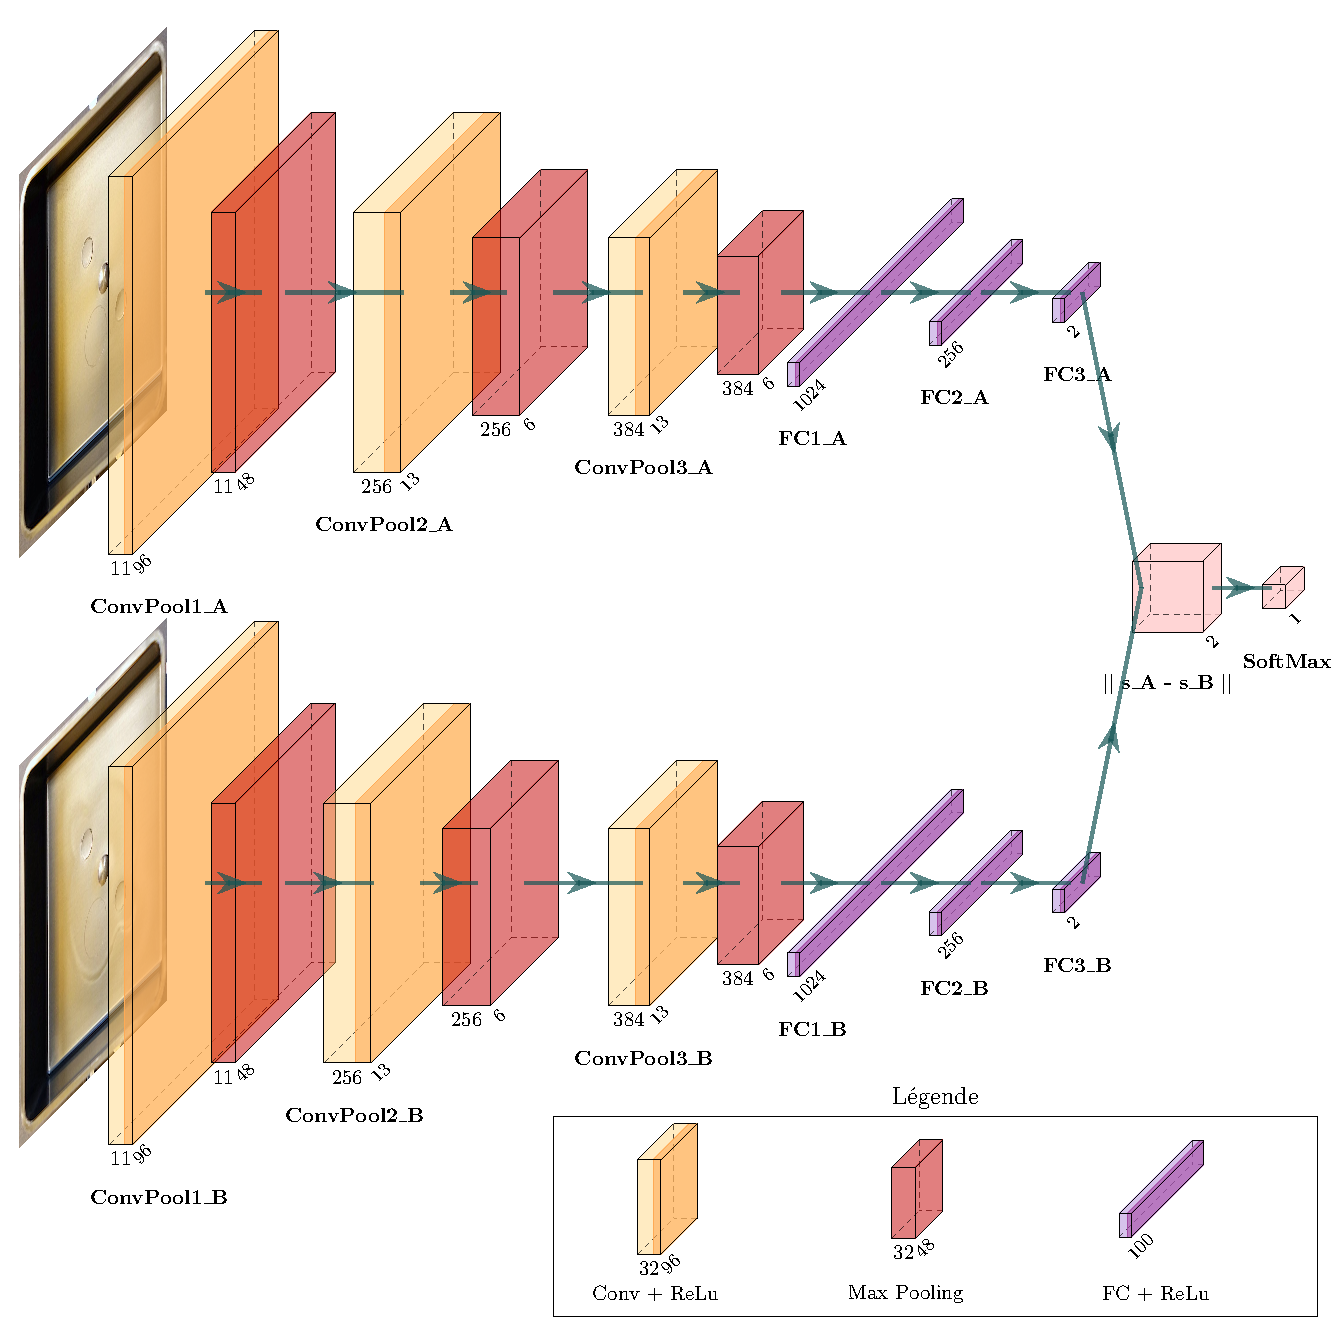
\includegraphics[width=\textwidth,height=\textheight,keepaspectratio]{../Chap4/Figures/siamese.pdf}
    \caption{Architecture d'un réseau siamois.}
    \label{fig:siamese}
\end{figure}

La fonction de coût de contraste, Équation \ref{eq:contrastive_loss}, se compose de $D_{\mathbf{W}}$ qui est une distance entre les vecteurs en sortie des deux branches du réseau.
Dans le cas le plus simple, c'est la norme Euclidienne $\ell_{2}$ entre les vecteurs $\mathbf{s\_A}$ et $\mathbf{s\_B}$.
Dans cette équation, $D_{\mathbf{W}}$ correspond à la distance entre les matrices de poids $\mathbf{W}$.
La matrice de poids $\mathbf{W}$ est l'ensemble des poids de la branche du réseau précédent cette fonction.
Ainsi, cette fonction de coût de contraste permet de réaliser l'apprentissage des poids du réseau afin de rapprocher dans l'espace latent les images similaires, et au contraire d'éloigner les images non similaires. $\mu \in [0 ; 1]$ est un terme qui permet de balancer les effets d'attraction et de répulsion.

\begin{equation} \label{eq:contrastive_loss}
\begin{split}
\mathcal{L}_{contraste}(0, \mathbf{x}_i, \mathbf{x}_j, \mu) = (1-\mu) \frac{1}{2}\left(D_{\mathbf{W}}\right)^{2}+(\mu) \frac{1}{2}\left\{\max \left(0, m-D_{\mathbf{W}}\right)\right\}^{2}
\\
\text{avec} \ D_{\mathbf{W}} = \left\|f(\mathbf{x}_i) - f(\mathbf{x}_j)\right\|^{2}_{2}
\end{split}
\end{equation}

Afin que la fonction de coût réagisse en particulier aux paires d'images non similaires, on introduit une marge $m$, de valeur supérieure à zéro, qui permet aux paires d'images dont la distance est inférieure à cette marge de ne pas être prises en compte dans le résultat du calcul du coût.
La valeur de la marge peut être choisie selon les résultats de précision et de résidus souhaités.
Dans notre cas de contrôle qualité, nous souhaitons par exemple limiter les faux positifs : les pièces mauvaises qui sont classées comme étant bonnes.
Minimiser le coût de contraste revient à positionner toutes les images d'une même classe en un unique point de l'espace.
Cette propriété peut devenir une limite lorsque des images d'une même classe possèdent des caractéristiques d'autres classes.
C'est pourquoi la fonction de coût de triplet a été proposée et nous la détaillons dans la Section suivante \ref{subsubsec:triplet}.

% https://m2dsupsdlclass.github.io/lectures-labs/slides/09_imbalanced_classif_metric_learning/

\subsubsection{Réseau de neurones de triplets profond} \label{subsubsec:triplet}
Basé sur la même idée que le réseau siamois, le réseau de triplets (\textit{Triplet Networks}) utilise trois réseaux de convolutions en parallèles.
Les trois sorties des convolutions sont utilisées par la fonction de coût de triplets (\textit{Triplet Loss}, Équation \ref{eq:triplet_loss}), proposée par \cite{wang_learning_2014} \citeauthor{wang_learning_2014}, appliquée à la détection des images au contenu similaire.

La fonction de coût de triplets est dérivée de la fonction de coût \textit{LMNN} (\textit{Large Margin Nearest Neighbor}), Équations \ref{eq:lmnn_loss}, proposées par \citeauthor{weinberger_distance_2006} \cite{weinberger_distance_2006}. \textit{LMNN} s'appuient sur la distance de \citeauthor{mahalanobis_generalised_1936} \cite{mahalanobis_generalised_1936} (ici notée $\mathbf{L}_{Maha}$) pour la classification par la méthode des K-plus-proches voisins.
Le terme $\varepsilon_{\text{éloignement}}$ pénalise les petites distances entre les points. Il garantit également que les exemples négatifs sont éloignés des exemples de la classe $i$. $\mu \in [0 ; 1]$ permet de balancer les deux termes (en pratique $\mu=0,5$ est satisfaisant).
\begin{equation} \label{eq:lmnn_loss}
\begin{split}
\mathcal{L}_{\mathrm{LMNN}}(0, \mathbf{x}_i, \mathbf{x}_j, y, \mu)=(1-\mu) \varepsilon_{\text{rapprochement}} + \varepsilon_{\text{éloignement}}
\\
\varepsilon_{\text{rapprochement}}(\mathbf{L}_{Maha})=\sum_{j \leadsto i}\left\|\mathbf{L}\left(\vec{\mathbf{x}}_{i}-\vec{x}_{j}\right)\right\|^{2}
\\
\varepsilon_{\text{éloignement}}(\mathbf{L}_{Maha})=\sum_{i, j \leadsto i} \sum_{n}\left(1-y_{n}\right)\max\left(0, 1+\left\|\mathbf{L}_{Maha}\left(\vec{\mathbf{x}}_{i}-\vec{\mathbf{x}}_{j}\right)\right\|^{2}-\left\|\mathbf{L}_{Maha}\left(\vec{\mathbf{x}}_{i}-\vec{\mathbf{x}}_{n}\right)\right\|^{2}\right)
\\
\end{split}
\end{equation}

Cette méthode est proche de la méthode employée par les Machines à Vecteurs Supports (\textit{Support Vector Machines}) : maximiser la marge séparant les classes dans l'espace métrique appris.
La fonction de coût $\varepsilon_{\text{éloignement}}$ est composée du coût de \textit{hinge} (\textit{Hinge loss}, $\mathcal{L}_{Hinge}(z)=\max (0, z)$) aussi utilisé par les \textit{SVM}.
Cependant, contrairement aux \textit{SVM}, la méthode peut être utilisée pour de la classification multi-classes, sans modification et avec de meilleures performances que l'algorithme \textit{SVM}.

Récemment, \citeauthor{schroff_facenet_2015} \cite{schroff_facenet_2015} ont fait évoluer le coût $\mathcal{L}_{\mathrm{LMNN}}$ et propose la fonction de coût de triplet $\mathcal{L}_{\mathrm{triplet}}$ Équation \ref{eq:triplet_loss}.
Trois images sont présentées en entrée au réseau : une image A de référence, une image Positive d'une catégorie et une image Négative d'une autre catégorie.
La distance entre l'image R de Référence et l'image P Positive doit être plus petite que la distance entre l'image R et l'image N Négative.
La fonction de coût de triplets cherche à entrainer le réseau afin séparer la paire positive $($image R, image P$)$ de la paire négative $($image A, image N$)$ par une distance de marge : c'est à dire minimiser la distance entre $($images R, image P$)$ et maximiser la distance entre $($image R, image N$)$.

Les travaux de \citeauthor{wang_learning_2014} \cite{wang_learning_2014} et \citeauthor{schroff_facenet_2015} \cite{schroff_facenet_2015} proposent également l'utilisation d'architectures de réseaux de convolutions profonds issues de la littérature sans les modifier (\textit{AlexNet} modifié \cite{zeiler_visualizing_2013} et \textit{GoogleLeNet-InceptionV1} \cite{szegedy_going_2014}), à la manière de boites noires, et d'entrainer l'ensemble du réseau ainsi constitué.
A la suite du réseau, la norme Euclidienne entre les trois branches est calculée.
Ainsi, la distance entre toutes les images qui sont de la même catégorie sera petite, tandis que la distance entre les paires d'images de différentes catégories sera grande.
\citeauthor{wu_sampling_2017} \cite{wu_sampling_2017} justifient l'utilisation de la norme Euclidienne au lieu de la norme Euclidienne élevée au carré utilisée dans \citeauthor{schroff_facenet_2015} \cite{schroff_facenet_2015}.

A la différence de la fonction de coût de contraste (Équation \ref{eq:contrastive_loss}) qui cherche à positionner toutes les images d'une même classe en un unique point de l'espace latent, la fonction de coût de triplet cherche à maximiser une marge entre chaque paire d'images de catégories différentes.
Ainsi, les images similaires peuvent être positionnées librement à des points différents de l'espace latent, sous réserve que la condition sur la marge entre les catégories différentes soit remplie.

\begin{equation} \label{eq:triplet_loss}
\mathcal{L}_{triplet}\left(\mathbf{x}_r, \mathbf{x}_p, \mathbf{x}_n\right) = \operatorname{max}\left(0,  \left\|f\left(\mathbf{x}_{i}^{R}\right)-f\left(\mathbf{x}_{i}^{P}\right)\right\|_{2}-\left\|f\left(\mathbf{x}_{i}^{R}\right)-f\left(\mathbf{x}_{i}^{N}\right)\right\|_{2} + \alpha\right)
\end{equation}

$\mathbf{x}_{i}^{R}$ représente l'ensemble des images de référence, $\mathbf{x}_{i}^{P}$ l'ensemble des images de catégorie positive et $\mathbf{x}_{i}^{N}$ de catégorie négative.

Le problème majeur de cette fonction de coût est que sur l'ensemble d'un jeu de données, la majorité des triplets d'images répondront à cette contrainte.
Dans ce cas, le réseau ne pourra pas optimiser rapidement ses poids sur cette condition, car la fonction de coût sera le plus souvent constante.
C'est pourquoi il est nécessaire de sélectionner judicieusement des triplets d'images qui sont difficiles à discriminer, en commençant au début par des triplets faciles, puis en raffinant la difficulté au fur et à mesure de l'apprentissage par descente de gradient.

Pour l'entrainement optimale du réseau, il s'agit de sélectionner, pour toutes images $\mathbf{x}_{i}^{R}$ de référence, les images $\mathbf{x}_{i}^{P}$ et $\mathbf{x}_{i}^{N}$ telles que les Équations \ref{eq:triplet_cond1} soient remplies.
\begin{equation} \label{eq:triplet_cond1}
\begin{split}
\mathbf{x}_{i}^{P}=\operatorname{argmax}_{\mathbf{x}_{i}^{P}}\left\|f\left(\mathbf{x}_{i}^{R}\right)-f\left(\mathbf{x}_{i}^{P}\right)\right\|_{2}
\\
\mathbf{x}_{i}^{N}=\operatorname{argmin}_{\mathbf{x}_{i}^{N}}\left\|f\left(\mathbf{x}_{i}^{R}\right)-f\left(\mathbf{x}_{i}^{N}\right)\right\|_{2}
\end{split}
\end{equation}

Les auteurs de \cite{schroff_facenet_2015} appellent ces paires d'images "négatives-difficiles" et "positives-difficiles". 
Ainsi, les images "négatives-difficiles" sont celles qui possèdent le plus de similarités avec l'image de référence, mais qui devront être les plus éloignées de l'image de référence après l'apprentissage.
Réciproquement, les images "positives-difficiles" sont celles qui sont les moins similaires avec l'image de référence, mais qui devront être les plus rapprochées de l'image de référence après l'apprentissage.
La figure \ref{fig:triplet_neg} présente les trois cas d'images Négatives $\mathbf{x}_{i}^{N}$ possibles pour un couple d'images (Référence, Positive) :
\begin{itemize}
    \item Négatives-faciles : $\left\|f\left(\mathbf{x}_{i}^{R}\right)-f\left(\mathbf{x}_{i}^{N}\right)\right\|_{2} \ > \ \left\|f\left(\mathbf{x}_{i}^{R}\right)-f\left(\mathbf{x}_{i}^{P}\right)\right\|_{2}+\alpha$ \ , dans ce cas $\mathcal{L}_{triplet}=0$.
    \item Négatives-modérées : $\left\|f\left(\mathbf{x}_{i}^{R}\right)-f\left(\mathbf{x}_{i}^{P}\right)\right\|_{2} < \left\|f\left(\mathbf{x}_{i}^{R}\right)-f\left(\mathbf{x}_{i}^{N}\right)\right\|_{2} < \left\|f\left(\mathbf{x}_{i}^{R}\right)-f\left(\mathbf{x}_{i}^{N}\right)\right\|_{2}+\alpha$, avec ici $0 < \mathcal{L}_{triplet} < \alpha$.
    \item Négatives-difficiles : $\left\|f\left(\mathbf{x}_{i}^{R}\right)-f\left(\mathbf{x}_{i}^{N}\right)\right\|_{2} \ < \ \left\|f\left(\mathbf{x}_{i}^{R}\right)-f\left(\mathbf{x}_{i}^{P}\right)\right\|_{2}$ \ , on a $\mathcal{L}_{triplet} > \alpha$.
\end{itemize}

\begin{figure}[hbtp]
    \centering
    \begin{tikzpicture}
    \filldraw[fill=green!20!white, draw=black] (0,0) rectangle (10, 7);
    \filldraw[fill=orange!30!white, draw=black] (5,3.4) circle (3.1);
    \filldraw[fill=red!30!white, draw=black] (5,3.4) circle (1.7);
    \draw[Latex-Latex, line width=1] (6.68,3.76)--(8.0,4.1) node[midway,above,sloped] {marge $\alpha$};
    \filldraw[fill=white, draw=blue] (5,3.4) circle (0.25);
    \node[text centered] at (5,3.4) {R};
    \filldraw[fill=white, draw=green] (6.68,3.4) circle (0.25);
    \node[text centered] at (6.68,3.4) {P};
    \node[text centered] at (5.95,5.32) {Nég.-modérées};
    \node[text centered] at (5,3.95) {Nég.-difficiles};
    \node[text centered] at (7.8,6.5) {Négatives-faciles};
    \end{tikzpicture}

    \caption{Trois différents types d'images Négatives possibles pour un couple d'images (Référence, Positive). Figure inspirée de l'\href{https://omoindrot.github.io/triplet-loss}{article de blog de O. Moindrot}.}
    \label{fig:triplet_neg}
\end{figure}

La condition de similarité maximale sur les images négatives peut cependant créer un minima local lors de l'apprentissage, en ne sélectionnant que certaines images du jeu de données, ce qui empêche  la convergence.
Il est nécessaire d'introduire une certaine variabilité dans les images négatives.
C'est pourquoi \cite{schroff_facenet_2015} introduit une troisième condition, Équation \ref{eq:triplet_cond2}.

\begin{equation} \label{eq:triplet_cond2}
\left\|f\left(\mathbf{x}_{i}^{R}\right)-f\left(\mathbf{x}_{i}^{P}\right)\right\|_{2} \ < \ \left\|f\left(\mathbf{x}_{i}^{R}\right)-f\left(\mathbf{x}_{i}^{N}\right)\right\|_{2}
\end{equation}

Il s'agit de sélectionner des images "négatives-modérées", c'est à dire des images qui sont plus éloignées de l'image de référence que les images positives, mais qui ont une similarité élevée avec l'image de référence.
Dans la même démarche, \citeauthor{shi_embedding_2016} \cite{shi_embedding_2016} proposent de sélectionner en plus les images "positives-modérées".
La Figure \ref{fig:triplet_learning} récapitule la méthode d'apprentissage d'un réseau de triplets.
\begin{figure}[hbtp]
    \centering
    \begin{tikzpicture}[remember picture]
    \filldraw[fill=green!20!white, draw=black] (0,0) rectangle (7, 7);
    \filldraw[fill=orange!30!white, draw=black] (3.5,3.4) circle (3.1);
    \filldraw[fill=red!30!white, draw=black] (3.5,3.4) circle (1.7);
    \draw[Latex-Latex, line width=1] (5.18,3.76)--(6.5,4.1) node[midway,above,sloped] {marge $\alpha$};
    \filldraw[fill=white, draw=blue] (3.5,3.4) circle (0.25);
    \node[text centered] at (3.5,3.4) {R};
    \filldraw[fill=white, draw=green] (5.18,3.4) circle (0.25);
    \node[text centered] at (5.18,3.4) {P};
    \draw[-Latex, line width=1] (3.75,3.4)--(4.92,3.4);
    \filldraw[fill=white, draw=red] (5.1,5.1) circle (0.25);
    \node[text centered] at (5.1,5.1) {N};
    \draw[-Latex, line width=1] (3.66,3.60)--(4.92,4.92);
    
    \path ([xshift=-2cm]current bounding box.north east) -- 
    ([yshift=4.2cm]current bounding box.south east) coordinate[midway] (2BL);
    \end{tikzpicture}
    \hspace{0.795cm}
    \begin{tikzpicture}[remember picture]
    \filldraw[fill=green!20!white, draw=black] (0,0) rectangle (7, 7);
    \filldraw[fill=orange!30!white, draw=black] (3.5,3.4) circle (3.1);
    \filldraw[fill=red!30!white, draw=black] (3.5,3.4) circle (1.7);
    \draw[Latex-Latex, line width=1] (5.18,3.76)--(6.5,4.1) node[midway,above,sloped] {marge $\alpha$};
    \filldraw[fill=white, draw=blue] (3.5,3.4) circle (0.25);
    \node[text centered] at (3.5,3.4) {R};
    \filldraw[fill=white, draw=green] (5.18,3.4) circle (0.25);
    \node[text centered] at (5.18,3.4) {P};
    \draw[-Latex, line width=1] (3.75,3.4)--(4.92,3.4);
    \filldraw[fill=white, draw=red] (6.2,6.2) circle (0.25);
    \node[text centered] at (6.2,6.2) {N};
    \draw[-Latex, line width=1] (3.66,3.60)--(6.02,6.02);
    
    \path ([xshift=2cm]current bounding box.north west) -- 
    ([yshift=4.2cm]current bounding box.south west) coordinate[midway] (2BR);
    \end{tikzpicture}
    
    \tikz[overlay,remember picture]{\draw[-Latex,ultra thick,bend left] (2BL) to node[above,sloped]{Apprentissage} (2BL-|2BR);}
    
    \caption{Principe de l'apprentissage d'un réseau de triplets. Figure inspirée de \cite{schroff_facenet_2015}.}
    \label{fig:triplet_learning}
\end{figure}

Le calcul des Équations \ref{eq:triplet_cond1} pour la sélection d'images sur l'ensemble du jeu de données est très coûteux.
C'est pourquoi ce calcul est traditionnellement réalisé en amont de l'apprentissage. De plus, pour sélectionner les images parmi l'ensemble du jeu de données, il est nécessaire que le jeu de données puisse être chargé dans la mémoire de travail de la machine qui effectue le calcul des conditions.
Les jeux de données actuels sont souvent trop volumineux pour pouvoir être chargés en entier dans la mémoire.
C'est pourquoi il a été proposé de réaliser ce calcul pendant l'apprentissage \cite{wang_learning_2014,schroff_facenet_2015}.
Pour maximiser les performances du calcul de la méthode d'optimisation des poids par descente de gradient sur processeur graphique, les données d'apprentissage sont séparées en paquets (\textit{mini-batch}) avant d'être présentées en entrée du réseau pour l'apprentissage.
Pour chaque paquet, les couples d'images "négatives-modérées" sont alors sélectionnées de manière itérative, en parallèle de l'apprentissage.
Récemment, \citeauthor{hermans_defense_2017} \cite{hermans_defense_2017, yu_correcting_2018} proposent de sélectionner les images négatives-difficiles dans les paquets.
Sur leur problème spécifique de la détection de visages, ils montrent qu'il n'est pas nécessaire d'introduire la condition de marge modérée car le fait de découper le jeu de données en paquets aléatoires garantie une certaine variété d'images dans les paquets.

\begin{figure}[hbtp]
    \centering
    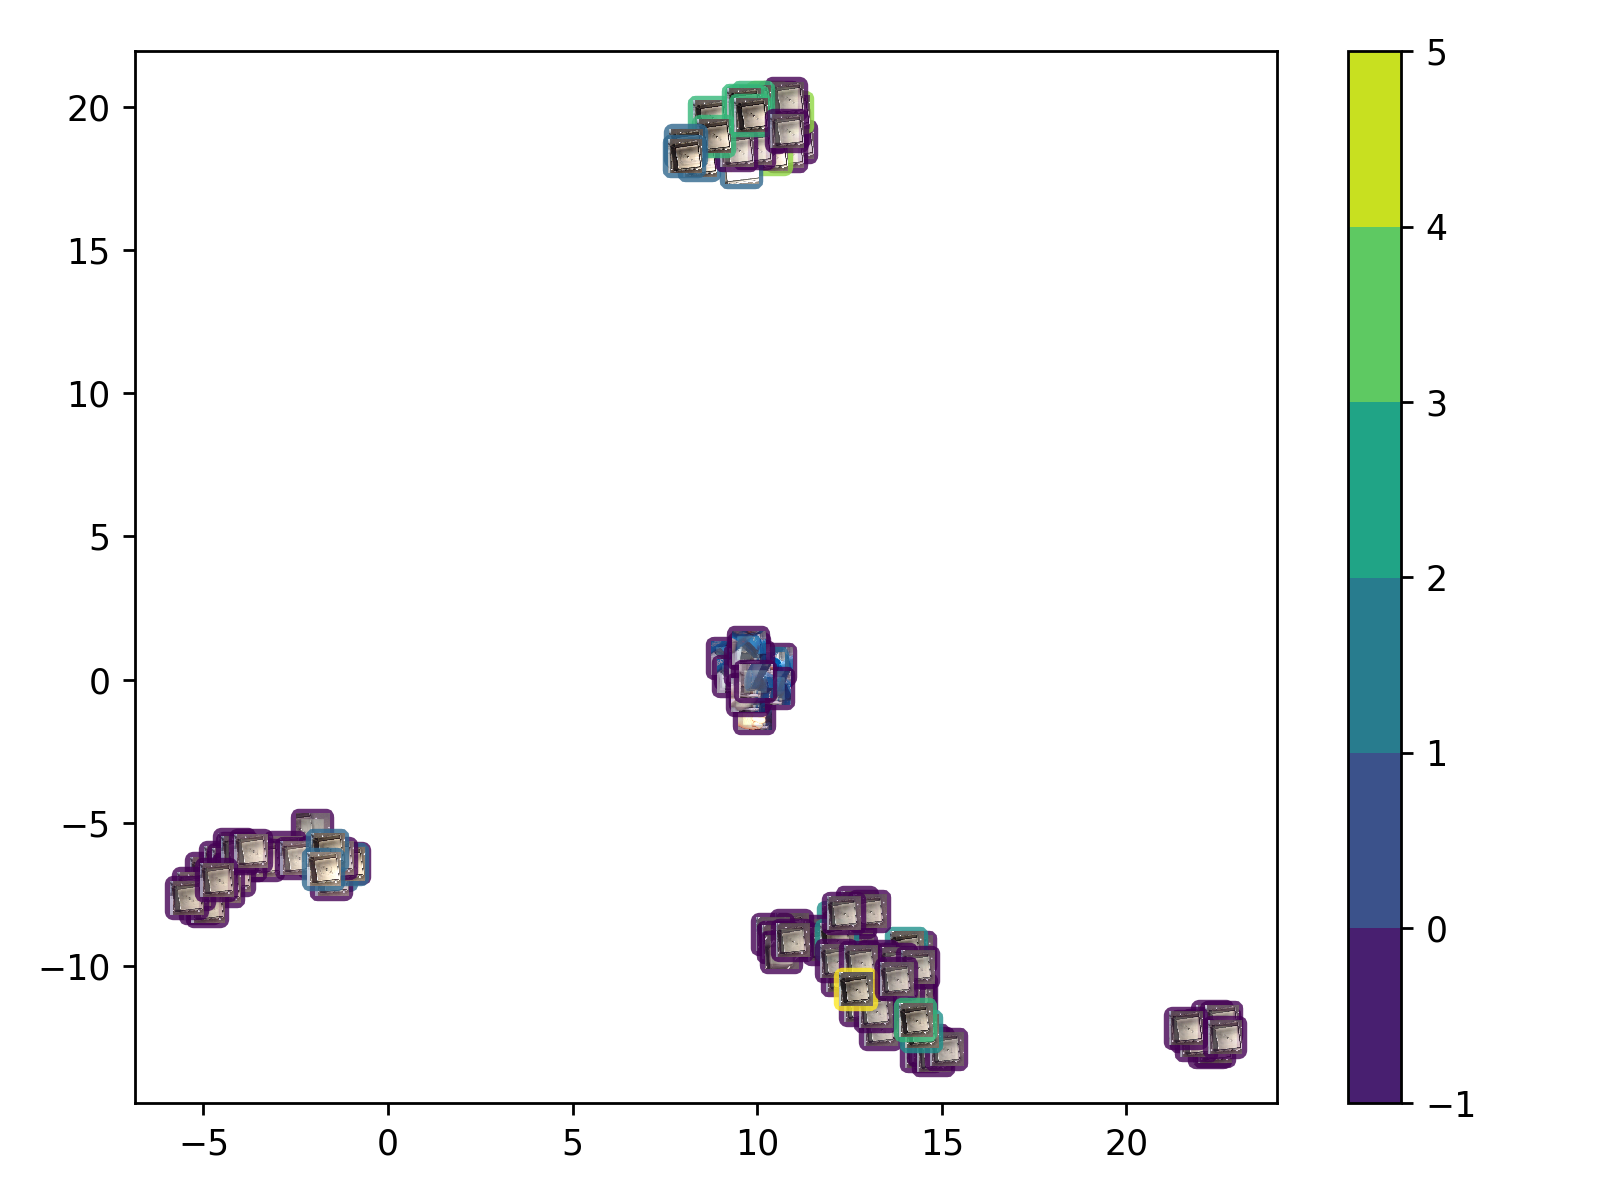
\includegraphics[width=0.95\textwidth,height=\textheight,keepaspectratio]{../Chap4/Figures/visualize_UMAP_pixel_space_10_0_5corr.png}
    \caption{Projection par \textit{t-SNE} à partir des valeurs de la dernière couche d'un réseau de triplet. L'échelle 1-5 correspond aux niveaux de qualité évalués par les experts humains ; -1 correspond aux pièces non annotées.}
    \label{fig:triplet_result}
\end{figure}

La Figure \ref{fig:triplet_result} présente les valeurs de la dernière couche d'un réseau de triplets, de 200, projetée en deux dimensions par l'algorithme \textit{t-SNE} §\ref{subsubsec:tsne}.
Les différentes classes annotées par les experts humains sont bien séparées.
Les pièces non annotées sont également positionnées dans les bonnes classes.
Enfin, il est intéressant d'observer qu'un paquet correspondant à une erreur de mesure, comme par exemple l'absence de pièces et la capture du bras robotique préhenseur est mis en évidence.

L'apprentissage de métrique est un domaine de recherche actif.
\citeauthor{sohn_improved_2016} \cite{sohn_improved_2016} généralisent par exemple ces méthodes à N-paires d'images et montre l'intérêt d'une fonction de coût à 72-paires en comparaison des triplets (3-paires).
\citeauthor{song_deep_2015} \cite{song_deep_2015} proposent une méthode d'adaptation de domaine : un modèle pré-appris peut être compléter à l'aide de nouveaux échantillons.
\cite{wang_deep_2017} \citeauthor{wang_deep_2017} proposent d'utiliser une fonction de coût basée sur une projection dans un espace angulaire.
\citeauthor{duan_deep_2018} \cite{duan_deep_2018} proposent la méthode \textit{DAML} (\textit{Deep Adversarial Metric Learning}) qui utilise un réseau antagoniste génératif (détaillé dans la Section \ref{subsubsec:GAN}) afin de produire une image négative-difficile artificielle, à partir d'un triplet d'images défini.
Les résultats obtenus montrent l'intérêt de la méthode dans le cas où le nombre d'échantillons est faible.
Dernièrement, \citeauthor{zheng_hardness-aware_2019} \cite{zheng_hardness-aware_2019} proposent une comparaison de ces méthodes (N-paires, métrique angulaire et \textit{DAML}) sur trois jeux de données de références.

% Local similarity-aware deep feature embedding propose le Position-Dependent Deep Metric (PDDM)

% CVPR2019 Variational Prototyping-Encoder: One-Shot Learning with Prototypical Images https://github.com/mibastro/VPE

% [5] Yi Sun, Xiaogang Wang, Xiaoou Tang, Deep Learning Face Representation by Joint Identification-Verification, NIPS 2014

% Information Theory Malhanobis (ITML) : Kulis, B., Jain, P., Grauman, K.: Fast similarity search for learned metrics. IEEE PAMI 39(12), 2143–2157 (2009)
% https://gombru.github.io/2019/04/03/ranking_loss/
% https://hanxiao.github.io/2017/11/08/Optimizing-Contrastive-Rank-Triplet-Loss-in-Tensorflow-for-Neural/

% Bier - boosting independent embeddings robustly - nice!
% Hard-aware deeply cascaded embedding - caffe
% Deep Metric Learning with Hierarchical Triplet Loss

\subsubsection{Intérêt des méthodes issues de l'apprentissage par renforcement}
Les récents succès des méthodes d'apprentissage par renforcement peuvent également être inclus dans cette section.
À chaque itération, l'algorithme choisit de réaliser une action et il obtient, pour cette action, une récompense, positive en cas d'amélioration de l'objectif, ou négative dans le cas inverse.
L'apprentissage par renforcement est particulièrement adapté au réglage optimal des procédés.
Il est nécessaire de disposer d'un environnement capable de recevoir une action et produire une récompense.
Cet environnement peut être une simulation réaliste de l'environnement, ou bien l'environnement réel.
Dans notre cas, les actions seraient la modification des réglages du procédé et la récompense, la pièce produite.
Cependant, nous ne disposons actuellement pas de simulation informatique réaliste de notre problème. De plus, l'évaluation en conditions réelles nécessite de disposer d'une machine pilotée par l'algorithme, qui produit un minimum de mille pièces.
Néanmoins, dans le contexte d'une production en quantité industrielle, l'utilisation de l'apprentissage par renforcement devient possible. C'est une piste de recherche qui devra être évaluée à la suite de ces travaux.

% \subsubsection{Méthode de méta-apprentissage MAML : Model-Agnostic Meta-Learning}
% TODO: MAML
% Spécifique au one-shot learning.

% https://bair.berkeley.edu/blog/2017/07/18/learning-to-learn/
% Model-Agnostic Meta-Learning for Fast Adaptation of Deep Networks.
% C. Finn, P. Abbeel, S. Levine. In ICML, 2017. (pdf, code)

% How to train your MAML

% https://lilianweng.github.io/lil-log/2018/11/30/meta-learning.html


\subsection{Apprentissage non-supervisé} \label{subsec:unsupervised}
Contrairement aux méthodes précédemment présentées, nous cherchons ici à classer sans aucune assistance d'un expert humain.
Supprimer le besoin d'annotation d'un expert amène deux bénéfices : une disponibilité totale du système et une suppression des risques d'erreurs humaines.
Ces méthodes permettent de réduire la dimension des données et de classifier en utilisant uniquement les hypothèses sur la structure des données, précitées dans la Section \ref{it:manifold_hypothesis}, sans annotation.
La réduction de dimensions est un enjeu important dans notre problématique industrielle.
En effet, les données enregistrées par les capteurs ont un ordre de grandeur de l'ordre du million de valeurs scalaires par pièces.
Le traitement de la mesure doit être effectué sur un système embarqué, intégrable à la ligne de production, qui a une puissance de calcul faible.
Plus la dimension de l'information issue des capteurs est réduite, plus l'inférence de la conformité sera rapide.
De plus, la réduction de l'information est un objectif crucial afin de pouvoir piloter en boucle fermée le procédé.
En effet, le pilotage multivarié des procédés industriels est possible dans un espace de dimensions faibles (de dimensions dix à cent).
Il existe deux grandes classes de méthodes de réduction de dimensions.
Celles-ci s'appuient sur deux démarches distinctes : la factorisation de matrices (ACP §\ref{subsubsec:ACP}, ACP à noyau §\ref{subsubsec:kpca}, Auto-encodeurs) et les graphes de voisinages (K-moyennes §\ref{subsubsec:kmeans}, §\ref{subsubsec:tsne}, §\ref{subsubsec:hdbscan}, §\ref{subsubsec:umap}).
Nous évaluons dans cette section les algorithmes les plus importants que nous utilisons pour répondre à notre problème de contrôle automatique de la conformité des produits.
La réduction de dimensions et le \textit{clustering}\footnote{Nous employons le terme anglais \textit{clustering} en lieu et place du mot français "regroupement", afin de préciser qu'il s'agit de réaliser un regroupement algorithmique des données en paquets de données similaires, et non pas d'autres formes de regroupement.} spectral (aussi appelé "apprentissage de variétés") sont souvent combinées.
Dans un premier temps on réduit la dimension de l'information, puis on regroupe par paquet les échantillons (\textit{clustering}) à partir de l'espace réduit.

\subsubsection{K-moyennes} \label{subsubsec:kmeans}
L'algorithme des K-moyennes (\textit{K-means}), proposé par \citeauthor{macqueen_methods_1967} \cite{macqueen_methods_1967, lloyd_least_1982} cherche à séparer les échantillons $X$ en $C$ groupes de classes telle que la variance soit égale entre les groupes.
C'est une méthode de \textit{clustering} spatial dans l'espace des données initiales.
Soit $c_j$ le barycentre d'un groupe dans l'espace des données, l'algorithme cherche à minimiser la distance Euclidienne des échantillons au point $c$.
Il s'agit de minimiser l'inertie\footnote{L'inertie est la somme des distances Euclidiennes entre les échantillons du groupe.} du groupe d'échantillon $c_j \in C$.
L'algorithme est itératif.
Le nombre de groupes doit être préalablement connu.
La position initiale des points $c_j$ est initialisée aléatoirement.
À chaque itération, les échantillons $\mathbf{x}_i \in X$ sont associés au point $c_j$ le plus proche.
La position de $c_j$ est alors mise à jour comme barycentre des points $\mathbf{x}_i$ qui lui sont associés, Équation \ref{eq:kmeans}.

\begin{equation} \label{eq:kmeans}
C(X) = \arg \ \min _{c_{j} \in C} \ \sum_{j=1}^{n_C} \sum_{i=1}^{n} \left(\left\|\mathbf{x}_{i}-c_{j}\right\|^{2}\right)
\end{equation}

La convergence est nécessairement atteinte mais elle peut être un minimum locale.
Le résultat final est fortement dépendant de la position initiale des points centroïdes $c$.
C'est pourquoi l'algorithme complet est répété de nombreuses fois avec des initialisations de $c_j$ différentes.
La méthode d'initialisation \textit{k-means++}, plus performante, a été proposée par \citeauthor{arthur_kmeans_2007} \cite{arthur_kmeans_2007}. Elle propose de positionner les points centroïdes $c$ de manière à les éloigner au maximum entre eux. Les résultats obtenus sont ainsi meilleurs.
Enfin, la distance Euclidienne $\ell_{2}$ est une métrique qui répond mal aux problèmes en très grandes dimensions ou aux formes de groupes allongées ou irrégulières.
Cette distance ne prend pas en compte la variation de la densité des points dans l'espace.
C'est pourquoi une transformation de l'espace des données est souvent réalisée en amont de cet algorithme (ACP, \textit{kernel trick} ...).
Des méthodes de \textit{clustering} spectral ont alors été proposées pour répondre à cette limite.

La complexité de l'algorithme K-moyennes est de l'ordre de  $\bigO(N \log(N))$.
C'est la méthode de \textit{clustering} la plus efficiente qui existe.

\subsubsection{HDBSCAN} \label{subsubsec:hdbscan}
\citeauthor{ester_densitybased_1996} \cite{ester_densitybased_1996} proposent la méthode \textit{DBSCAN} (\textit{Density-Based Spatial Clustering of Applications with Noise}) qui s'appuie sur l'organisation spatiale, en matière de densité, des données.
L'algorithme distingue en amont trois catégories d'échantillons dans les données.
Pour chaque point $c$, on distingue : les points centraux s'ils sont entourés d'un nombre minimal $MinPts$ de voisins et sont situés dans un rayon $\epsilon$ du point $c$ ; les points de bordures s'ils ont moins de $nb\_min\_points$ voisins et sont situés dans un rayon $\epsilon$ ; et les points de bruit, dont la distance avec $c$ est supérieure à $\epsilon$.
Ainsi, le nombre de paquets est défini par $nb\_min\_points$ et les points de bordures sont associés au paquet par leur point $c$ correspondant.
À la différence de l'algorithme K-moyennes §\ref{subsubsec:kmeans}, l'algorithme \textit{DBSCAN} ne cherche pas à produire des paquets circulaires et les points trop éloignés sont ignorés ce qui le rend robuste aux perturbations.
Néanmoins, les performances de la méthode \textit{DBSCAN} sont limités sur les problèmes où les échantillons ont de grandes dimensions. On cherchera à réduire la dimension de l'information, par exemple lorsque l'on traite des images, avant d'appliquer cette méthode.
Les hyper-paramètres $nb\_min\_points$ et $\epsilon$ doivent être optimisés. Trouver un couple optimal peut être difficile, dans le cas où les données sont réparties de manière fortement non homogène ; c'est à dire lorsque les différences de densités de la répartition des points sont grandes.

Récemment, \citeauthor{campello_densitybased_2013} \cite{campello_densitybased_2013} introduisent la méthode \textit{HDBSCAN} (\textit{Density-Based Clustering Based on Hierarchical Density Estimates}) qui fait évoluer \textit{DBSCAN} en prenant en compte l'organisation spatiale des données.
\textit{HDBSCAN} ne nécessite pas de paramètre $\epsilon$.

De nombreuses méthodes de \textit{clustering} s'appuient sur l'organisation hiérarchique des données.
C'est le \textit{clustering} hiérarchique, qui utilise les arbres binaires de tri.
Le résultat est souvent visualisé sous forme de dendrogrammes.
Une évolution du \textit{clustering} hiérarchique ajoute l'utilisation de l'analyse spectrale.
Ce sont les méthodes de \textit{clustering} spectral qui proposent des solutions à ces limites.
Il s'agit d'utiliser les relations entre les échantillons au sein des paquets, par la construction de graphes et par l'analyse spectrale, c'est à dire l'utilisation des vecteurs propres des données.
Nous invitons le lecteur à consulter l'excellent tutoriel \citetitle{vonluxburg_tutorial_2007} \cite{vonluxburg_tutorial_2007} sur les méthodes de \textit{clustering} spectrales, qui ne peuvent être approfondies dans le cadre de ce travail.

\begin{figure}[hbtp]
    \centering
    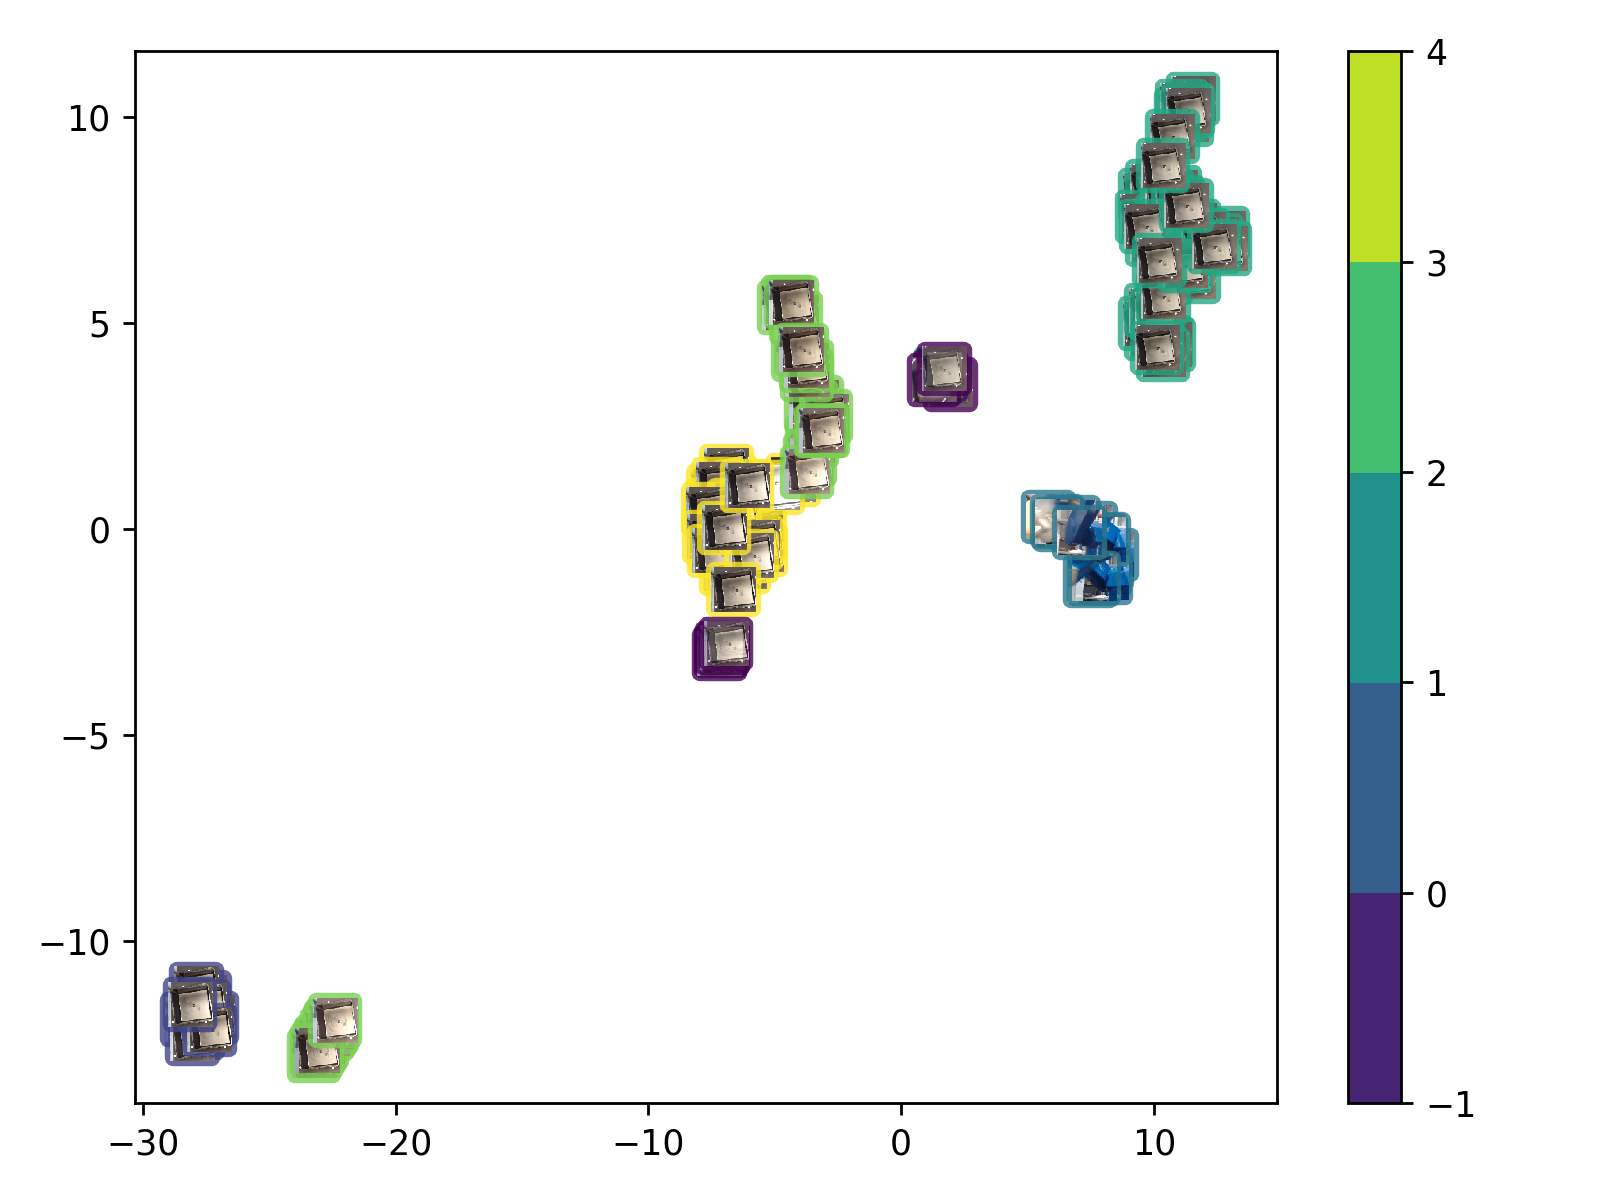
\includegraphics[width=0.95\textwidth,height=\textheight,keepaspectratio]{../Chap4/Figures/visualize_HDBSCAN_clusters_pixel_space.png}
    \caption{Projection par \textit{UMAP} à partir de la valeur des pixels des images. L'échelle -1 à 4 correspond aux clusters obtenus par \textit{HDBSCAN}.}
    \label{fig:hdbscan}
\end{figure}
% rand score 0.320, mutual info score 0.410

La Figure \ref{fig:hdbscan} présente les clusters obtenus par l'algorithme \textit{HDBSCAN}.
La dimension des données a préalablement été réduite par l'algorithme \textit{UMAP} §\ref{subsubsec:umap}.
Les différents niveaux de qualité annotés par l'expertise humaine sont détectés.

\subsubsection{Analyse en Composante Principale} \label{subsubsec:ACP}
Dès 1901, \citeauthor{pearson_lines_1901, hotelling_analysis_1933} \cite{pearson_lines_1901, hotelling_analysis_1933} proposent la méthode d'Analyse en Composante Principale (\textit{Principal Component Analysis}).
C'est la méthode de réduction de dimensions de référence qui s'appuie sur une factorisation de la matrice représentative des données.
Pour un jeu de données $X$ de $N$ échantillons, on calcule la matrice de covariance $\overline{C}$, Équation \ref{eq:cov}.

\begin{equation} \label{eq:cov}
\overline{C} = \operatorname{cov}(X)=\frac{1}{N} \sum_{n=1}^{N}(x_n-\overline{x}) \cdot (x_n-\overline{x})^{\mkern-1.5mu\mathsf{T}}
\end{equation}
% (DIN) EN ISO 80000-2:2013 Transpose: " X^{\mkern-1.5mu\mathsf{T}} " https://tex.stackexchange.com/a/217623

\begin{equation} \label{eq:pca}
\lambda\left(X \cdot \mathbf{V}\right)=\left(X \cdot \overline{C} \cdot \mathbf{V}\right)
\end{equation}

Soit $m$ le nombre de variables par échantillons. Les vecteurs propres $\mathbf{v}_k$ (avec $1 \leq k \leq N$, de la matrice de covariance $\overline{C}$ sont appelés les composantes principales de $X$, Équation \ref{eq:pca}.
Les valeurs propres $\lambda_k$ sont utilisées pour ordonner les vecteurs propres $\mathbf{v}_k$, dans l'ordre croissant de la variance des données exprimées par chaque vecteur propre.
On obtient un espace de dimensions réduites où l'on peut projeter les données.
La réalisation d'une ACP entraine nécessairement une réduction de la variance, en comparaison de la variance de l'ensemble des échantillons du jeu de données initial.
La valeur de cette réduction indique la perte d'informations liée à l'ACP.
Dans ce travail, nous serons satisfaits des ACP qui ne font perdre que 1\% de la variance des données initiales.
On choisira le nombre $k$ de vecteurs supports en fonction de ce critère.
Dans notre application, cinquante vecteurs supports sont suffisants. 

L'Analyse en Composante Principale peut être employée comme méthode de réduction de l'information, par transformation linéaire.
Nous pouvons appliquer une ACP à $k$ composantes sur l'image brute, ce qui compresse l'information dans un vecteur de dimension $k$.
Puis nous appliquons la transformée inverse pour obtenir une reconstruction.
La Figure \ref{fig:pca_reconstruction} montre la capacité de l'ACP à encoder les caractéristiques d'une image, en fonction du nombre de composantes.
Des artefacts de couleurs (ici vertes) sont présents.
L'erreur de reconstruction est la différence des valeurs des pixels entre l'image originale et l'image reconstruite.
Le graphique \ref{fig:pca_plot} montre l'évolution de la qualité de reconstruction en fonction de la proportion de la variance conservée.
On observe que l'erreur diminue lorsque le nombre de composantes et la variance conservée augmente.
Il est intéressant d'observer que pour 5 composantes, ce sont les détails des côtés de la pièce et des défauts du fond de la pièce qui ne sont pas représentés.
Nous nous intéressons; dans le cadre de notre problématique de contrôle de la conformité, à ces défauts, mais l'ACP prend en compte en priorité les caractéristiques globales de l'image.
Lorsque l'on utilise 100 composantes, l'erreur de reconstruction est négligeable.
Des artefacts restent néanmoins présents.
Dans les sections suivantes, nous étudierons des méthodes qui permettent de supprimer la présence d'artefacts et de prendre en compte les caractéristiques locales des images.

\begin{figure}[htbp]
    \centering
    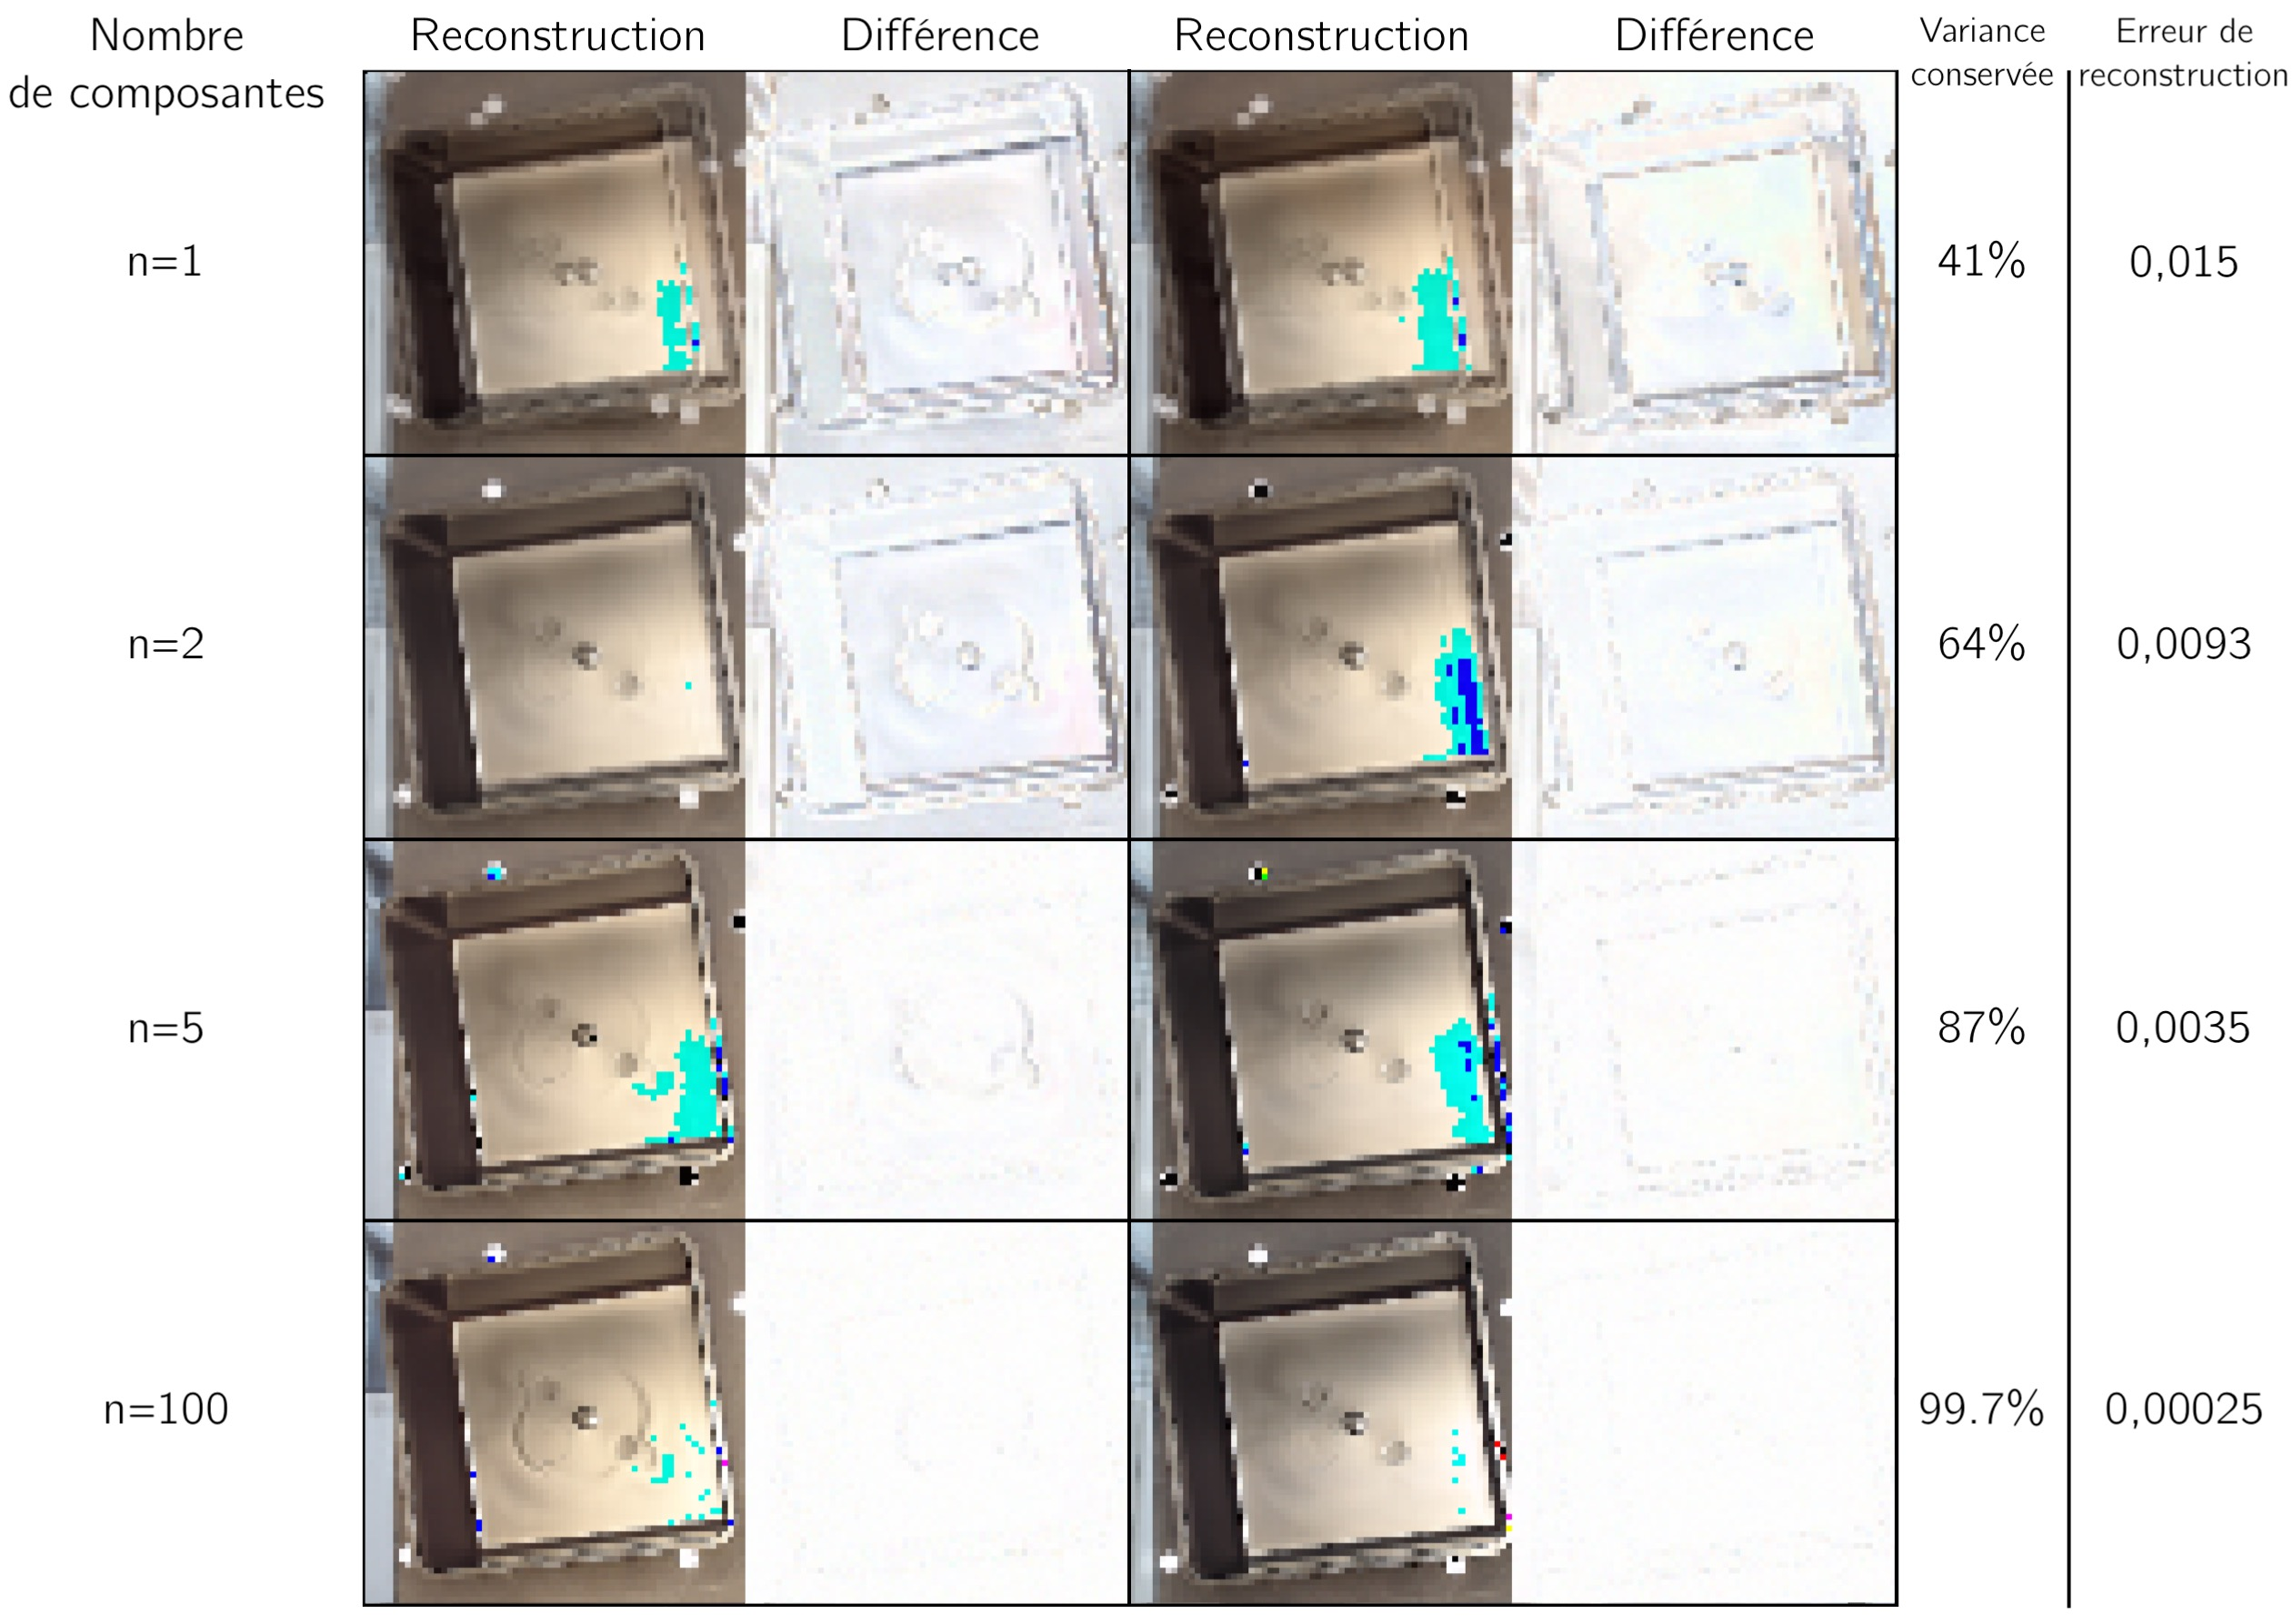
\includegraphics[width=1\textwidth,height=\textheight,keepaspectratio]{../Chap4/Figures/visualize_reconstructed_PCA_components_images.jpg}
    \caption{Compression par ACP.}
    \label{fig:pca_reconstruction}
\end{figure}

\begin{figure}[hbtp]
    \centering
    \begin{adjustbox}{width=0.80\textwidth}
        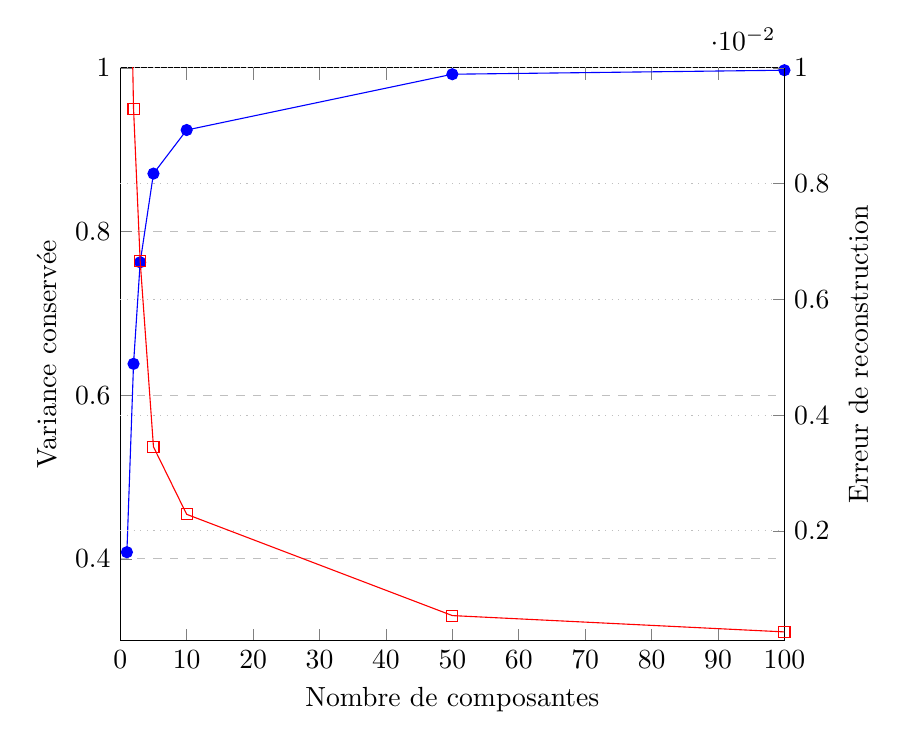
\begin{tikzpicture}
        % let both axes use the same layers
        \pgfplotsset{
            % set layers,
            xlabel=x-axis,
            legend columns=-1,
            legend style={draw=none},
            legend to name=named,
        }
        \begin{axis}[
        set layers,axis background,
        scale only axis,
        xmin=0, xmax=100,
        axis y line*=left,
        legend style={at={(0.5,-0.2)},anchor=north},
        xlabel={Nombre de composantes},
        ylabel style = {align=center},
        ylabel={Variance conservée}, % \ref{pgfplots:plot1}
        xtick={0,10,20,30,40,50,60,70,80,90,100},
        ymin=0.3, ymax=1.0,
        ytick={0.4,0.6,0.8,1.0},
        ymajorgrids=true,
        grid style=dashed,%gray
        ]
        \addplot [color=blue,mark=*]
        table{
            1 0.408233
            2 0.638416
            3 0.762465
            5 0.870857
            10 0.924131
            50 0.992305
            100 0.997201
        };
        % \addlegendentry{Erreur de reconstruction}, HINT: should be added on next axis with \addlegendimage
        \label{plot:pca_var}
        \end{axis}
        \begin{axis}[
        scale only axis,
        xmin=0, xmax=100,
        axis y line*=right,
        axis x line=none,
        ylabel style={align=center},
        ylabel={Erreur de reconstruction}, % \ref{pgfplots:plot2}
        % y dir=reverse,
        % ymode=log,
        ymin=0.0001, ymax=0.01,
        % ytick={0.0001, 0.001,0.01},
        ymajorgrids=true,
        % grid style=dashed,
        major grid style=dotted,
        axis background,
        ]
        \addlegendimage{/pgfplots/refstyle=plot:pca_var}\addlegendentry{Variance conservée}
        \addplot [color=red,mark=square]
        table{
            1 0.015433
            2 0.009297
            3 0.006661
            5 0.003452
            10 0.002285
            50 0.000535
            100 0.000253
        };
        \addlegendentry{Erreur de reconstruction},
        \label{plot:pca_mse}
        \end{axis}
        %
        \end{tikzpicture}
    \end{adjustbox}
    \\
    \ref{named}
    \caption{Qualité de la compression par \textit{ACP} en fonction du nombre de composantes.}
    \label{fig:pca_plot}
\end{figure}

\begin{figure}[hbtp]
    \centering
    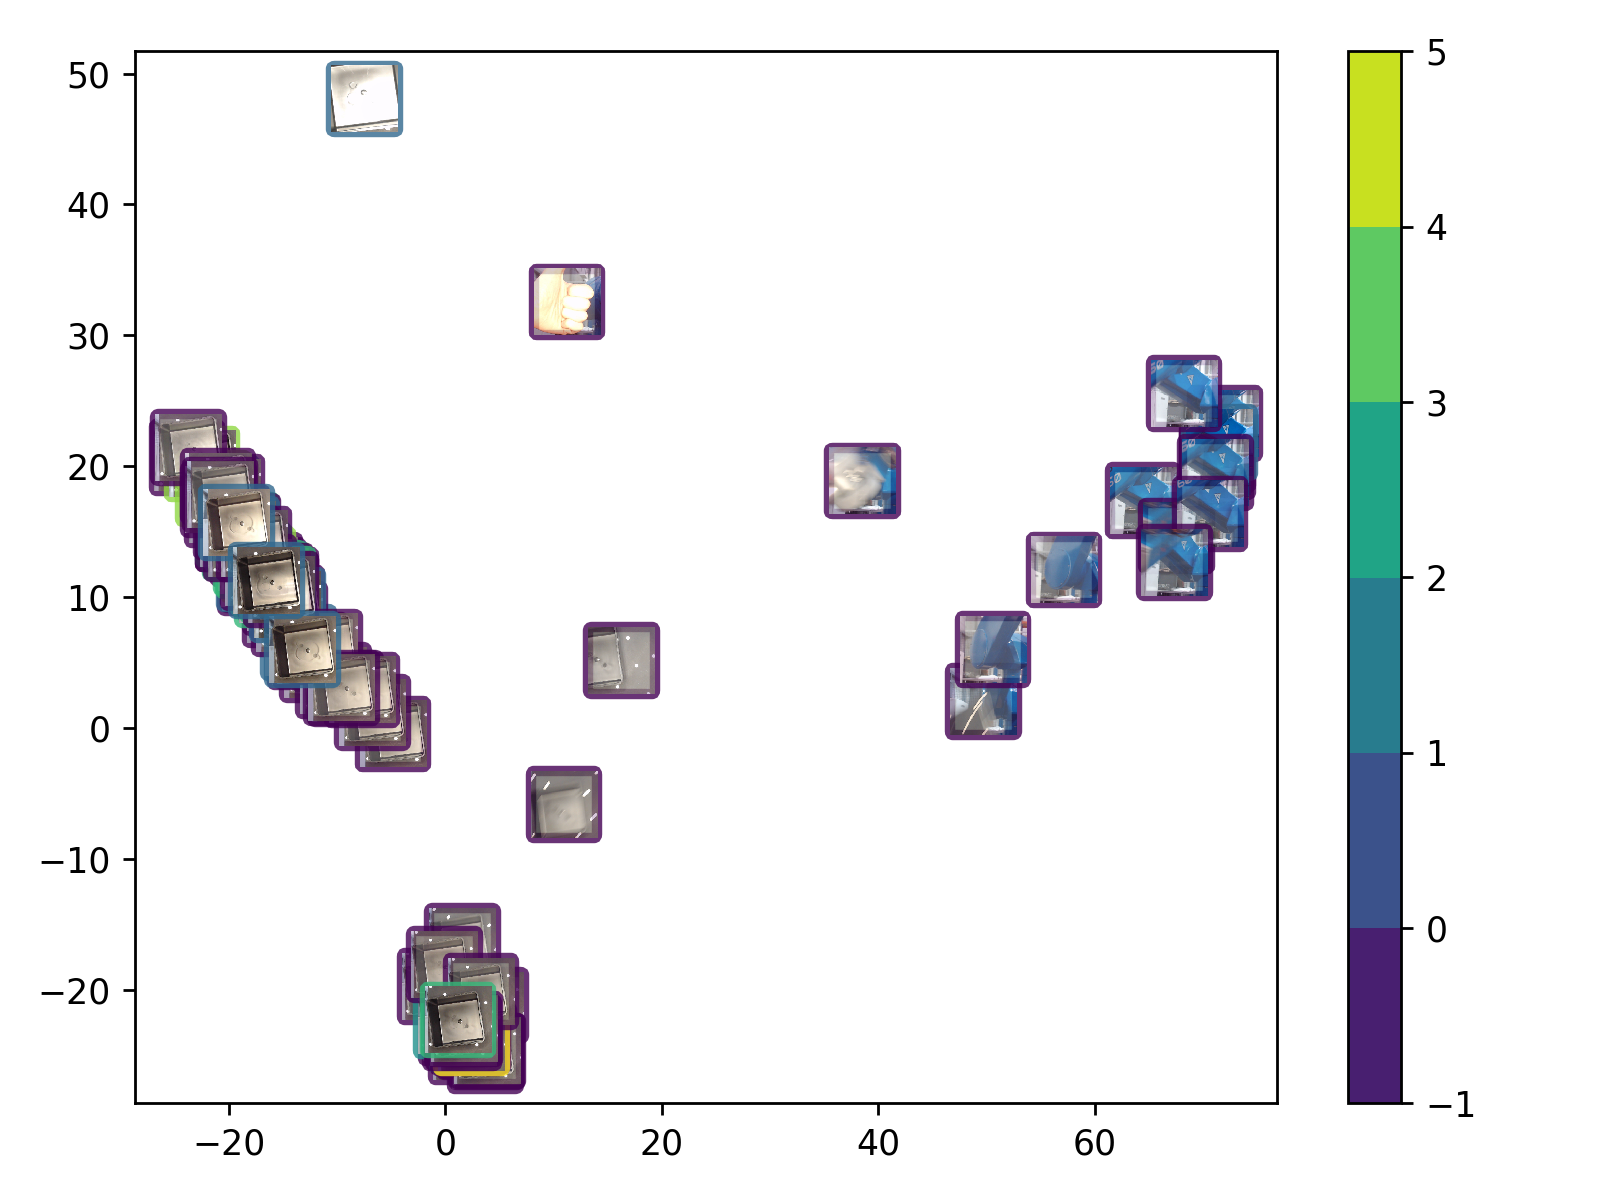
\includegraphics[width=0.95\textwidth,height=\textheight,keepaspectratio]{../Chap4/Figures/visualize_PCA_pixel_space.png}
    \caption{Projection par \textit{ACP} à partir de la valeur des pixels des images. L'échelle 1-5 correspond aux niveaux de qualité évalués par les experts humains ; -1 correspond aux pièces non annotées.}
    \label{fig:ACP}
\end{figure}

La Figure \ref{fig:ACP} présente les valeurs des deux dimensions obtenues pour chaque pièce en appliquant une ACP sur la valeur des pixels bruts de l'image.
On observe une séparation intéressante des images qui ne contiennent pas de pièce, mais par exemple le bras robotique préhenseur.
En revanche, seuls deux paquets sont mis en évidences, parmi lesquels des pièces de bonnes qualité et des pièces de mauvaises qualité sont mélangées.
L'ACP réalisée sur les pixels bruts est limitée aux motifs globaux de l'image.
Il est nécessaire de réaliser un prétraitement des images pour extraire les motifs pertinents sur notre problème avant d'appliquer une ACP.
L'expertise humaine est requise pour choisir les méthodes judicieuses de prétraitement à appliquer.
Nous détaillons des approches de ce type dans la Section \ref{sec:extraction}.
L'ACP utilise ici deux uniques composantes.
Comme présenté dans les figures \ref{fig:pca_reconstruction} et \ref{fig:pca_plot}, une centaine de composantes permettent de modéliser la variance de notre jeu de données de manière satisfaisante.
Avec deux composantes, la perte de variance est de 36 \%, ce qui est important.
Il sera judicieux d'utiliser un nombre de composantes plus important, ou bien d'utiliser une méthode plus robuste tels que le \textit{t-SNE} \ref{subsubsec:tsne} ou \textit{UMAP} \ref{subsubsec:umap}.

Le calcul de la matrice de covariance $\overline{C}$ a une complexité de l'ordre de $\bigO(m^{2} \cdot N)$.
La décomposition en valeur propre a une complexité $\bigO(m^{3})$.
La complexité de l'ACP est $\bigO(m^{2} \cdot N+m^{3})$.
Soit, pour un nombre de variables constant $m \ll N$, l'ACP a une complexité linéaire $\bigO(N)$.
Ainsi, le coût de son calcul est négligeable sur les ressources informatiques modernes.
C'est une méthode très efficiente de réduction de l'information.

\subsubsection{ACP à noyau}\label{subsubsec:kpca}
L'ACP à noyau (\textit{Kernel-PCA}) réalise une ACP dans l'espace transformé par un noyau $K$ (voir la méthode de construction d'un noyau, §\ref{parag:svm}).
Elle a été proposée par \citeauthor{scholkopf_kernel_1997} \cite{scholkopf_kernel_1997, scholkopf_nonlinear_1998}.
La méthode de la transformée par noyau utilise une transformation $\varphi$ de l'espace initial des données, vers un espace où les données sont linéairement séparables.
On applique alors la méthode de l'ACP dans ce nouvel espace pour trouver les $k$ vecteurs propres $\mathbf{V}$, Équation \ref{eq:kernel_pca}.

\begin{equation} \label{eq:kernel_pca}
\begin{split}
\overline{C}_{ker}=\operatorname{cov}(\varphi(X))=\frac{1}{N} \sum_{n=1}^{N} \varphi\left(\mathbf{x}_{n}-\overline{\mathbf{x}}\right) \cdot \varphi\left(\mathbf{x}_{n}-\overline{\mathbf{x}}\right)^{\mkern-1.5mu\mathsf{T}}
\\
\lambda\left(\varphi(X) \cdot \mathbf{V}\right)=\left(\varphi(X) \cdot \overline{C}_{ker} \mathbf{V}\right)
\end{split}
\end{equation}

L'optimisation des hyper-paramètres d'une ACP à noyau (choix du noyau et de ses paramètres) peut être réalisée par recherche exhaustive d'hyper-paramètres et validation croisée.
On cherche à obtenir la transformée qui limite au maximum la corruption de l'information du jeu de données initial.
Ainsi, on cherche l'ACP qui, suite à une projection des données dans l'espace des vecteurs propres, puis à la transformée inverse dans l'espace initial, conserve les données.
La métrique utilisée est la norme Euclidienne, entre les données initiales et les données transformées puis transformées inverses, par l'ACP à noyau.

\begin{figure}[hbtp]
    \centering
    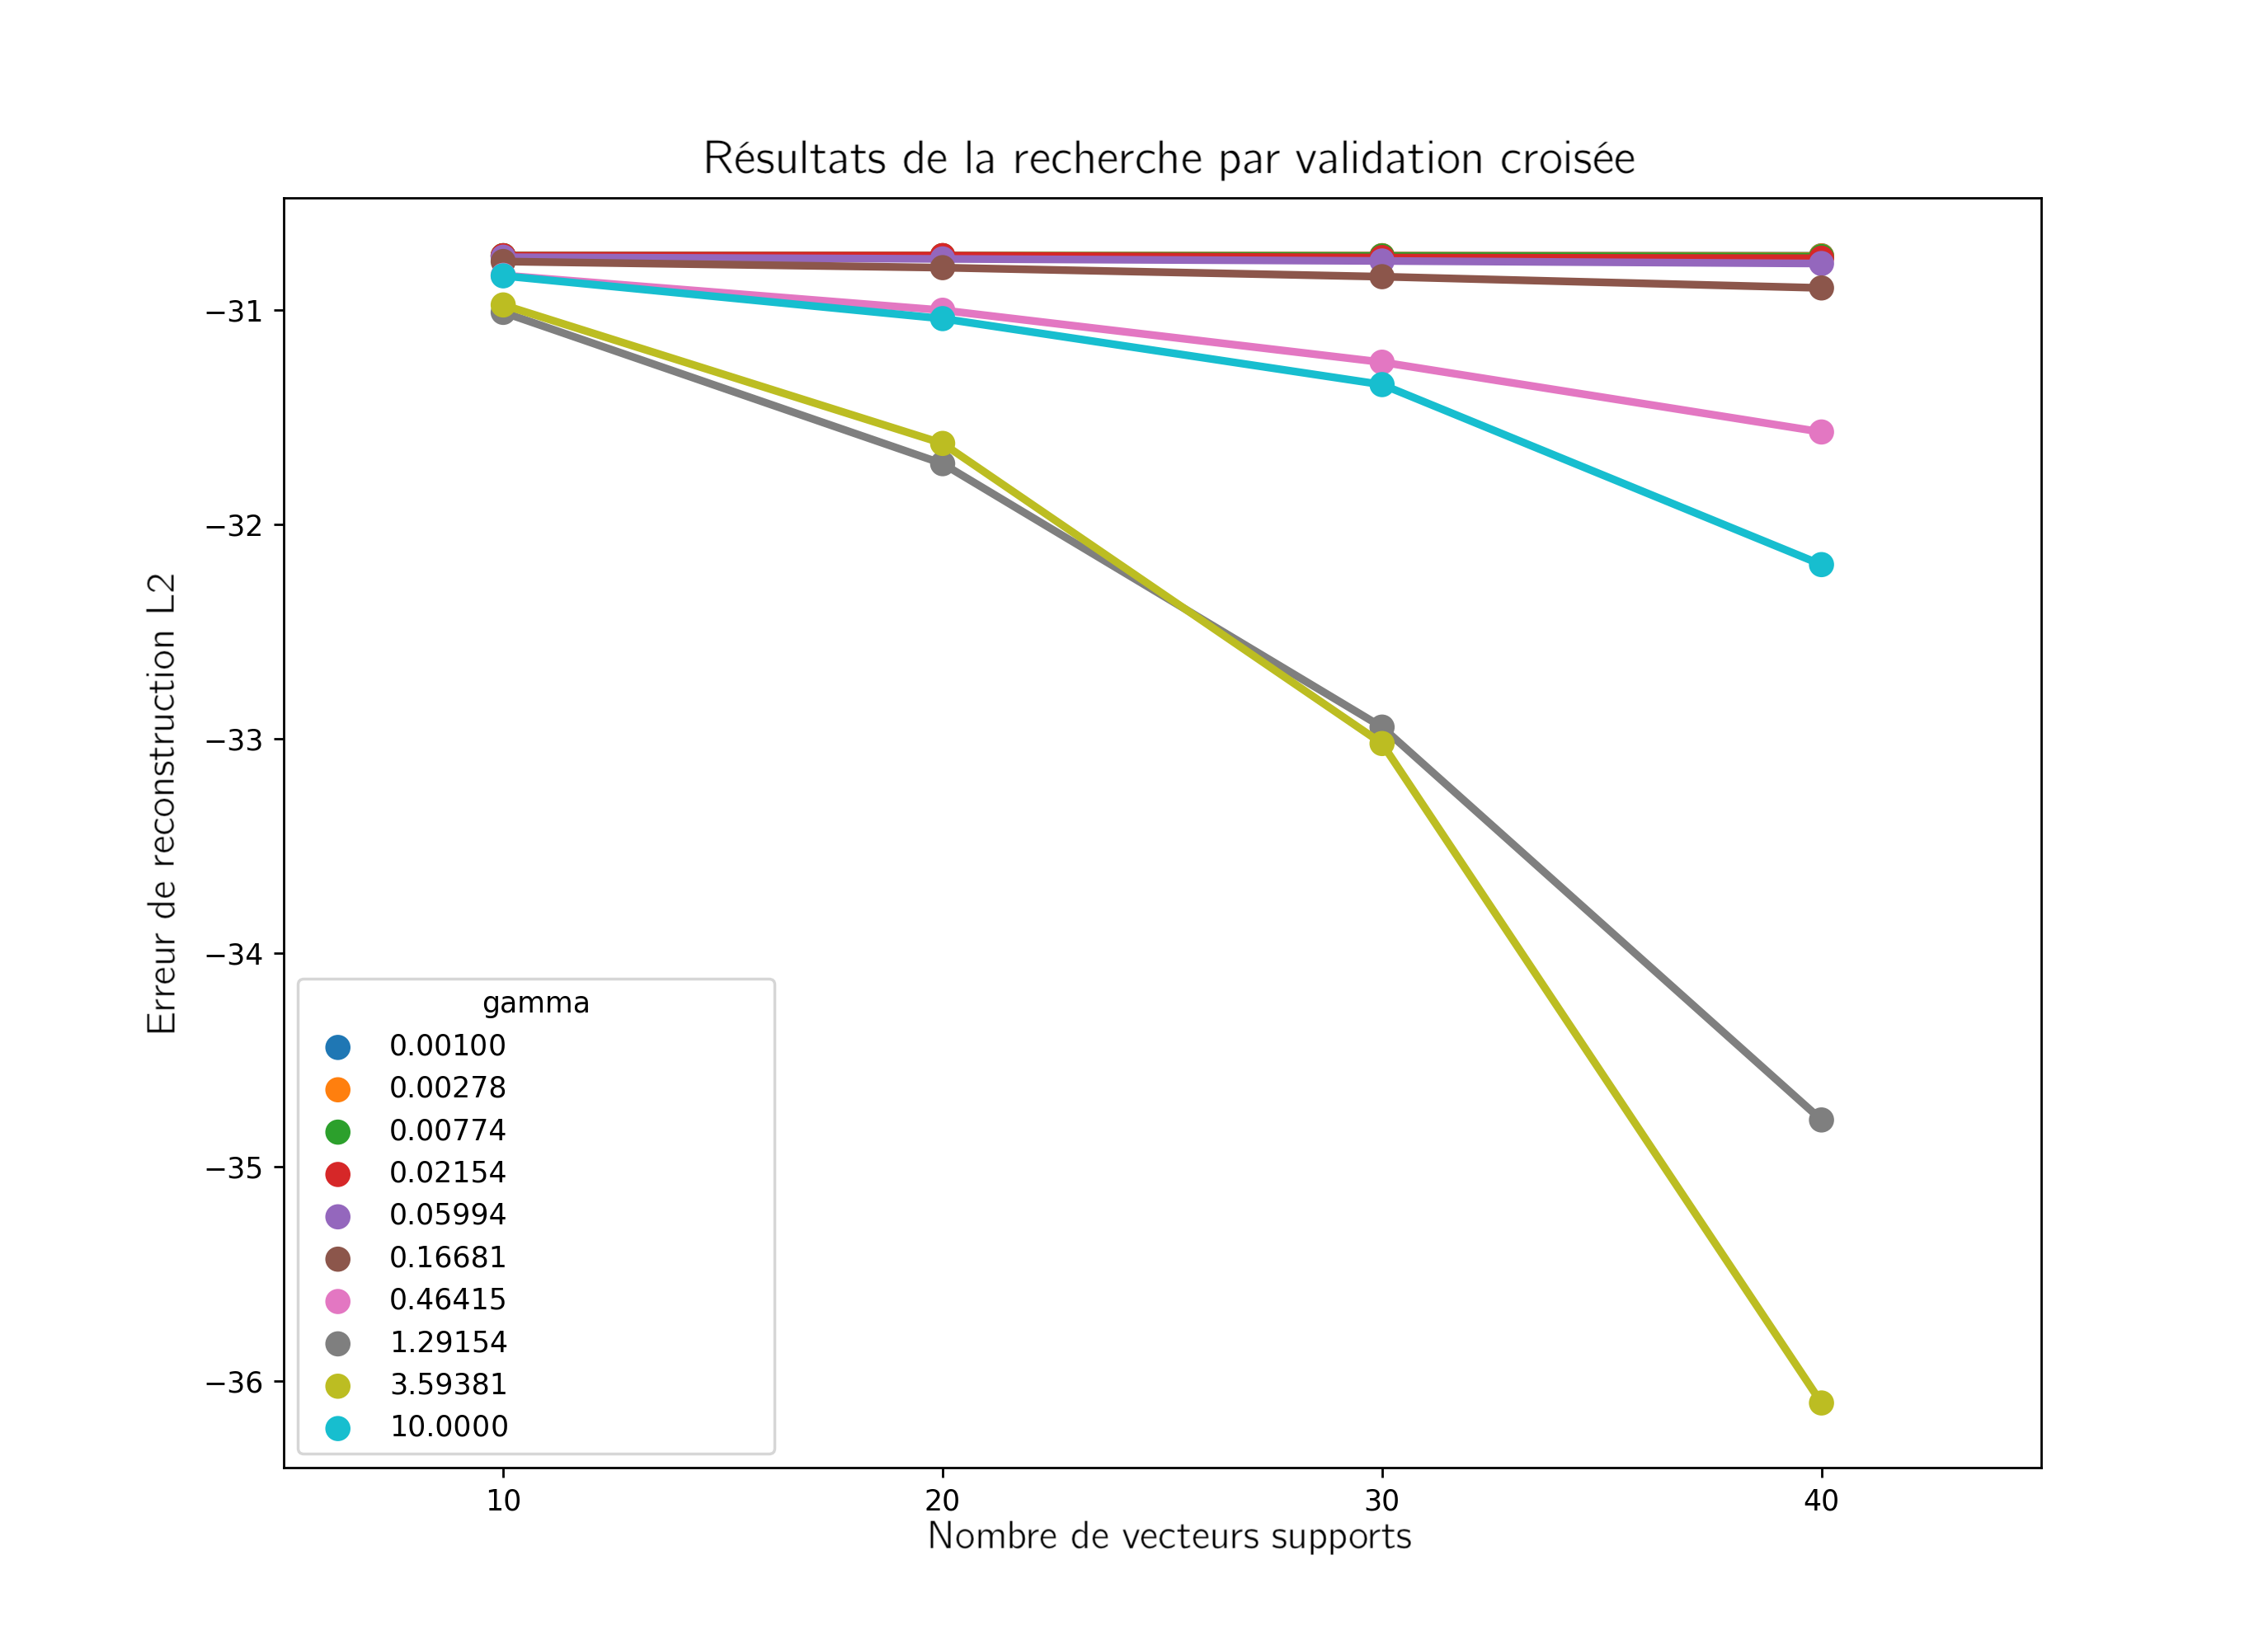
\includegraphics[width=0.95\textwidth,height=0.7\textheight,keepaspectratio]{../Chap4/Figures/KernelPCA_cv_notperf.png}
    \caption{Optimisation des paramètres d'une ACP à noyaux. Métrique : Norme $\ell_{2}$.}
    \label{fig:kernel_pca}
\end{figure}

\begin{figure}[hbtp]
    \centering
    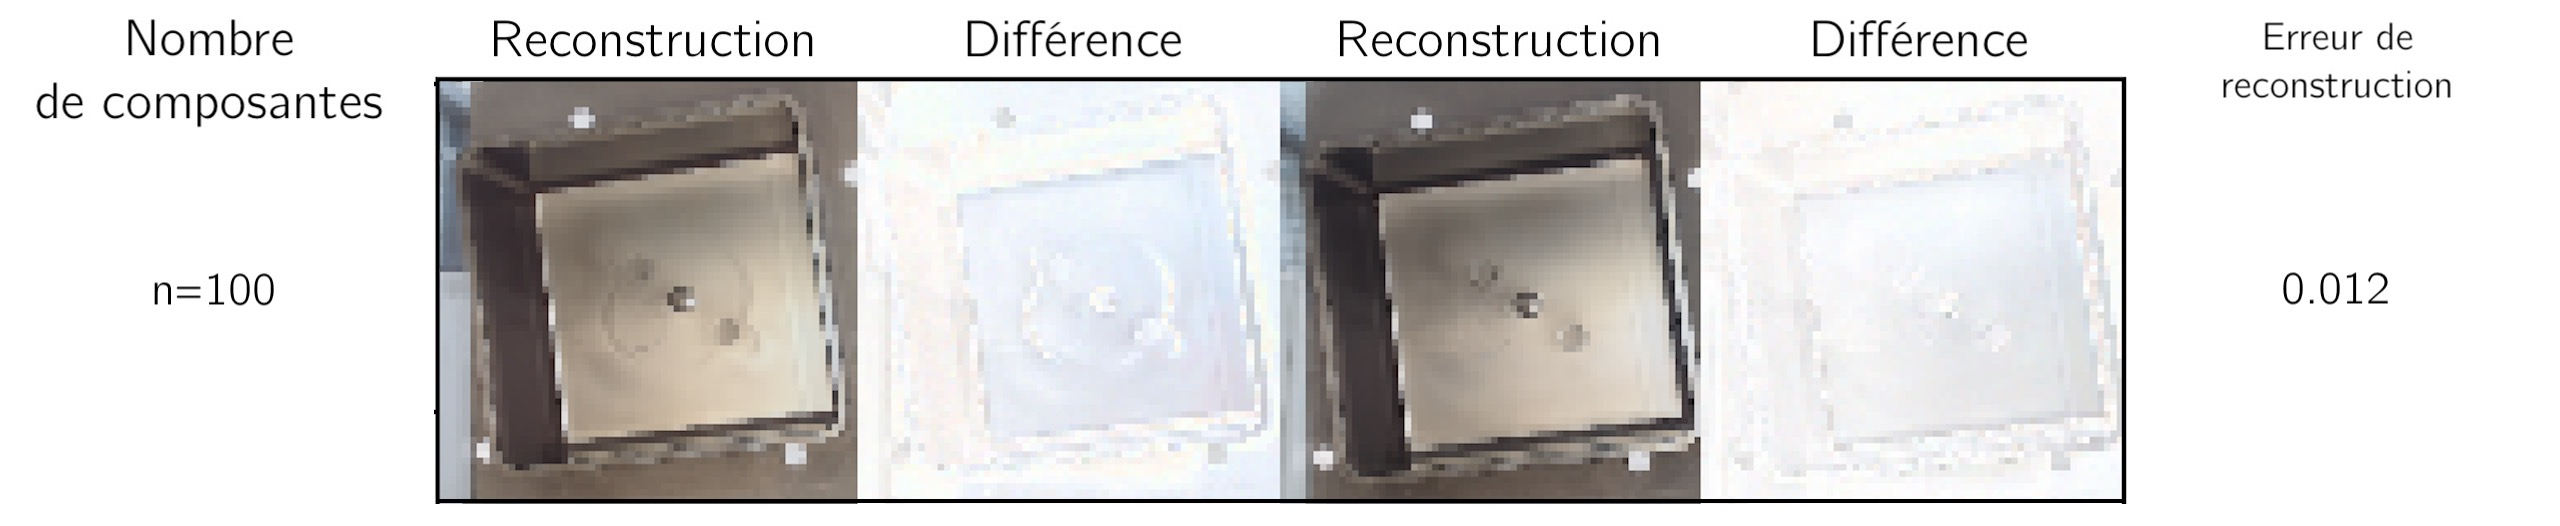
\includegraphics[width=1\textwidth,height=0.7\textheight,keepaspectratio]{../Chap4/Figures/visualize_reconstructed_kPCA100_images.jpg}
    \caption{Compression par ACP à noyau.}
    \label{fig:kpca_reconstruction}
\end{figure}

\begin{figure}[hbtp]
    \centering
    \begin{adjustbox}{width=0.80\textwidth}
        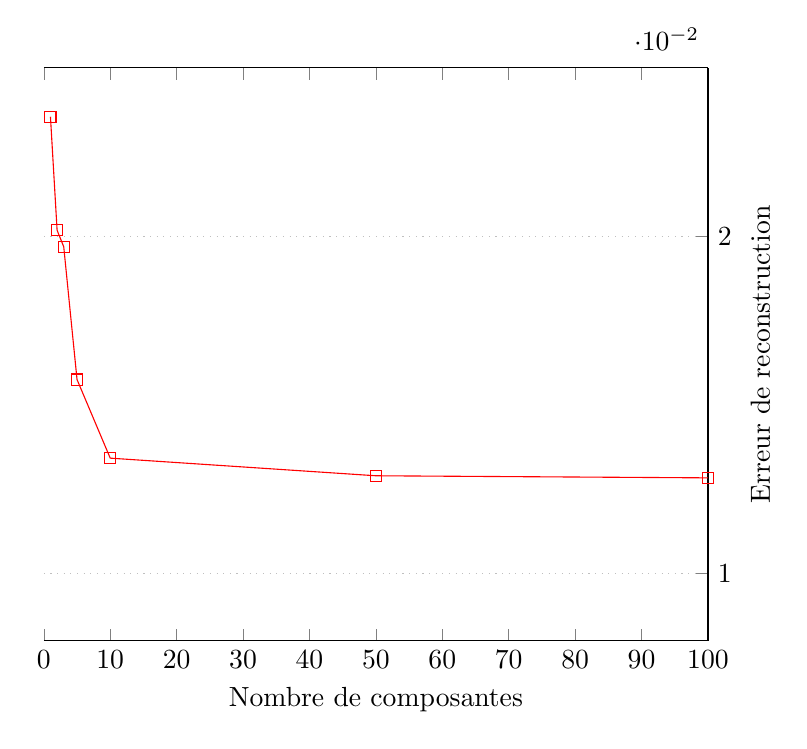
\begin{tikzpicture}
        % let both axes use the same layers
        \pgfplotsset{
            xlabel=x-axis,
            legend columns=-1,
            legend style={draw=none},
            legend to name=named,
        }
        \begin{axis}[
        scale only axis,
        xmin=0, xmax=100,
        axis y line*=right,
        xlabel={Nombre de composantes},
        ylabel style = {align=center},
        ylabel={Erreur de reconstruction}, % \ref{pgfplots:plot1}
        xtick={0,10,20,30,40,50,60,70,80,90,100},
        ymin=0.008, ymax=0.025,
        ytick={0.03,0.02,0.01},
        ymajorgrids=true,
        grid style=dotted,
        ]
        \addplot [color=red,mark=square]
        table{
            1 0.023551
            2 0.020183
            3 0.019691
            5 0.015753
           10 0.013420
           50 0.012897
          100 0.012835
        };
        \addlegendentry{Erreur de reconstruction}, %HINT: should be added on next axis with \addlegendimage
        \label{plot:kpca_mse}
        \end{axis}
        \end{tikzpicture}
    \end{adjustbox}
    \\
    \ref{named}
    \caption{Qualité de la compression par \textit{ACP à noyau} en fonction du nombre de composantes.}
    \label{fig:kpca_plot}
\end{figure}

La Figure \ref{fig:kernel_pca} présente le résultat d'une optimisation sur $k$ : le nombre de paramètres et $\gamma$ : coefficient d'un noyau \textit{RBF}. On choisira ici $k = 20$ et $\gamma = 0,02154$.

Nous obtenons des performances inférieures à l'ACP, Figure \ref{fig:kpca_reconstruction}.
La transformation par un noyau gaussien est ici inutile.
De manière générale, le traitement d'images aux textures complexes nécessite l'utilisation de modèles fortement non linéaires, ce qui n'est pas le cas du noyau gaussien.
C'est pourquoi les méthodes par réseaux de neurones non linéaire obtiennent de meilleurs résultats.
Nous les étudierons dès la section suivante, §\ref{subsubsec:vae}.

La complexité de l'ACP à noyau est $\bigO(m^{2} \cdot n^2+m^{3})$ pour un noyau linéaire et $\bigO(m^{2} \cdot n^3+m^{3})$ pour un noyau gaussien (\textit{RBF}).
Dans le cas $m \ll n$, les complexités sont quadratiques $\bigO(n^2)$ pour un noyau linéaire et cubique $\bigO(n^3)$ pour un noyau gaussien.
Lorsqu'on utilise l'ACP à noyau, on limitera le nombre de variables $m$ des échantillons.
De plus, la difficulté apparait dans le cas où le jeu de données est grand ($n > 1000$) : le coût du stockage du noyau $K$ en mémoire devient significatif.
% Linear SVM $\bigO(N   \cdot m)$
% RBF SVM    $\bigO(N^2 \cdot m)$

\subsubsection{t-SNE} \label{subsubsec:tsne}
% https://scikit-learn.org/stable/modules/clustering.html#spectral-clustering
La méthode \textit{t-SNE} (\textit{t-Distributed Stochastic Neighbor Embedding}) est proposée par \citeauthor{maaten_visualizing_2008} \cite{maaten_visualizing_2008}. C'est une méthode de réduction de l'information itérative particulièrement adaptée à la visualisation des données dans un espace à deux ou trois dimensions.
\textit{t-SNE} est une évolution de la méthode \textit{SNE} (\textit{Stochastic Neighbor Embedding}) \cite{hinton_stochastic_2003}.
Les deux méthodes utilisent la même démarche.
Une distribution de probabilité $P$ est générée afin de modéliser la distribution des distances entre les points, pour le jeu de données initial.
Le nombre de points voisins à prendre en compte est défini par l'hyper-paramètre de \textit{perplexité}.
Une petite valeur de perplexité permet de mettre en évidence les structures locales, alors qu'une grande valeur mettra en évidence les structures globales.
La valeur de perplexité définira la variance de la distribution.
En pratique, on choisira une valeur dans $[5; 50]$.
Une distribution $Q$ est générée afin de modéliser les mêmes propriétés des données, mais dans un espace de dimensions réduites.
On cherche alors à minimiser l'écart entre les deux distributions $P$ et $Q$ afin de trouver la distribution $Q$ optimale.
Cette démarche permet de modéliser la structure non-linéaire des données.
Les paramètres de $Q$ sont ajustés par descente de gradient stochastique, afin de minimiser la divergence de Kullback-Leibler entre les deux distributions, Équation \ref{eq:D_KL}.
\textit{SNE} utilise une distribution de probabilité gaussienne, alors que \textit{t-SNE}, une distribution qui suit une loi de Student (\textit{t-distribution}).
La loi de Student est à queue-longue.
Elle tend plus lentement vers zéro qu'une distribution gaussienne.
Aussi, elle est plus adaptée à la modélisation des distances entre de petits nombres d'échantillons.
Enfin, \textit{t-SNE} propose de simplifier les calculs de l'optimisation de $Q$ en utilisant une loi de Student à un degré de liberté, qui est une loi de Cauchy, $f(t)=\frac{1}{\pi(1+t^2)}$.

Trois conséquences de la méthode limitent son utilisation à la seule visualisation de données.
La réduction de dimensions obtenue n'est pas une fonction.
Aussi, de nouveaux échantillons ne pourront pas être projetées dans l'espace réduit.
L'algorithme est stochastique et chaque exécution produit un résultat différent.
Enfin, les résultats dépendent fortement de la valeur de l'hyper-paramètre \textit{perplexité}.

\begin{figure}[htb]
    \centering
    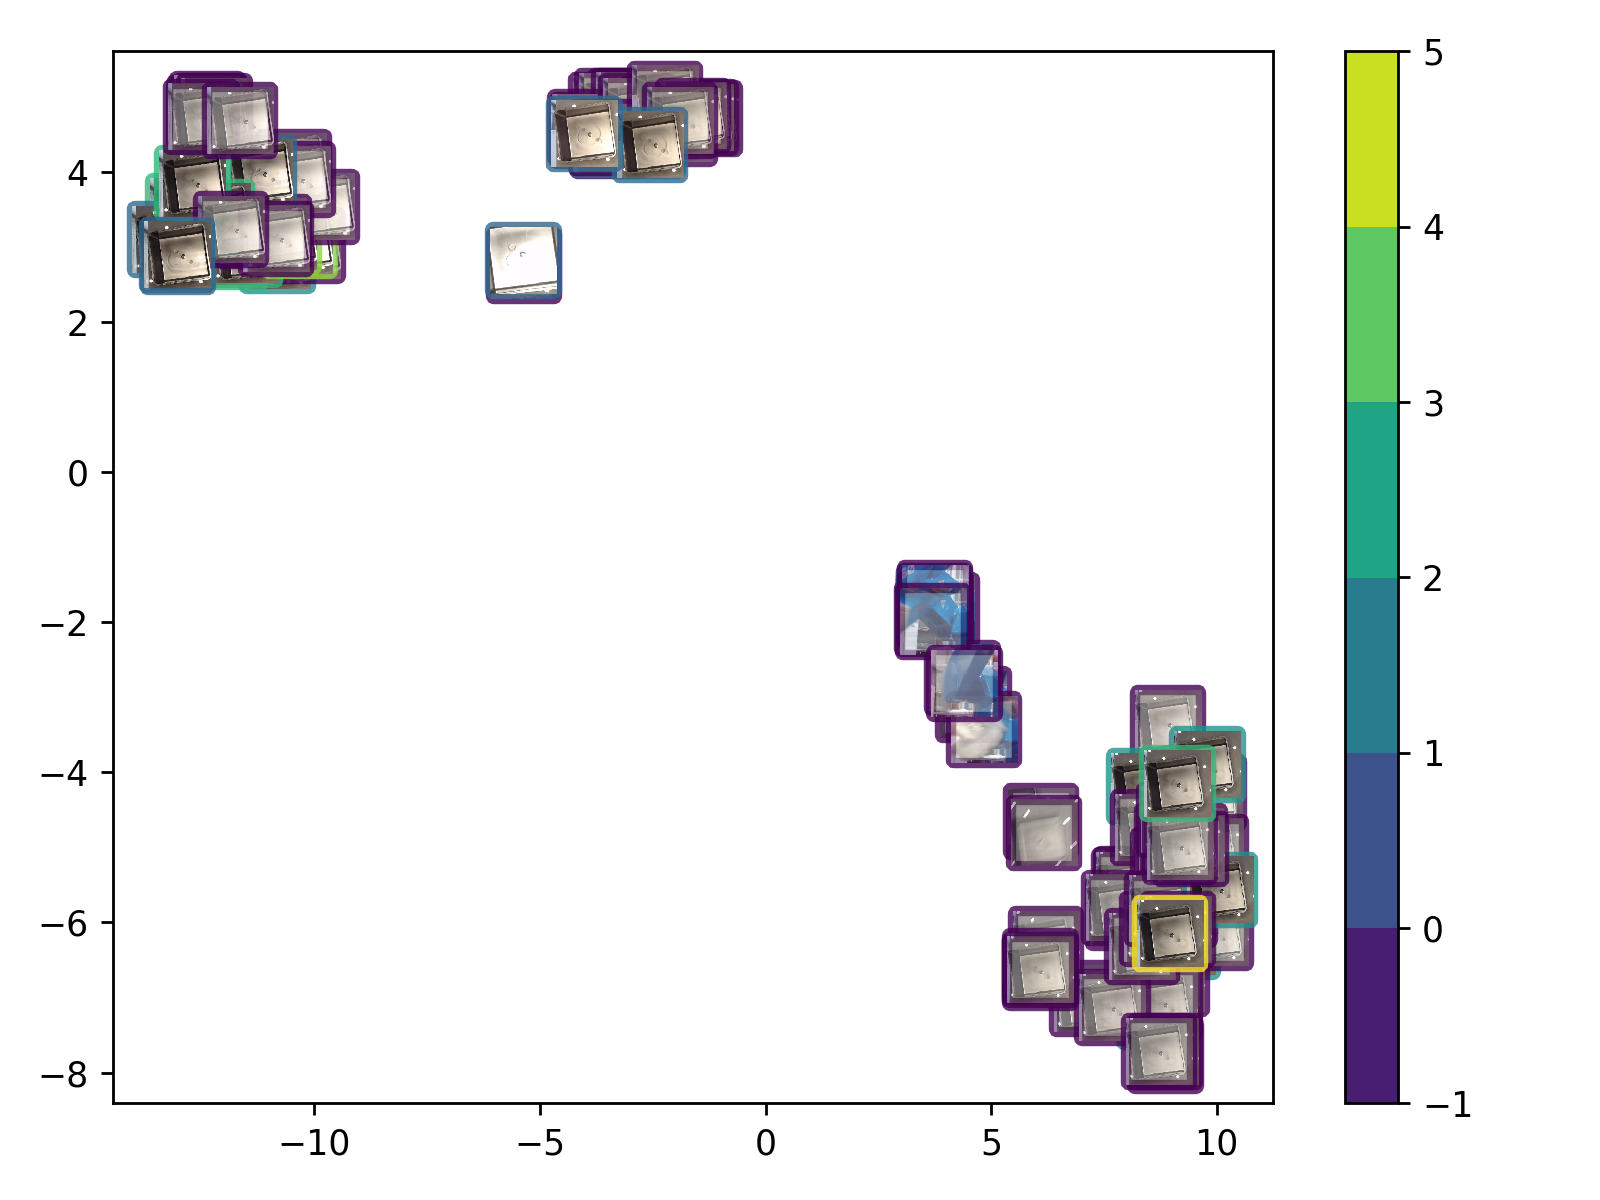
\includegraphics[width=0.95\textwidth,height=\textheight,keepaspectratio]{../Chap4/Figures/visualize_T-SNE_pixel_space.png}
    \caption{Projection par \textit{t-SNE} à partir de la valeur des pixels des images. L'échelle 1-5 correspond aux niveaux de qualité évalués par les experts humains ; -1 correspond aux pièces non annotées.}
    \label{fig:tSNE}
\end{figure}

La Figure \ref{fig:tSNE} présente la projection obtenue par \textit{t-SNE} sur la valeur des pixels bruts de l'image de chaque pièce.
On observe une séparation en quatre paquets, dont un paquet qui contient les images "erronées" (qui ne contiennent pas de pièce).
À la différence de la projection par ACP, Figure \ref{fig:ACP}, trois paquets de différente qualité de pièces sont mis en évidences.
L'algorithme \textit{t-SNE} propose une réduction de dimensions plus pertinente que l'ACP, pour les problèmes où des motifs complexes doivent être distingués.
Cependant, appliquer cet algorithme sur les valeurs des pixels bruts limite les résultats à la séparation de motifs globaux.
Il est nécessaire de réaliser un prétraitement des images pour extraire les motifs pertinents sur notre problème.
Une approche par apprentissage supervisé et réseau de neurones de convolution est la plus pertinente.
L'apprentissage par transfert de domaine (§\ref{subsec:transfer_learning}) peut également être utilisé, comme méthode d'extraction des motifs pertinents.

Une dernière limite de cette méthode est posée par le calcul de la distance Euclidienne entre les points que l'on cherche à modéliser dans les distributions $P$ et $Q$.
La distance Euclidienne nécessite de vérifier l'hypothèse de linéarité de l'espace entre les points.
C'est une hypothèse forte qui est rarement vérifiée pour les données complexes, notamment lorsque la répartition des points n'est pas uniforme.
C'est pourquoi de nouvelles méthodes de réduction de l'information ont été proposées.
Nous nous intéresserons en particulier à la méthode \textit{UMAP} §\ref{subsubsec:umap}, qui utilise la géométrie riemannienne pour résoudre ces limites.

La complexité de l'algorithme t-SNE est de l'ordre de $\bigO(d N^2)$, avec $d$ la dimension de l'espace réduit.
\cite{maaten_accelerating_2014} propose d'accélérer l'algorithme à une complexité de $\bigO(d N \log N)$, dans le cas où $d \le 3$ en approximant le gradient par l'algorithme à arbres binaires de recherche de \citeauthor{barnes_hierarchical_1986} \cite{barnes_hierarchical_1986}.

\subsubsection{UMAP} \label{subsubsec:umap}
La méthode de réduction de l'information \textit{UMAP} est proposée par \citeauthor{mcinnes_umap_2018} \cite{mcinnes_umap_2018, mcinnes_umap_2018a}.
Elle s'appuie sur l'apprentissage de variété (\textit{manifold learning}).
On cherche, dans l'espace de dimensions initiales, une variété (des surfaces topologiques), pour laquelle les données sont au plus proche de celle-ci.

La variété obtenue est alors une représentation des données dans un espace de dimensions réduites.
Alors que l'ACP réalise une projection dans un espace euclidien, \textit{UMAP} projette les données dans un espace riemannien.
L'espace riemannien possède les hypothèses de connexité et de complétude, ce qui limite la perte d'informations.
L'algorithme \textit{UMAP} cherche une variété $\mathbb{V}$ dans cet espace, telle que les données soient situées au plus proches de celle-ci.
Afin d'utiliser cette démarche, trois hypothèses sont faites :
\begin{itemize}
\item La distribution des données est uniforme sur la variété $\mathbb{V}$ utilisée.
\item La métrique riemannienne peut être localement approximée comme une constante.
\item L'espace riemannien utilisé est connexe.
\end{itemize}

Le théorème du nerf \cite{zisman_topologie_1972} affirme qu'il est possible de représenter la variété topologique $\mathbb{V}$ par un n-simplexe\footnote{Un simplexe est l'élément topologique le plus simple possible.}.
% https://ncatlab.org/nlab/show/nerve+theorem
% K. Borsuk, On the imbedding of systems of compacta in simplicial complexes , Fund. Math 35, (1948) 217-234
% J. Leray. Sur la forme des espaces topologiques et sur les points fixes des représentations. J. Math. Pures Appl. 24:95–167, 1945
Dans ce cas, $\mathbb{V}$ et sa représentation en simplexes sont équivalentes.
Il est alors possible de modéliser ces simplexes par une distribution combinatoire $P$, en appliquant la logique floue (topologie-floue).
Nous invitons le lecteur qui souhaite approfondir ce raisonnement à consulter la publication originale des auteurs de l'algorithme \textit{UMAP} \cite{mcinnes_umap_2018}.
Par la suite, représenter les données dans un espace de petites dimensions, revient à trouver la variété de petites dimensions qui possède la distribution $Q$ la plus similaire possible, avec la distribution $P$ de la variété des données initiales.
Cela revient à trouver la distribution $Q$ telle que l'entropie croisée entre les deux distributions $P$ et $Q$ soit minimale.
Cette démarche est similaire à la minimisation de la divergence de Kullback-Leibler de \textit{t-SNE} §\ref{subsubsec:tsne} qui met en évidence la structure locale des données, mais elle permet également de préserver la structure globale.
% -> I am using the UMAP for Dimensionality Reduction. It's implementation really bods well with my data. I have a question regarding the feature importance. Suppose, after the dimensionality reduction, the UMAP separates out the labels clearly and creates the 3 subgroups containing all labels. Can I somehow get the list of features corresponding to each group? Which features were more relevant to which group?
% -> One option that I have seen done is to build a classifier based on the clusters and then use SHAP or LIME to get interpretations of what separates the clusters.

\begin{figure}[hbtp]
    \centering
    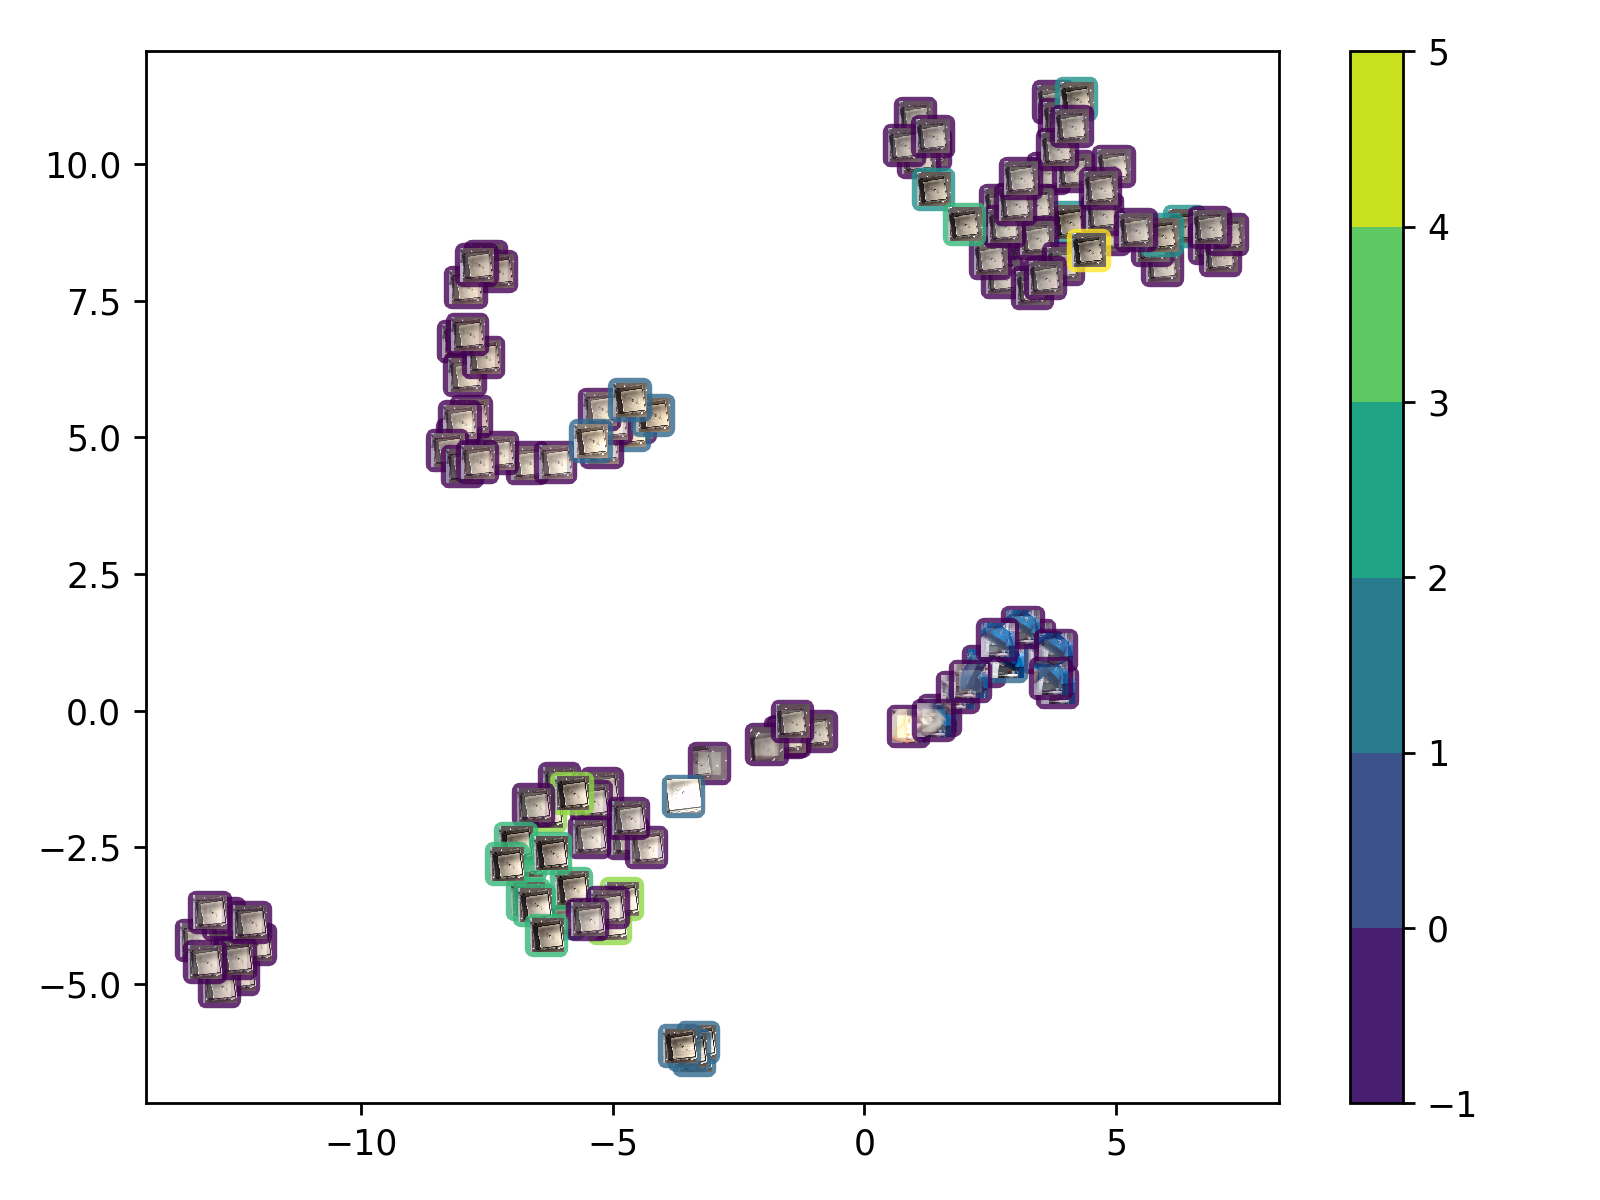
\includegraphics[width=\textwidth,height=\textheight,keepaspectratio]{../Chap4/Figures/visualize_UMAP_pixel_space.png}
    \caption{Représentation par \textit{UMAP} à partir de la valeur des pixels des images. L'échelle 1-5 correspond aux niveaux de qualité évalués par les experts humains ; -1 correspond aux pièces non annotées.}
    \label{fig:umap}
\end{figure}

La Figure \ref{fig:umap} présente la représentation en deux dimensions obtenues en appliquant \textit{UMAP} sur la valeur des pixels brutes de l'image.
En comparaison de \textit{t-SNE}, \textit{UMAP} permet de mettre en évidence la structure globale des données dans les deux dimensions, tout en conservant la structure locale des paquets d'échantillons.
Les images qui ne contiennent pas de pièces sont séparées, ainsi que le paquet de pièces annotées d'un niveau de qualité 0 (mauvais).
De plus, le niveau de qualité 1 est séparé.
Les niveaux 2 à 5 sont représentés dans deux paquets distincts.
Il apparait un paquet de pièces de très bonne qualité (niveau 5).
Ce paquet contient quelques pièces des niveaux 3 et 4 ; aussi cela indique que l'annotation humaine n'est pas robuste lorsque l'on approche de la qualité maximale.
En comparaison des résultats obtenus avec un réseau de triplets, Figure \ref{fig:triplet_result}, cette méthode présente une séparation des paquets identiques, mais sans annotation humaine et avec un coût de calcul plus de cent fois moindre.
L'approche topologique permet d'améliorer les performances et la méthode \textit{UMAP} montre son intérêt dans le cadre d'une approche non-supervisée de suggestion d'annotation à l'expert humain.

Afin de trouver le graphe de la représentation en petites dimensions, \textit{UMAP} utilise l'algorithme (\textit{Nearest-Neighbor-Descent}) d'optimisation de graphes proposé par \citeauthor{dong_efficient_2011} \cite{dong_efficient_2011}.
Les auteurs évaluent empiriquement la complexité de leur méthode de l'ordre de $\bigO(N^{1.14})$.
Aussi, la complexité de la méthode \textit{UMAP} est limitée par cet algorithme.
Elle est de l'ordre de $\bigO(N \log N)$.

% ivis: structure preserving dimensionality reduction
% https://bering-ivis.readthedocs.io/en/latest/

\subsubsection{Auto-encodeurs variationnels} \label{subsubsec:vae}.
Un auto-encodeur cherche à reproduire la donnée entrée, avec le minimum de paramètres (ou Degrés De Liberté).
Aucune annotation des données n'est requise.
C'est une méthode qui permet d'apprendre la représentation des données dans un espace de dimensions réduites (aussi appelé \textit{feature learning} ou \textit{representation learning}).
En 1987, \citeauthor{lecun_modeles_1987, gallinari_memoires_1987} proposent un réseau auto-encodeur utilisant des réseaux de neurones, afin de supprimer le bruit d'images \cite{lecun_modeles_1987, gallinari_memoires_1987}.
Dans leurs travaux, ils étudient la capacité du réseau à mémoriser les caractéristiques des images initiales, en fonction de son architecture.
En parallèle, \citeauthor{ballard_modular_1987} propose un auto-encodeur (appelé dans ce texte \textit{systèmes auto-associatifs}) à trois couches \cite{ballard_modular_1987}.
Dans ces travaux, les poids des neurones sont ajustés par rétro-propagation du gradient, qui a été récemment proposée.

Un auto-encodeur se compose de deux parties : un encodeur $z = f(x)$ qui compresse l'information initiale dans un espace de dimensions réduites (appelé \textit{espace latent}) et un décodeur $\hat x = g(z)$ qui reconstruit ensuite une approximation de $x$ à partir de $z$.
$f$ et $g$ sont généralement des réseaux de convolutions profonds, dont les poids respectifs sont $\mathbf{W}_f$ et $\mathbf{W}_g$.
La Figure \ref{fig:autoencoder_architecture} présente l'architecture d'un auto-encodeur qui utilise des réseaux de convolutions pour ces fonctions.

\begin{figure}[hbtp]
    \centering
    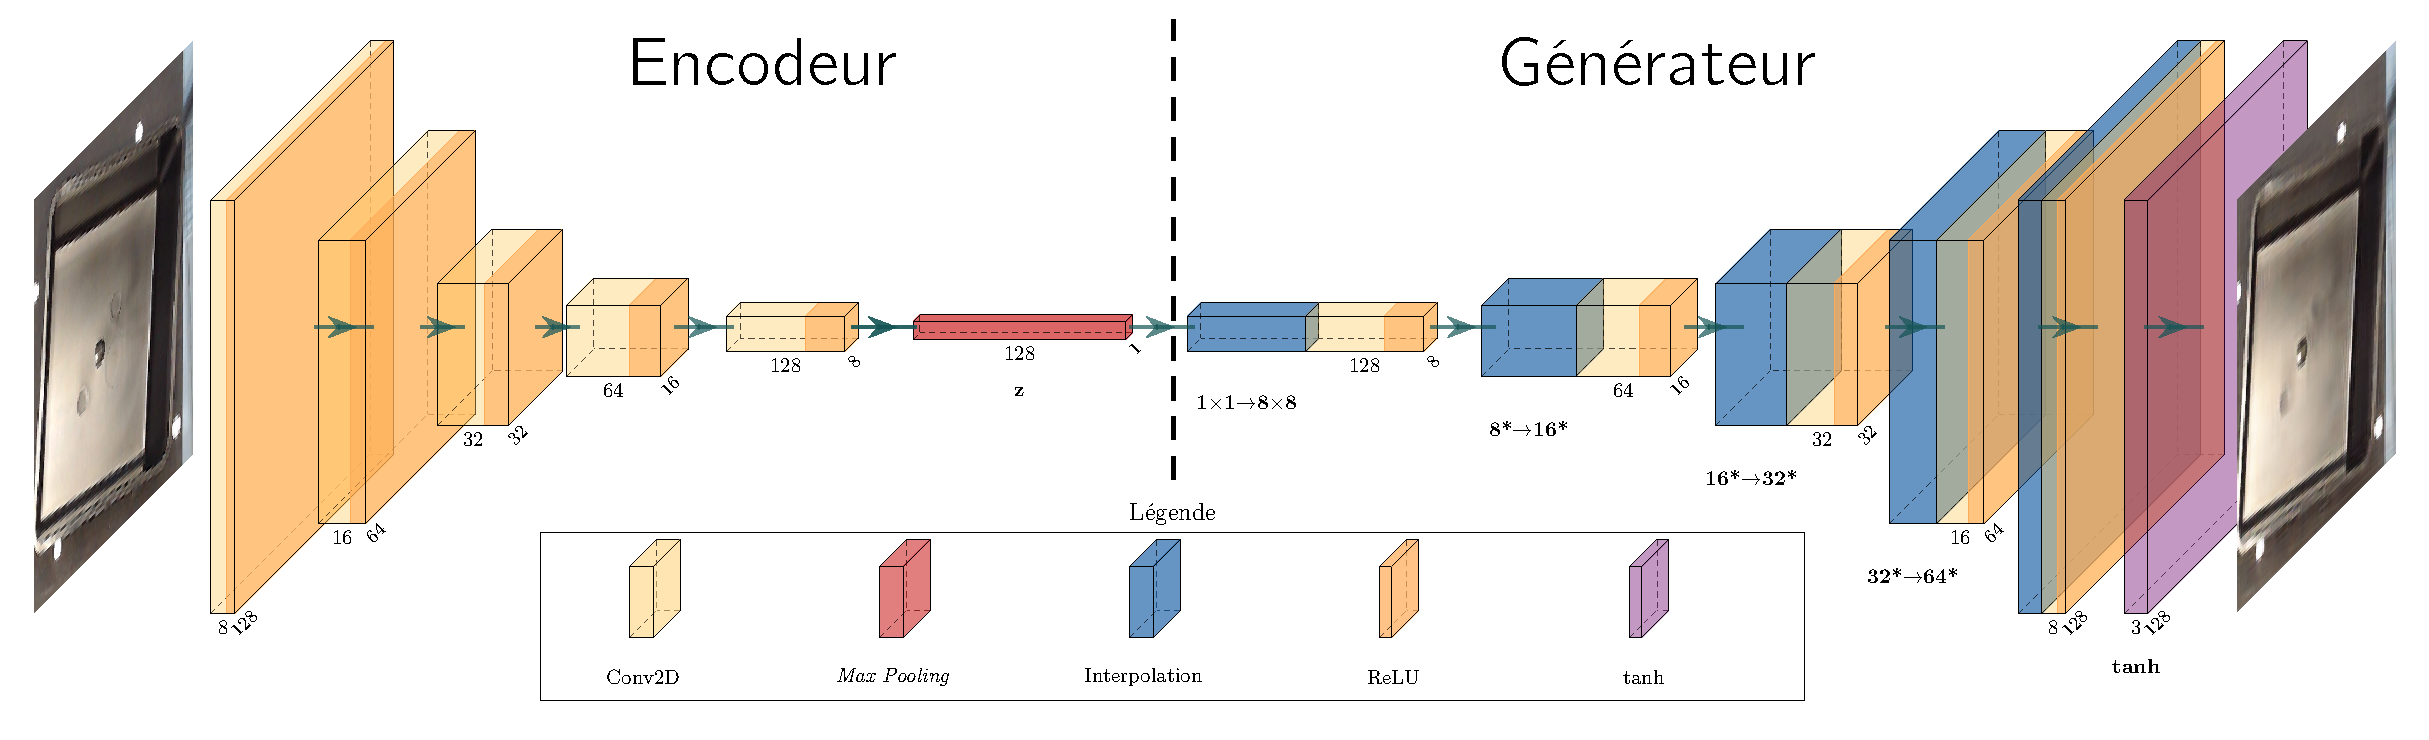
\includegraphics[width=\textwidth,height=\textheight,keepaspectratio]{../Chap4/Figures/autoencoder_architecture.pdf}
    \caption{Architecture d'un auto-encodeur.}
    \label{fig:autoencoder_architecture}
\end{figure}

Afin de mesurer la similitude telle que $x \simeq \hat x$, la fonction de coût à minimiser lors de l'apprentissage du modèle est souvent l'erreur quadratique entre $x$ et $\hat x$, Équation \ref{eq:autoencoder}.

\begin{equation} \label{eq:autoencoder}
\min _{\mathbf{W}_{f}, \mathbf{W}_{g}} \mathcal{L}_{g\acute{e}n\acute{e}ration}\left(x, \hat{x}\right) = \min _{\mathbf{W}_{f}, \mathbf{W}_{g}} \left\|x-g\left(f\left(x, \mathbf{W}_{f}\right), \mathbf{W}_{g}\right)\right\|_{2}^{2}
\end{equation}

Enfin, une contrainte indispensable est appliquée à la dimension de $z$, qui doit être très petite devant la dimension de $x$.
Ainsi, seules les propriétés les plus importantes des données sont prises en compte.
Un cas particulier apparait si le décodeur $g$ est une application linéaire et si la fonction de coût est l'erreur quadratique : alors les valeurs de $z$ sont équivalentes aux valeurs propres d'une Analyse en Composante Principale \cite{bourlard_autoassociation_1988}.

La Figure \ref{fig:autoencoder} présente une image entrée et sa reconstruction après le passage dans un auto-encodeur dont $z$ a une dimension de 128 valeurs.
On observe la perte d'information visuelle : la marque de l'éjecteur a, par exemple, disparu.
En revanche, les défauts d'aspect qui nous intéressent sont reproduits.
Le taux de compression est ici de 120 : $124 \times 124$ pixels $\rightarrow 128$ valeurs.
À la différence de la compression par ACP, Figure \ref{fig:pca_reconstruction}, la reconstruction ne possède pas d'artefacts.
En revanche, le coût de calcul de cette méthode est beaucoup plus grand que pour une ACP.
Il est nécessaire de disposer d'une accélération des calculs massivement parallèle, par exemple sur processeur graphique, pour pouvoir construire un modèle à partir d'un grand nombre d'échantillons.

\begin{figure}[hbtp]
    \centering
    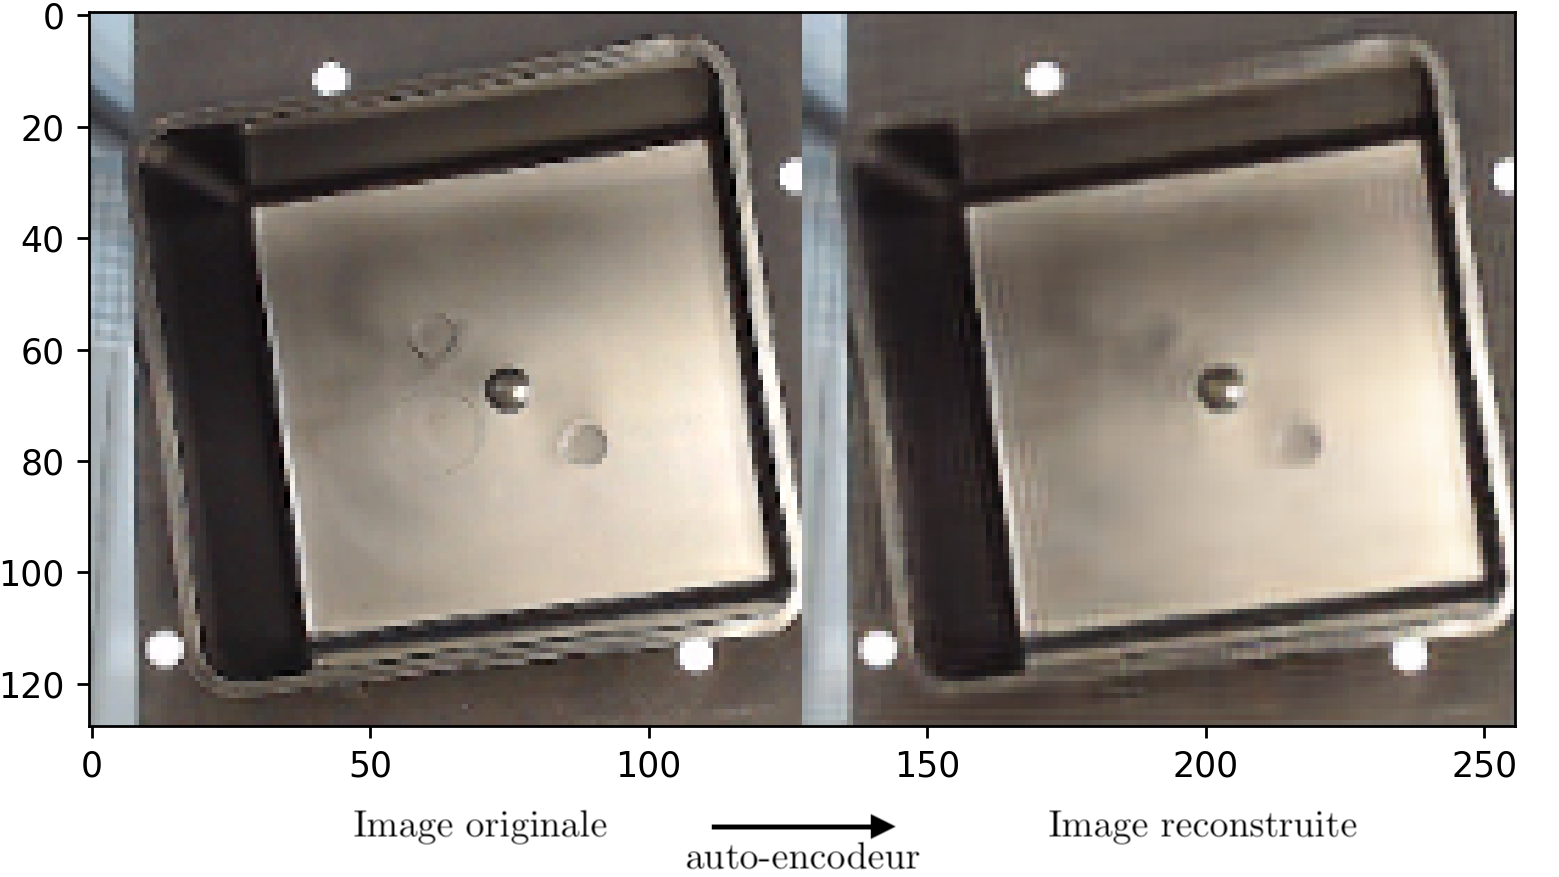
\includegraphics[width=0.75\textwidth,height=\textheight,keepaspectratio]{../Chap4/Figures/visualize_reconstructed_variations.png}
    \caption{Reconstruction d'une image par un auto-encodeur.}
    \label{fig:autoencoder}
\end{figure}

La Figure \ref{fig:tSNE_ae} présente les valeurs des 128 dimensions de $z$ projetées par l'algorithme \textit{t-SNE}, présenté dans la Section \ref{subsubsec:tsne}.
Les différentes classes exprimées dans l'espace latent $z$ sont mieux séparées que dans la Figure \ref{fig:tSNE} qui utilisait les données brutes : l'ensemble des valeurs des pixels.
On observe également que l'évaluation des cinq classes de qualité, évaluées par les experts humains, est respectée.
Les pièces non annotées sont positionnées dans les bonnes classes.
Enfin, il est intéressant d'observer qu'un paquet correspondant à une erreur de mesure, comme par exemple l'absence de pièces et la capture du bras robotique préhenseur est mis en évidence.

\begin{figure}[hbtp]
    \centering
    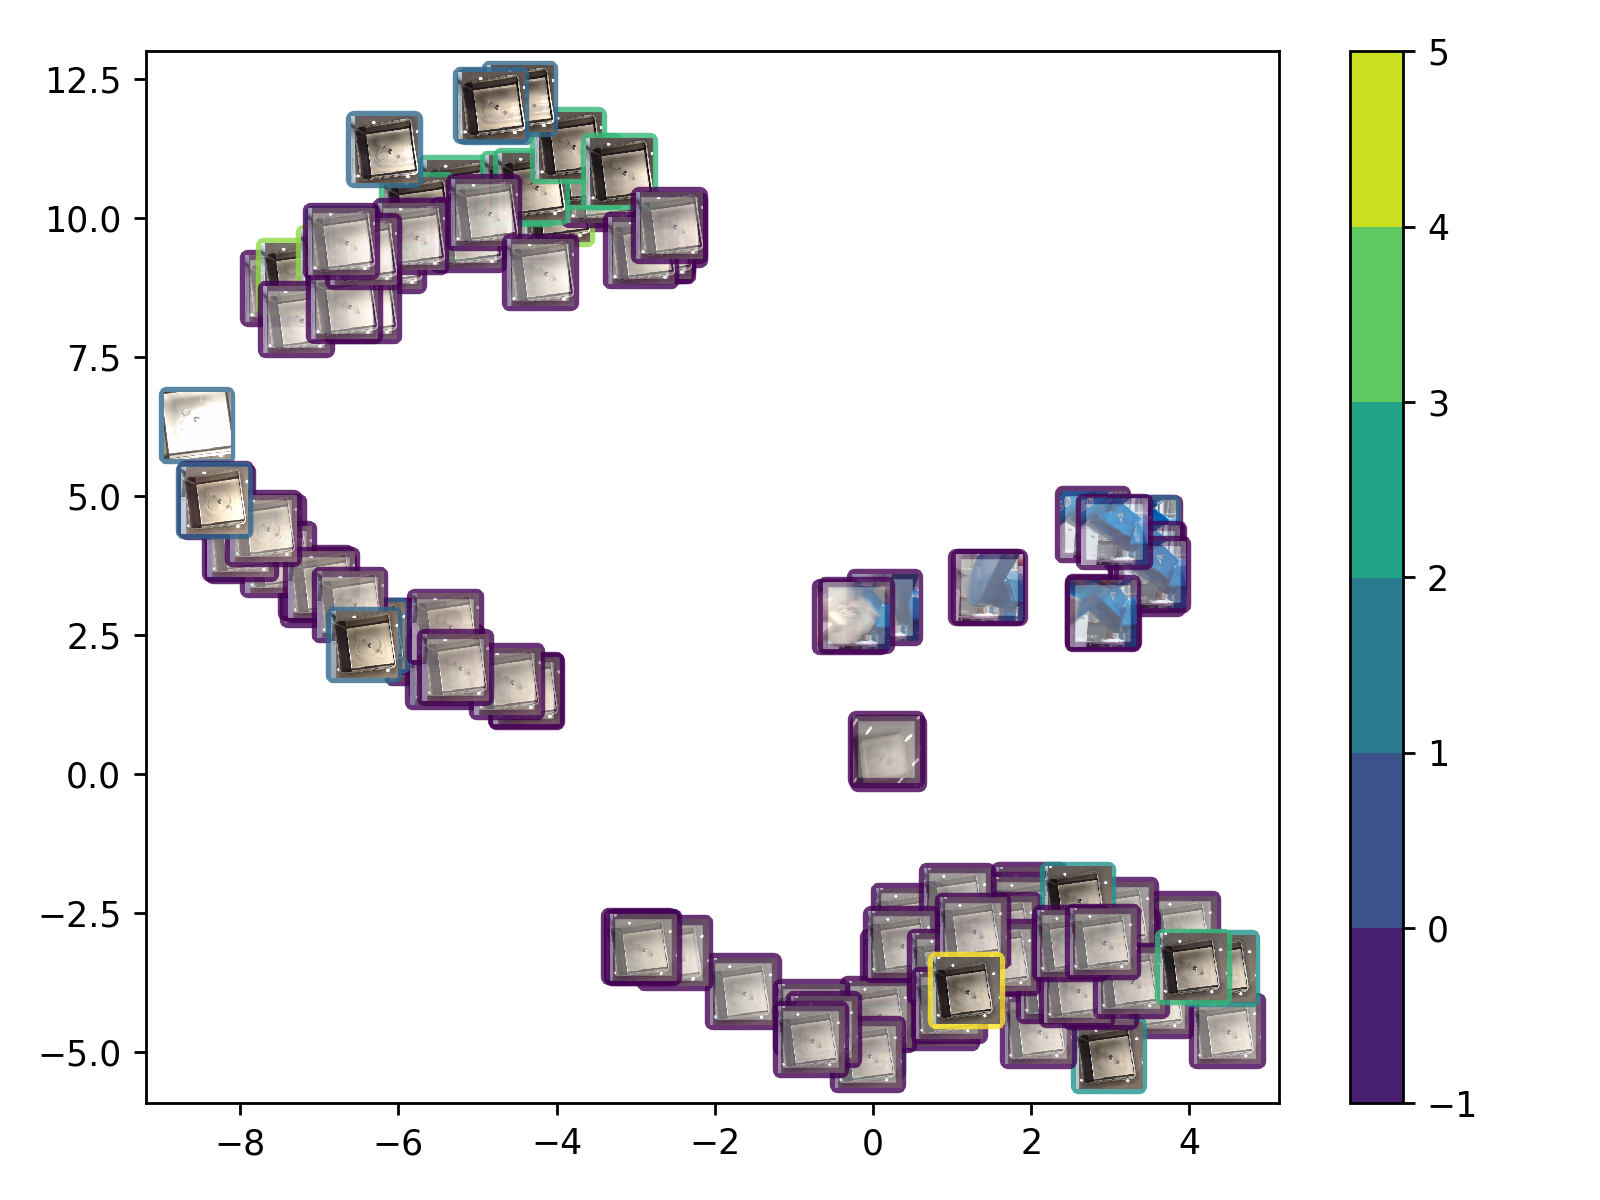
\includegraphics[width=0.95\textwidth,height=\textheight,keepaspectratio]{../Chap4/Figures/visualize_T-SNE_latent_space.png}
    \caption{Projection par \textit{t-SNE} à partir des valeurs de l'espace latent $z$ d'un \textit{VAE}. L'échelle 1-5 correspond aux niveaux de qualité évalués par les experts humains ; -1 correspond aux pièces non annotées.}
    \label{fig:tSNE_ae}
\end{figure}

% Séparabilité des classes
% Neighborhood Hit score
% Fernando Vieira Paulovich, Luis Gustavo Nonato, Rosane Minghim, and Haim Levkowitz. Least square projection: A fast high-precision multidimensional projection technique and its application to document mapping. IEEE Trans. Vis. Comput. Graph., 14(3):564–575, 2008
% http://cedric.cnam.fr/vertigo/Cours/ml2/tpDeepLearning4.html#exercice-3-separabilite-des-classes-et-representations-internes-des-reseaux-de-neurones

Un auto-encodeur modélise une application (encodeur $x \rightarrow z$) et l'application inverse (générateur $z \leadsto \hat x$).
Cependant, il est difficile d'interpoler les valeurs de $z$ afin de générer des $\hat x$, car l'espace $z$ n'a pas de contrainte de continuité ; aussi $z$ est généralement discontinue.
Récemment, l'auto-encodeur variationnel (\textit{Variational Auto-Encoder}) est proposé par \citeauthor{kingma_autoencoding_2013, rezende_stochastic_2014} \cite{kingma_autoencoding_2013, rezende_stochastic_2014}.
Il utilise une méthode d'inférence variationnelle.
À la différence d'un auto-encodeur, un VAE modélise le générateur $g$ sous la forme d'une distribution de probabilité $p(x | z)$ sur les données.
De même, l'encodeur $f$ sera une distribution $q(z | x)$.
Un a priori fort sur la distribution $q$ est introduit : on cherche généralement $q(z | x)$ qui soit proche d'une gaussienne centrée $\mathcal{N}(\mu=0,\sigma=1)$.
Ainsi, $q$ sera continue.
Cette condition revient à minimiser la divergence de Kullback-Leibler entre la distribution de l'encodeur $q(z | x)$ et la distribution du générateur $p(z | x)$.
L'auto-encodeur variationnel nécessite une fonction de coût composite, Équation \ref{eq:vae}.

\begin{equation} \label{eq:vae}
\begin{split}
\mathcal{L}_{VAE} = \mathcal{L}_{g\acute{e}n\acute{e}ration} + \mathcal{L}_{latent}
\\
\text{avec } \mathcal{L}_{latent}\left(\hat{y}, y\right) = Divergence_{K L}\left(p(z | x) \| N(\mu=0 ; \sigma=1)\right)
\end{split}
\end{equation}

\begin{figure}[hbtp]
    \centering
    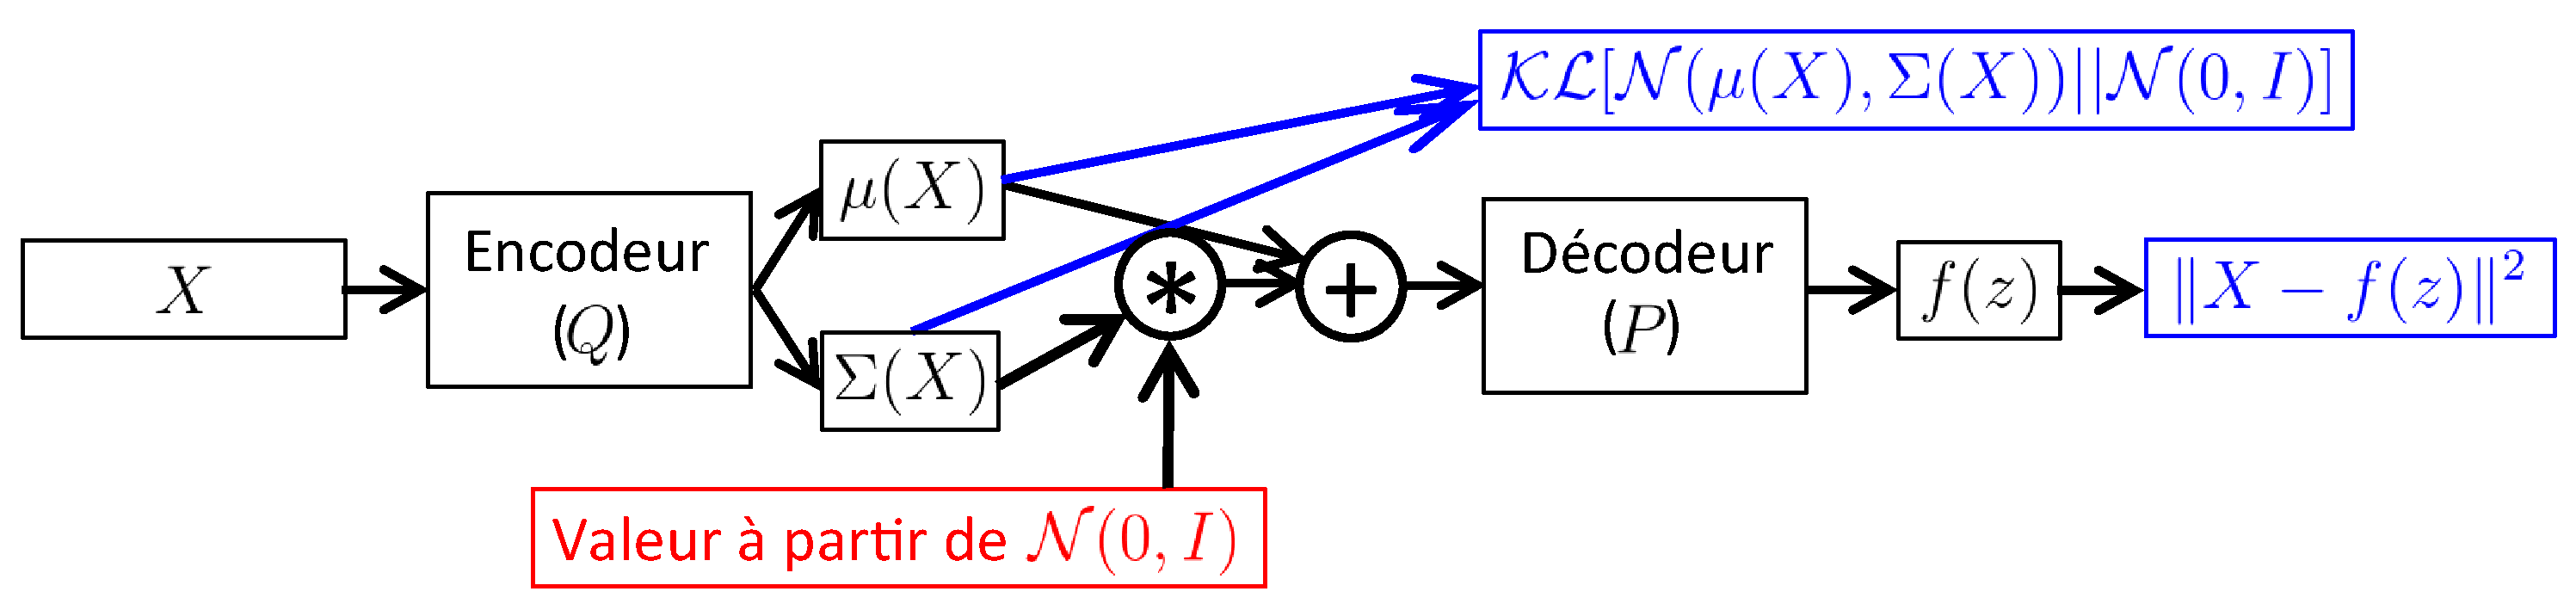
\includegraphics[width=\textwidth,height=\textheight,keepaspectratio]{../Chap4/Figures/vae_from_Doersh2016.pdf}
    \caption{Graphe d'un auto-encodeur variationnel, inspiré de \cite{doersch_tutorial_2016}.}
    \label{fig:vae}
\end{figure}

Lors de l'apprentissage, les distributions $p$ et $q$ sont modélisées par des réseaux de neurones.
Les sorties du générateur seront les paramètres de la distribution : la moyenne et l'écart-type, tels que $q(z | x) = \mathcal{N}\left(z ; \vec{\mu}(x), \operatorname{diag}(\vec{\sigma}(x))^{2}\right)$.
La Figure \ref{fig:vae}, inspirée de \cite{doersch_tutorial_2016}, représente le graphe de calcul de ce modèle.
Il devient possible de générer de nouvelles sorties à partir de la distribution $p(z)$, en tirant les valeurs de $z$ à partir de la distribution $\mathcal{N}(\mu=0,\sigma=1)$.
Ces nouvelles sorties ne sont pas nécessairement similaires aux données d'apprentissages de $x$.
Ainsi, l'auto-encodeur variationnel généralise l'auto-encodeur et le rend \textit{génératif}.

\begin{figure}[hbtp]
    \centering
    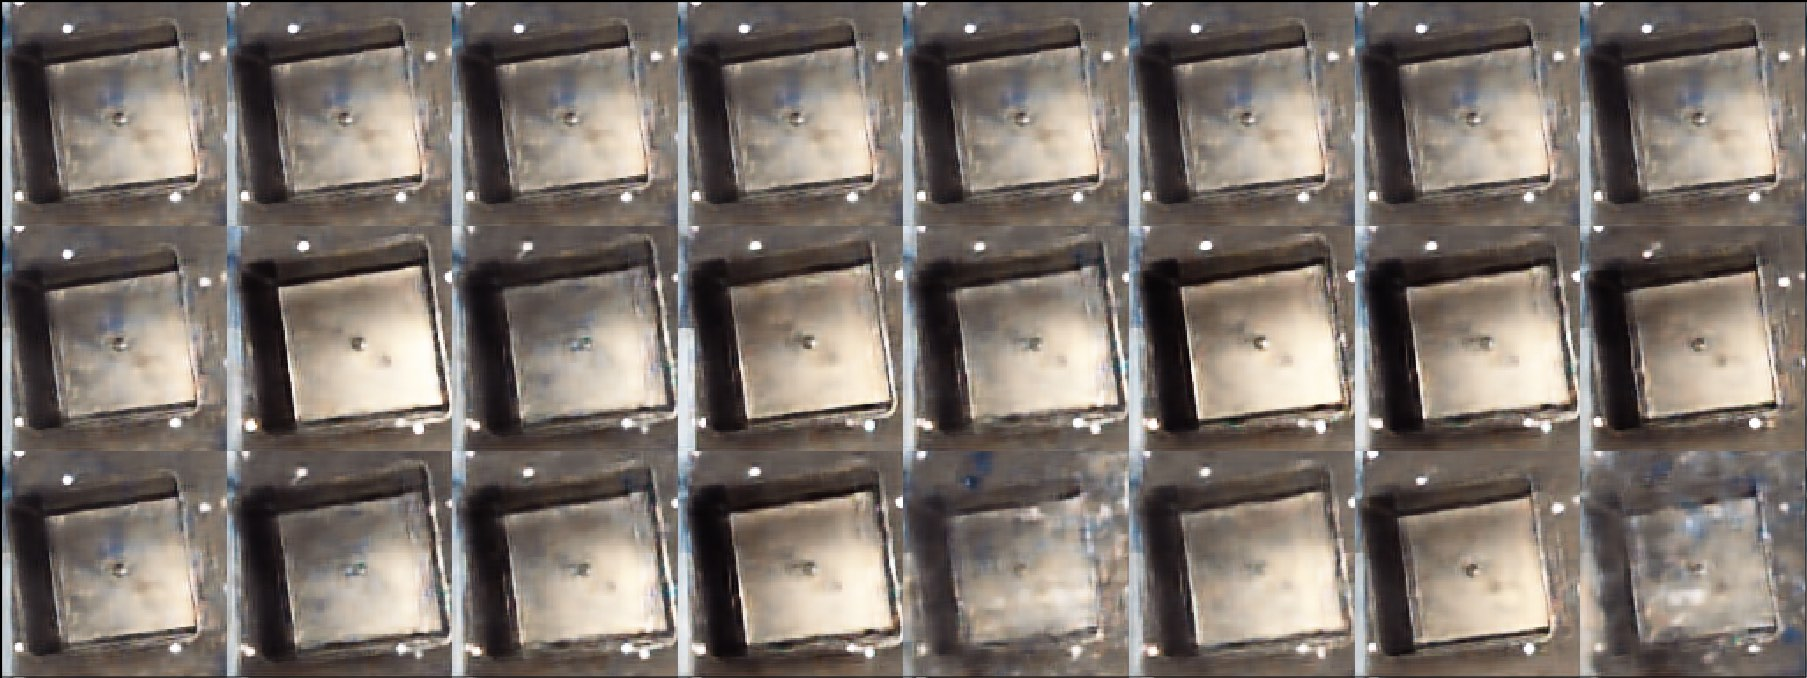
\includegraphics[width=\textwidth,height=\textheight,keepaspectratio]{../Chap4/Figures/visualize_interpolations_latent.jpg}
    \caption{Génération d'images à partir de la distribution modélisant l'espace latent d'un auto-encodeur variationnel.}
    \label{fig:vae_sampling}
\end{figure}

La Figure \ref{fig:vae_sampling} montre des images générées à partir de tirages aléatoires sur la distribution $P$ de l'espace latent $z$.
On observe la diversité des défauts modélisés dans $z$, mais également le réalisme limité que produit le générateur d'un VAE.
Cela est dû à la compression élevée et au petit jeu de données dont nous disposons ce qui entraine du bruit.
Il est intéressant d'observer des artefacts de couleur bleu, qui correspondent à la présence d'images dans le jeu de données où il n'y pas de pièce, mais où le bras robotique de couleur bleue est présent.
Le bras robotique est néanmoins très peu présent dans $z$ en comparaison des pièces : le VAE est robuste.

Les réseaux génératifs permettent de palier de manière intéressante au manque de variétés des échantillons dans les petits jeux de données.
Cependant, les images générées sont souvent floues, ce qui est souvent dû à la fonction de coût, l'erreur moyenne entre $x$ et $\hat x$, utilisée lors de l'apprentissage.
En effet, l'erreur moyenne ne permet pas la prise en compte dans $z$ des motifs complexes qui sont peu présents dans le jeu de données.
Dernièrement, \citeauthor{kingma_introduction_2019} \cite{kingma_introduction_2019} propose une synthèse exhaustive des solutions à cette problématique : construire des modèles plus profonds, ajouter des contraintes plus pertinentes dans la fonction de coût, comme par exemple des tâches de classification auxiliaires, et mettre à jour de manière plus judicieuse les poids lors de l'apprentissage du modèle.
Un autre type de modèle génératif propose également d'améliorer le réalisme des images générées.
L'apprentissage n'est pas réalisé sur l'erreur entre $x$ et $\hat x$, mais de manière indirecte à partir de la valeur retournée par un second modèle.
Ce principe permet d'améliorer le réalisme en prenant en compte des motifs complexes lors de la reconstruction.
Il s'agit des modèles antagonistes génératifs que nous détaillons dans la Section \ref{subsubsec:GAN}.

L'apprentissage d'un modèle VAE est réalisé par descente de gradient stochastique.
Les poids du modèle sont ajustés sur un sous-ensemble du jeu de données de taille $B$ échantillons (appelé mini-batch), pendant $T$ itérations.
La complexité de l'apprentissage est de l'ordre de $\bigO(T B^2 D + T B^2 d)$, avec $T$ le nombre d'itérations, $B$ le nombre d'échantillons dans un mini-batch, $D$ la dimension d'un échantillon et $d$ la dimension de l'espace latent.
De plus, la quantité de mémoire de travail nécessaire au stockage des mini-batch est de l'ordre de  $\bigO(B^2 D)$.
Ces coûts de calcul sont importants.
Dans nos expériences, c'est la quantité de mémoire de travail sur le processeur graphique dont nous disposons (11 Giga octets) qui conditionne le nombre d'échantillons par mini-batch (ici, $B=64$ et $D=128^2$), d'où la complexité des calculs ($T=100$, $B=64^2$, $D=128^2$). Nous obtenons une complexité de l'ordre de 7 Milliards d'opérations et une occupation mémoire de l'ordre de 10 Giga octets.
La durée de l'apprentissage de notre modèle VAE est d'une heure sur un processeur graphique dédié (\textit{NVIDIA GTX 1080 Ti}).
Avec les ressources informatiques actuelles, une mise à jour journalière de ce modèle peut être envisagée, lors de son utilisation au sein d'un procédé industriel.

% Great ressources on AE & VAE:
% https://www.deeplearningbook.org/contents/generative_models.html
% https://ermongroup.github.io/cs228-notes/extras/vae/
% http://anotherdatum.com/vae.html
% http://anotherdatum.com/vae2.html
% http://anotherdatum.com/vae-moe.html
% https://arxiv.org/abs/1606.05908 Tutorial on Variational Autoencoders
% Diederik P. Kingma PhD thesis: Variational inference & deep learning: A new synthesis
% https://bjlkeng.github.io/posts/variational-autoencoders/
% https://bjlkeng.github.io/posts/a-variational-autoencoder-on-the-svnh-dataset/
% http://www.cs.toronto.edu/~urtasun/courses/CSC2541_Winter17/Deep_generative_models.pdf
% Adversarial Autoencoders arXiv:1511.05644
% Bayesian NN http://anotherdatum.com/bnn.html

% \cite{kingma_semisupervised_2014}
% https://bjlkeng.github.io/posts/semi-supervised-learning-with-variational-autoencoders/
% https://github.com/bjlkeng/sandbox/tree/master/notebooks/vae-semi_supervised_learning
% Auxiliary Deep Generative Models https://arxiv.org/abs/1602.05473
% One-shot: Danilo Jimenez Rezende, Shakir Mohamed, Ivo Danihelka, Karol Gregor, and Daan Wierstra. One-shot generalization in deep generative models. arXiv preprint arXiv:1603.05106, 2016b.

% ELBO surgery https://rachitsingh.com/elbo_surgery/
% Fixing a broken ELBO https://lyusungwon.github.io/generative-models/2018/06/29/fbe.html

% https://arxiv.org/abs/1906.00446, Generating Diverse High-Fidelity Images with VQ-VAE-2, June 2019

% Nous proposons l'architecture suivante : split_coef doit être un diviseur de 1920 et un carré parfait : [1, 4, 16, 32, 64]

\subsubsection{Réseaux antagonistes génératifs} \label{subsubsec:GAN}
Proposés par \citeauthor{goodfellow_generative_2014} \cite{goodfellow_generative_2014}, les réseaux antagonistes génératifs (\textit{Generative Adversarial Networks}) permettent de raffiner le modèle de l'espace latent.
En comparaison avec les auto-encodeurs, les images issues du générateur sont plus proches des images originales.
Les \textit{GAN} s'appuient sur une association de deux modèles qui sont entrainés en concurrence : un générateur $g$ génère $\hat x = g(z)$ et un classifieur $d$ (appelé \textit{discriminateur}) calcule la probabilité $p$ que $\hat x$ appartienne au jeu de donnée réel, $p = d(x)$.
L'objectif du générateur est de générer $\hat x$ tel que $\hat x \simeq x$, tandis que l'objectif du discriminateur est de distinguer les $\hat x$ générés par le générateur, des $x$ réels, issues du jeu de données initial.
La phase d'apprentissage de ce modèle est similaire à un duel de la théorie du jeu où le générateur et son adversaire le discriminateur s'affrontent.
Les deux modèles sont entrainés en parallèle afin d'apprendre les poids $w_g$ et $w_d$ qui maximiseront leurs performances.
Un équilibre de Nash \cite{nash_equilibrium_1950, nash_noncooperative_1951} est théoriquement atteint lorsque le générateur produit des $\hat x$ qui ne peuvent plus être distingués des $x$ par le discriminateur.
Trouver le générateur $g$ optimal revient à résoudre le problème d'optimisation de l'Équation \ref{eq:GAN} pour toute donnée d'entrée $x$.
Cependant, comme le problème d'optimisation cherche à minimiser un terme et minimiser un autre terme, la solution optimale est difficile à obtenir lors de l'ajustement des poids par descente de gradients stochastique car de nombreux optimums locaux (optimum pour un seul des membres) existent \cite{goodfellow_generative_2014}.

\begin{equation} \label{eq:GAN}
g_{optimal}  = \min _{g} \max _{d} = \mathbb{E}_{\mathbf{x} \sim p_{\text { réelle }}} \log d(\boldsymbol{x})+\mathbb{E}_{\boldsymbol{x} \sim p_{\text { générée }}} \log (1-d(\boldsymbol{x}))
\end{equation}

Le modèle \textit{GAN} fait partie des nombreux modèles proposés depuis les années 1990, qui s'appuient sur un apprentissage non-supervisé par affrontement de deux modèles qui s'opposent dans un jeu de minimisation-maximisation.
\citeauthor{schmidhuber_unsupervised_2019} propose une revue des travaux fondateurs sur le sujet \cite{schmidhuber_unsupervised_2019}.
Le dynamisme actuel de la littérature sur les modèles de type \textit{GAN}, ainsi que la disponibilité des implémentations ouvertes par leurs auteurs, nous a permis d'évaluer ces modèles sur notre problématique.
De nombreux modèles utilisant des idées proches restent à évaluer.
Ils pourraient permettre d'obtenir de meilleures performances sur notre problématique d'analyse de la qualité des produits.

À la suite de la proposition originale des \textit{GAN}, \citeauthor{radford_unsupervised_2015} \cite{radford_unsupervised_2015} proposent des règles pour adapter les \textit{GAN} à la reconstruction d'images : remplacer les couches de moyenne (\textit{pooling}, §\ref{parag:pooling}) par des convolutions de noyaux $1 \times 1$, utiliser la normalisation de lot \ref{parag:batchnorm}, ne pas utiliser de couches pleinement connectées, utiliser l'activation \textit{ReLU} \ref{subsubsec:activation} pour le générateur sauf pour la dernière couche \textit{tanh}, utiliser \textit{LeakyReLU} pour le discriminateur et enfin des règles de construction de l'architecture du réseau qu'ils nomment \textit{DCGAN}.
Ce travail évalue ces règles avec comme objectif d'encoder des jeux de données d'images complexes dans un espace latent de dimensions 100.
Enfin, le travail montre l'intérêt des \textit{GAN} pour réaliser une classification d'images de manière non-supervisée (pas d'annotation des données d'apprentissage).
Il s'agit d'utiliser le générateur comme fonction d'extraction des valeurs pertinentes d'une image (espace latent), puis ensuite d'utiliser un classifieur \textit{SVM} \ref{parag:svm} sur ces dimensions de l'espace latent.
Les performances sont légèrement inférieures à celles obtenues par une approche supervisée, ce qui montre l'intérêt de la méthode puisqu'il n'a pas été nécessaire d'annoter les données pour obtenir ce résultat.
Le \textit{GAN}, puisqu'il est entrainé pour reconstruire une image à partir des dimensions réduites de l'espace latent, permet également d'extraire l'information pertinente des images.
Cette approche est particulièrement intéressante et nous chercherons à l'utiliser afin de répondre aux problèmes industriels où les jeux de données sont petits.

Par la suite, \citeauthor{salimans_improved_2016} \cite{salimans_improved_2016} complètent les règles du modèle \textit{DCGAN}.
\citeauthor{odena_semisupervised_2016, salimans_improved_2016} \cite{odena_semisupervised_2016, salimans_improved_2016} proposent en parallèle de réaliser l'apprentissage de manière semi-supervisée.
L'objectif est de créer un discriminateur qui soit également capable de répondre au problème de classification d'un jeu de données annotées.
Il s'agit d'introduire dans le jeu de données annotées une nouvelle classe "image générée".
Pour un jeu de données comportant $K$ classes, on obtient un jeu de données de $K+1$ classes.
On utilise alors le générateur pour produire les images correspondant à cette nouvelle classe $K+1$.
Cette démarche est alors introduite dans la fonction de coût du discriminateur, Équation \ref{eq:GAN_semisup}.
Ainsi, on obtient un discriminateur qui répond au problème de classification supervisée, tout en étant capable de distinguer les images générées par le générateur.
L'intérêt est double : augmentation artificielle du jeu de données et robustesse aux échantillons adversaires (les "fausses" images générées).
% arXiv:1804.09170v4 Realistic Evaluation of Deep Semi-Supervised Learning Algorithms 

\begin{equation} \label{eq:GAN_semisup}
g_{optimal}  = \min _{g} \max _{d} = \mathbb{E}_{\mathbf{x} \sim p_{\text { réelle }}} \log d(\boldsymbol{x})+\mathbb{E}_{\boldsymbol{x} \sim p_{\text { générée }}} \log (1-d(\boldsymbol{x}))
\end{equation}

Par la suite, des améliorations importantes sont apportées à la méthode.
\citeauthor{arjovsky_wasserstein_2017} \cite{arjovsky_wasserstein_2017} proposent de modifier la fonction de coût du discriminateur qui évalue la qualité de la reconstruction en utilisant la distance de Wasserstein.
\cite{gulrajani_improved_2017}, ainsi que la normalisation spectrale \cite{miyato_spectral_2018}.

L'ensemble de la littérature évalue les performances de ces modèles sur la base de données \textit{ImageNet}.
En comparaison, dans notre cas d'application, le nombre de classes est très faible, de deux classes à une dizaine de classes : pour représenter une échelle qualité bonne — qualité mauvaise, ou pour représenter différentes typologies de défauts.
C'est pourquoi un réseau génératif simple est capable de réaliser une synthèse fidèle des nos images.
En revanche, sur une base de données qui comporte une grande variété de classes, comme \textit{ImageNet}, il apparait que les modèles génératifs ne permettent pas de modéliser les associations entre des éléments géométriques qui doivent nécessairement être présents dans les images d'une classe.
Un exemple est celui de la représentation d'un chien, auquel la texture de pelage est bien appliquée par le modèle \textit{GAN}, mais qui ne possède pas quatre pattes attachées au corps.
%https://lilianweng.github.io/lil-log/2018/06/24/attention-attention.html
Cette limite provient de l'opérateur de convolution qui est une opération locale spatialement contrainte.
Par exemple, l'opérateur de convolution ne peut pas associer la valeur du pixel située en haut à gauche, avec celle en bas à droite.
De plus, lors de l'ajustement des poids par rétro-propagation du gradient, il n'y a pas de relation spatiale entre la valeur en sortie de convolution et les valeurs en entrées.
Cette problématique est critique dans le domaine du traitement de textes et la traduction (\textit{Natural Language Processing}) : la sémantique d'une phrase dépend de la position des mots dans la phrase.
% Also, Neural Turing Machines, by Alex Graves, Greg Wayne, Ivo Danihelka, Oct 2014, https://arxiv.org/abs/1410.5401
C'est pourquoi le mécanisme d'\textit{attention} a été proposé par \citeauthor{bahdanau_neural_2014} \cite{bahdanau_neural_2014} pour la traduction de texte, puis étendu à l'analyse d'images par un réseau de convolutions par \cite{xu_show_2015}.
Par la suite, \citeauthor{vaswani_attention_2017} \cite{vaswani_attention_2017} propose l'architecture de couche \textit{transformer}, qui généralise la méthode en éliminant l'usage de réseaux récurrents.
% http://www.peterbloem.nl/blog/transformers
Ils montrent qu'un réseau constitué uniquement de couches d'\textit{attention} permet d'atteindre les performances de l'état de l'art en traduction de texte.
L'\textit{attention} est depuis utilisée dans toutes les méthodes de l'état de l'art en traduction automatique.
Une couche d'\textit{attention} pondère la valeur d'entrée par une distribution de probabilité, dont les paramètres sont appris, et qui dépend de la position spatiale de la valeur entrée.
Cette démarche est similaire aux portes d'activations des réseaux \textit{LSTM}, ainsi qu'à l'architecture des \textit{Highway Networks}, §\ref{subsubsec:ResNet}, §\ref{eq:highway}.

Dernièrement, \citeauthor{zhang_selfattention_2018} \cite{zhang_selfattention_2018} propose le modèle \textit{SAGAN} (\textit{Self-Attention Generative Adversarial Networks}) qui associe l'utilisation de multiples méthodes et introduit l'utilisation du mécanisme d'\textit{attention}.
Il s'agit pour la couche d'\textit{attention} de modéliser une relation de dépendance pour un pixel, entre tous les autres pixels.
Il n'y a ainsi plus de restriction spatiale aux convolutions.

% https://towardsdatascience.com/not-just-another-gan-paper-sagan-96e649f01a6b
% https://xlnwel.github.io/blog/deep%20learning/SAGAN/
% Spatial transformer Jaderberg et al., 15, is not rly transformer/attention

\begin{figure}[hbtp]
    \centering
    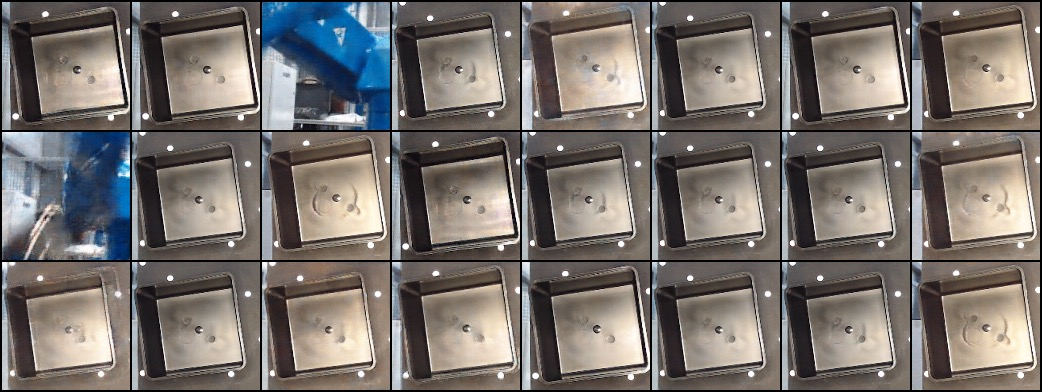
\includegraphics[width=\textwidth,height=\textheight,keepaspectratio]{../Chap4/Figures/SAGAN_fake_50000.jpg}
    \caption{Génération d'images à partir de la distribution modélisant l'espace latent du générateur d'un \textit{GAN}.}
    \label{fig:gan_sampling}
\end{figure}

La Figure \ref{fig:gan_sampling} montre des images générées à partir de tirages aléatoires dans l'espace latent du générateur d'un modèle \textit{SAGAN}.
On observe le meilleur réalisme des images obtenues, en comparaison des résultats donnés par un VAE \ref{fig:vae_sampling}.
La diversité des défauts est bien représentée. De plus, il est intéressant de remarquer que malgré le très faible nombre d'images représentant un bras robotique dans le jeu de données initial (1 erreur de capture pour 100 images), ces derniers sont représentés avec beaucoup de réalisme dans l'espace latent du générateur.
Un modèle GAN est peu robuste.
Il est sensible aux échantillons extrêmes d'un jeu de données.
Dans notre cas, cela peut être un avantage pour modéliser des défauts qui n'apparaissent pas souvent ; mais cela demande également une rigueur dans la construction du jeu de données, pour ne pas introduire d'images erronées, comme ici le bras robotique.

De même que pour le modèle \textit{VAE}, §\ref{subsubsec:vae}, la complexité de l'apprentissage d'un \textit{GAN} est très importante.
L'apprentissage du modèle est réalisé par descente de gradients stochastiques.
Les poids du modèle sont ajustés sur un sous-ensemble du jeu de données de taille $B$ échantillons (appelé mini-batch), pendant $T$ itérations.
La complexité de l'apprentissage est de l'ordre de $\bigO(T B^2 D + T B^2 d)$, avec $T$ le nombre d'itérations, $B$ le nombre d'échantillons dans un mini-batch, $D$ la dimension d'un échantillon et $d$ la dimension de l'espace latent.
Nous sommes limités par la capacité de mémoire de travail de notre processeur graphique à $B=64$ et $D=128^2$, d'où la complexité des calculs ($T=5000$, $B=64^2$, $D=128^2$). Nous obtenons une complexité de l'ordre de 350 Milliard d'opérations.
La durée de l'apprentissage de notre modèle GAN est de 10 heures sur un processeur graphique dédié (\textit{NVIDIA GTX 1080 Ti}).
Avec les ressources informatiques actuelles, seule une mise à jour hebdomadaire de ce modèle peut être envisagée.
Malgré le réalisme de la méthode, il est nécessaire de disposer d'importantes ressources de calculs pour mettre à jour le modèle à une fréquence journalière.

% TODO: BIGGAN \textit{BIGGAN} \cite{brock_large_2018}
% https://towardsdatascience.com/gan-ways-to-improve-gan-performance-acf37f9f59b
% https://medium.com/@jonathan_hui/gan-rsgan-ragan-a-new-generation-of-cost-function-84c5374d3c6e

% http://ganocracy.csail.mit.edu/tutorial/more_resources.html
% Lipschitz Generative Adversarial Nets https://arxiv.org/abs/1902.05687

% TODO:
% Modal loss instead of MSE !!!
% Late merging 4 VAE on 4 cameras, losses on each images reconstruction
% Compare UMAP reduction with VAE reduction

% Tesla ICML Multitask/Multiinstance learning. Which part of the model to train? Supsampling?

% Long Short Term Memory
% Jurgen Schmidhuber (1997).
% Discovering Neural Nets with Low Kolmogorov Complexity and High
% Generalization Capability.
% Neural Network
%
% Deep Belief Networks
% Geoff. Hinton and S. Osindero and Yeh Weh Teh (2006).
% A fast learning algorithm for deep belief nets.
% Neural Computation.

% Vapnik 2019: Rethinking statistical learning theory: learning using statistical invariants
% https://doi.org/10.1007/s10994-018-5742-0
% This paper introduces a new learning paradigm, called Learning Using Statistical Invariants (LUSI)
%page 39: 16 The idea of two-stage learning is also realized in deep neural networks (DNN), where, at the first stage (using “deep architecture”), an appropriate network is constructed and then, at the second stage, using standard for NN training procedures, the solution is obtained. DNN, however, cannot guarantee either that the constructed network contains a good approximation to the desired function or that it can find the best solution for the given network.
% Le choix des hyperparamètres est équivalent à l'introduction de prédicat.
% Il s'agit de trouver, de manière efficiente, le ou les quelques prédicats nécessaires et suffisants, à la construction du modèle optimal.

\section{Optimisation automatique des hyper-paramètres d'un modèle} \label{sec:auto_ml}
Les algorithmes présentés dans la section précédente possèdent plusieurs dizaines d'hyper-paramètres.
Leur ajustement est souvent crucial pour obtenir des performances satisfaisantes.
On parle d'optimisation des hyper-paramètres : on cherche à optimiser la performance du modèle pour la tâche à effectuer.
Il est également nécessaire de sélectionner les bonnes méthodes de préparation des données.
Le Tableau \ref{tab:cnn_hyperparameters} recense, par exemple, les hyper-paramètres des modèles à réseaux de neurones de convolutions profonds.
Des méthodes d'optimisation automatique de ces hyper-paramètres ont été proposées.
Cette optimisation est souvent appelée \textit{AutoML} (\textit{Automated Machine Learning}).
Dans le cas des réseaux de neurones profonds, l'architecture du réseau est également importante.
Elle doit être considérée comme de nombreux hyper-paramètres.
Le nombre de paramètres devient alors très grand et les algorithmes d'optimisation traditionnels deviennent limités ; la méta-descente de gradients et les algorithmes évolutionnistes deviennent plus adaptés §\ref{subsec:nas}.
Cette section propose de parcourir les méthodes les plus avancées et de discuter de leurs applications sur notre problématique de de contrôle de la conformité.

L'ensemble des expériences d'optimisation de modèles réalisées dans ces travaux ont utilisé la librairie \textit{Sacred} \cite{greff_sacred_2017}, afin de conserver un historique des hyper-paramètres et des performances associés.
Certaines de ces optimisations peuvent prendre plusieurs jours, c'est pourquoi il est nécessaire de sauvegarder l'évolution des performances pour éviter toute perte de ressources temporelles en cas d'erreur.
\textit{Sacred} permet également de rendre compte de la progression des optimisations et de surveiller toute erreur.

\subsection{Optimisation par recherche aléatoire} \label{subsec:random_search}
Afin de réaliser l'optimisation, il s'agit d'évaluer la performance de la méthode sur la plage de valeurs de chacun des hyper-paramètres.
Il est possible d'évaluer l'ensemble de la plage de valeurs de manière exhaustive, par une grille d'essais régulière, ce qui est coûteux sur le plan du calcul.
Une démarche plus économique est le tirage aléatoire sur la plage de valeurs, proposée par \citeauthor{bergstra_random_2012} \cite{bergstra_random_2012}.

\begin{figure}[hbtp]
    \centering
    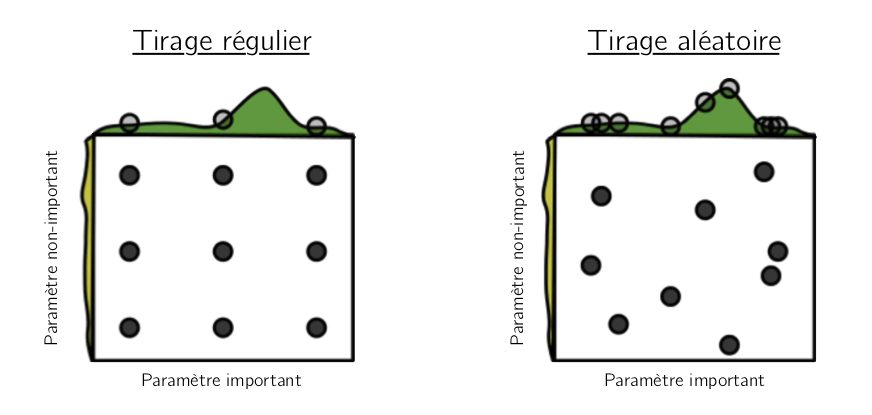
\includegraphics[width=0.80\textwidth,height=\textheight,keepaspectratio]{../Chap4/Figures/bergstra_RandomSearch2002.png}
    \caption{Optimisation d'une fonction à deux variables avec neuf essais. Figure reproduite de \cite{bergstra_random_2012}.}
    \label{fig:random_search}
\end{figure}

La Figure \ref{fig:random_search} présente un tirage de 9 essais pour trouver le maximum d'une fonction à deux dimensions.
Dans le cas de la recherche exhaustive, seuls trois essais permettent d'étudier la dimension horizontale.
Dans la recherche aléatoire, les 9 essais permettent d'étudier la dimension horizontale, ce qui est plus efficient.
Cette limite de la recherche exhaustive est d'autant plus importante que le nombre de dimensions étudiées est grand.
Des méthodes plus évoluées qui ont été proposées.

% https://slideslive.com/38917537/towards-semiautomated-machine-learning
% https://joaquinvanschoren.github.io/ML-course/slides_pdf/AutoML%20-%20Introduction.pdf

En 2011, \citeauthor{bergstra_algorithms_2011} \cite{bergstra_algorithms_2011} réalisent un état de l'art des méthodes d'optimisations d'hyper-paramètres, pour les modèles à réseaux de neurones profonds.
Ce travail montre l'intérêt de l'optimisation itérative, basée sur le critère de la prédiction de l'amélioration de performance du modèle (\textit{Expected Improvement}, proposée par \citeauthor{jones_taxonomy_2001} \cite{jones_taxonomy_2001}).
L'étude introduit deux méthodes d'optimisation.
Une méthode cherche à modéliser le problème d'optimisation par des processus stochastiques gaussiens et la seconde méthode \textit{TPE} propose une modélisation par noyaux, §\ref{subsubsec:tpe_opt}.
Ces méthodes s'appuient sur la construction de méta-modèles.
L'étude montre la supériorité de ces deux méthodes sur l'optimisation par tirage aléatoire.

\subsection{Optimisation par méta-modèle bayésien} \label{subsec:bayesian_opt}
% Start with a few (random) hyperparameter confgurations
% • Build a surrogate model to predict how well other confgurations will work: mean and standard deviation (blue band)
% • Any probabilistic regression model: e.g. Gaussian processes
% • To avoid a greedy search, use an acquisition function to trade off
% exploration and exploitation, e.g. Expected Improvement (EI)
% • Sample for the best confguration under that function μ σ H
%
% Repeat
% • Stopping criterion:
% • Fixed budget (time, evaluations)
% • Min. distance between confgs
% • Threshold for acquisition function
% • Still overfts easily
% • Convergence results
% • Good for non-convex, noisy objectives
% • Used in AlphaGo
% 
% Gaussian processes
% + uncertainty, extrapolation
% - Scalability (cubic)
% Sparse GPs[Lawrence et al. 2003]
% Random embeddings [Wang et al. 2013]
% - Robustness? Meta-BayesOpt to optimize kernel [Malkomes et al. 2016]
% Neural networks + Bayesian LR [Snoek et al. 2015]
% + Scalable, Learns basis expansion
% Bayesian neural networks [Springenberg et al. 2016]
% + Bayesian - Scalability not studied yet

Cette démarche cherche dans un premier temps à modéliser le lien entre les hyper-paramètres $\boldsymbol{x}$ et les performances $y = f(\boldsymbol{x}, \boldsymbol{D})$ du modèle $f$ appris sur le jeu de données $\boldsymbol{D}$.
Il s'agit ensuite de résoudre le problème d'optimisation des hyper-paramètres $\boldsymbol{x}$ dans l'espace de valeurs des hyper-paramètres $\mathcal{X}$, afin de trouver les hyper-paramètres optimaux $\boldsymbol{x}_{\star}$.
L'Équation \ref{eq:hp_optimization} présente ce problème dans le cas où la sortie de $f$ est l'erreur d'apprentissage du modèle.

\begin{equation} \label{eq:hp_optimization}
\boldsymbol{x}_{\star} \in \underset{\boldsymbol{x} \in \mathcal{X}}{\arg \min } f(\boldsymbol{x})
\end{equation}

$f$ est approximée par un méta-modèle $\mathcal{M}$, sous la forme de procédés gaussiens\footnote{La théorie des procédés gaussiens a été développée par \citeauthor{matheron_principles_1963} \cite{matheron_principles_1963}. Cette démarche est aussi appelée \textit{krigeage}, d'après les travaux originaux de \citeauthor{krige_statistical_1951} \cite{krige_statistical_1951}.}, qui permet de prendre en compte l'incertitude sur les futures évaluations de $m$, Équation \ref{eq:hp_gp}.
\begin{equation} \label{eq:hp_gp}
y = f(\boldsymbol{x}) \sim \mathcal{M}\left(\mu(\boldsymbol{x}), k\left(\boldsymbol{x}, \boldsymbol{x}^{\prime}\right)\right)
\end{equation}

On cherche à modéliser la distribution de probabilité de $y$ connaissant les hyper-paramètres $\boldsymbol{x}$ : $p(y | \boldsymbol{x})$.
Le procédé gaussien $\mathcal{M}$ est défini par sa moyenne $\mu$ et son noyau $k$ (différents noyaux sont présentés dans la Section précédente §\ref{eq:kernels}).
Le coût de l'optimisation des procédés gaussiens est néanmoins de l'ordre de $\bigO(N^3)$.
L'optimisation de $f$ nécessite généralement de 10 à 100 évaluations de la fonction.
Chaque évaluation de la fonction possède le coût de l'apprentissage du modèle sur le jeu de données complet.
Ce coût est très grand et il est nécessaire de limiter au maximum le nombre d'évaluations du méta-modèle $\mathcal{M}$.
Des modèles différents des coûteux procédés gaussiens ont été proposés.
Nous les présentons dans les Sections suivantes §\ref{subsubsec:rf_opt}, §\ref{subsubsec:tpe_opt}.

Il est également nécessaire de choisir judicieusement les points d'évaluations $\boldsymbol{x}_{n+1}$ de $f$ à la prochaine évaluation.
Il n'est pas judicieux de choisir $\boldsymbol{x}_{n+1} = \mu{x_{n}}$ dans le cas où des minima locaux existeraient.
Le dilemme de l'optimisation itérative apparait : c'est le choix entre l'\textit{exploration} de $f$ pour construire un modèle $\mathcal{M}$ pertinent qui représente tous les minimas (dont le minimum de $f$), et l'\textit{exploitation} des valeurs de $y = f(\boldsymbol{x}_{n+1})$ qui permet d'atteindre le minimum $y_{\star}$ et trouver $\boldsymbol{x}^{\star}$.
Dans le cas de l'optimisation bayésienne, l'\textit{exploration} cherche à choisir un point qui diminuera les régions où l'incertitude du modèle est grande.
C'est pourquoi \citeauthor{jones_efficient_1998} \cite{jones_efficient_1998} proposent le critère de la prédiction de l'amélioration de performance prédite (\textit{Expected Improvement}), Équation \ref{eq:ei}.

\begin{equation} \label{eq:ei}
{EI}_{p(f | D)}\left[\max \left(y_{\star}-f(\boldsymbol{x}), 0\right)\right]
\end{equation}

Lors de la prochaine évaluation de $f$, les valeurs $\boldsymbol{x}_{n+1}$ seront choisies pour maximiser ce critère.
Cela permet de choisir les valeurs des hyper-paramètres optimales pour l'évaluation suivante de $f$.
D'autres critères, que nous ne pouvons détailler ici, existent.
Ils sont étudiés en réponse aux problèmes de bandits à N bras.
%https://www.cse.wustl.edu/~garnett/cse515t/spring_2015/files/lecture_notes/12.pdf

% SOTA+Monte Carlo: Wilson, James, Frank Hutter, and Marc Deisenroth. “Maximizing acquisition functions for Bayesian optimization.” In Advances in Neural Information Processing Systems, pp. 9906–9917. 2018.

\subsubsection{Forêts d'Arbres décisionnels} \label{subsubsec:rf_opt}
% Random Forests [Hutter et al. 2011, Feurer et al. 2015]
La méthode \textit{SMAC} (\textit{Sequential Model-Based Algorithm Configuration}) est proposée par \citeauthor{hutter_sequential_2011} \cite{hutter_sequential_2011}.
La démarche est identique à la modélisation gaussienne, mais elle utilise ici des Forêts d'Arbres décisionnels (§\ref{parag:random_forests}).
La sélection des premiers essais à réaliser peut être effectuée à partir des plans d'expériences, §\ref{subsec:doe}.
Un plan hypercube latin ou une séquence de \citeauthor{sobol_distribution_1967} §\ref{parag:doe_lhs} est généralement utilisé.
% F. Hutter. Automated Configuration of Algorithms for Solving Hard Computational Problems. PhD thesis, University of British Columbia, 2009.
% SMAC3:sequential model-based algorithm configuration
% - Factorial
% - Latin Hypercube
% - Sobol
% Frequentist uncertainty estimate (variance)
% + scalable, complex HPs - uncertainty, extrapolation
% Φz P BLR surrogate φz(λ)i (λi,P

% Random Forests (SMAC) example:
La librairie \textit{auto-sklearn} \cite{feurer_efficient_2015} utilise également les Forêts d'arbres décisionnels.
% https://www.kdnuggets.com/2016/10/interview-auto-sklearn-automated-data-science-machine-learning-team.html
% Combined Algorithm Selection and Hyperparameter optimization (CASH):
Cette librairie utilise la majorité des algorithmes de la librairie \textit{Scikit-Learn} \cite{pedregosa_scikit-learn_2011}, afin de construire automatiquement le modèle optimal.
Cela représente la possibilité d'utiliser 15 classifieurs et 14 méthodes de prétraitement des données, ce qui introduit un nombre conséquent de 110 hyper-paramètres.
Cet algorithme utilise un méta-modèle préalablement appris sur un grand nombre de jeux de données, afin de sélectionner les valeurs des hyper-paramètres initiaux.
Cette démarche a été proposée par \citeauthor{feurer_initializing_2015} \cite{feurer_initializing_2015}.
À la manière d'un expert humain qui a appris à prioriser certains algorithmes en fonction du jeu de données auquel il fait face, un méta-modèle est construit sur 140 jeux de données.
Ce méta-modèle permet de sélectionner les hyper-paramètres initiaux en fonction du jeu de données en présence.
Ce travail montre la pertinence du méta-modèle pour la sélection des essais initiaux, en comparaison d'une sélection basée, par exemple, sur un plan latin hypercube §\ref{parag:doe_lhs}.
Enfin, \textit{auto-sklearn} propose de construire un modèle qui agrège plusieurs méthodes différentes en fonction de leurs performances, dans une démarche ensembliste §\ref{parag:bagging}.

La Figure \ref{fig:autosk_result} montre le résultat de l'exploration des multiples classifieurs par \textit{auto-sklearn}.
Le classifieur le plus performant est ici le \textit{Stochastic Gradient Boosting} §\ref{parag:boosting}, à contrario d'une durée d'apprentissage importante.

\begin{figure}[hbtp]
    \centering
    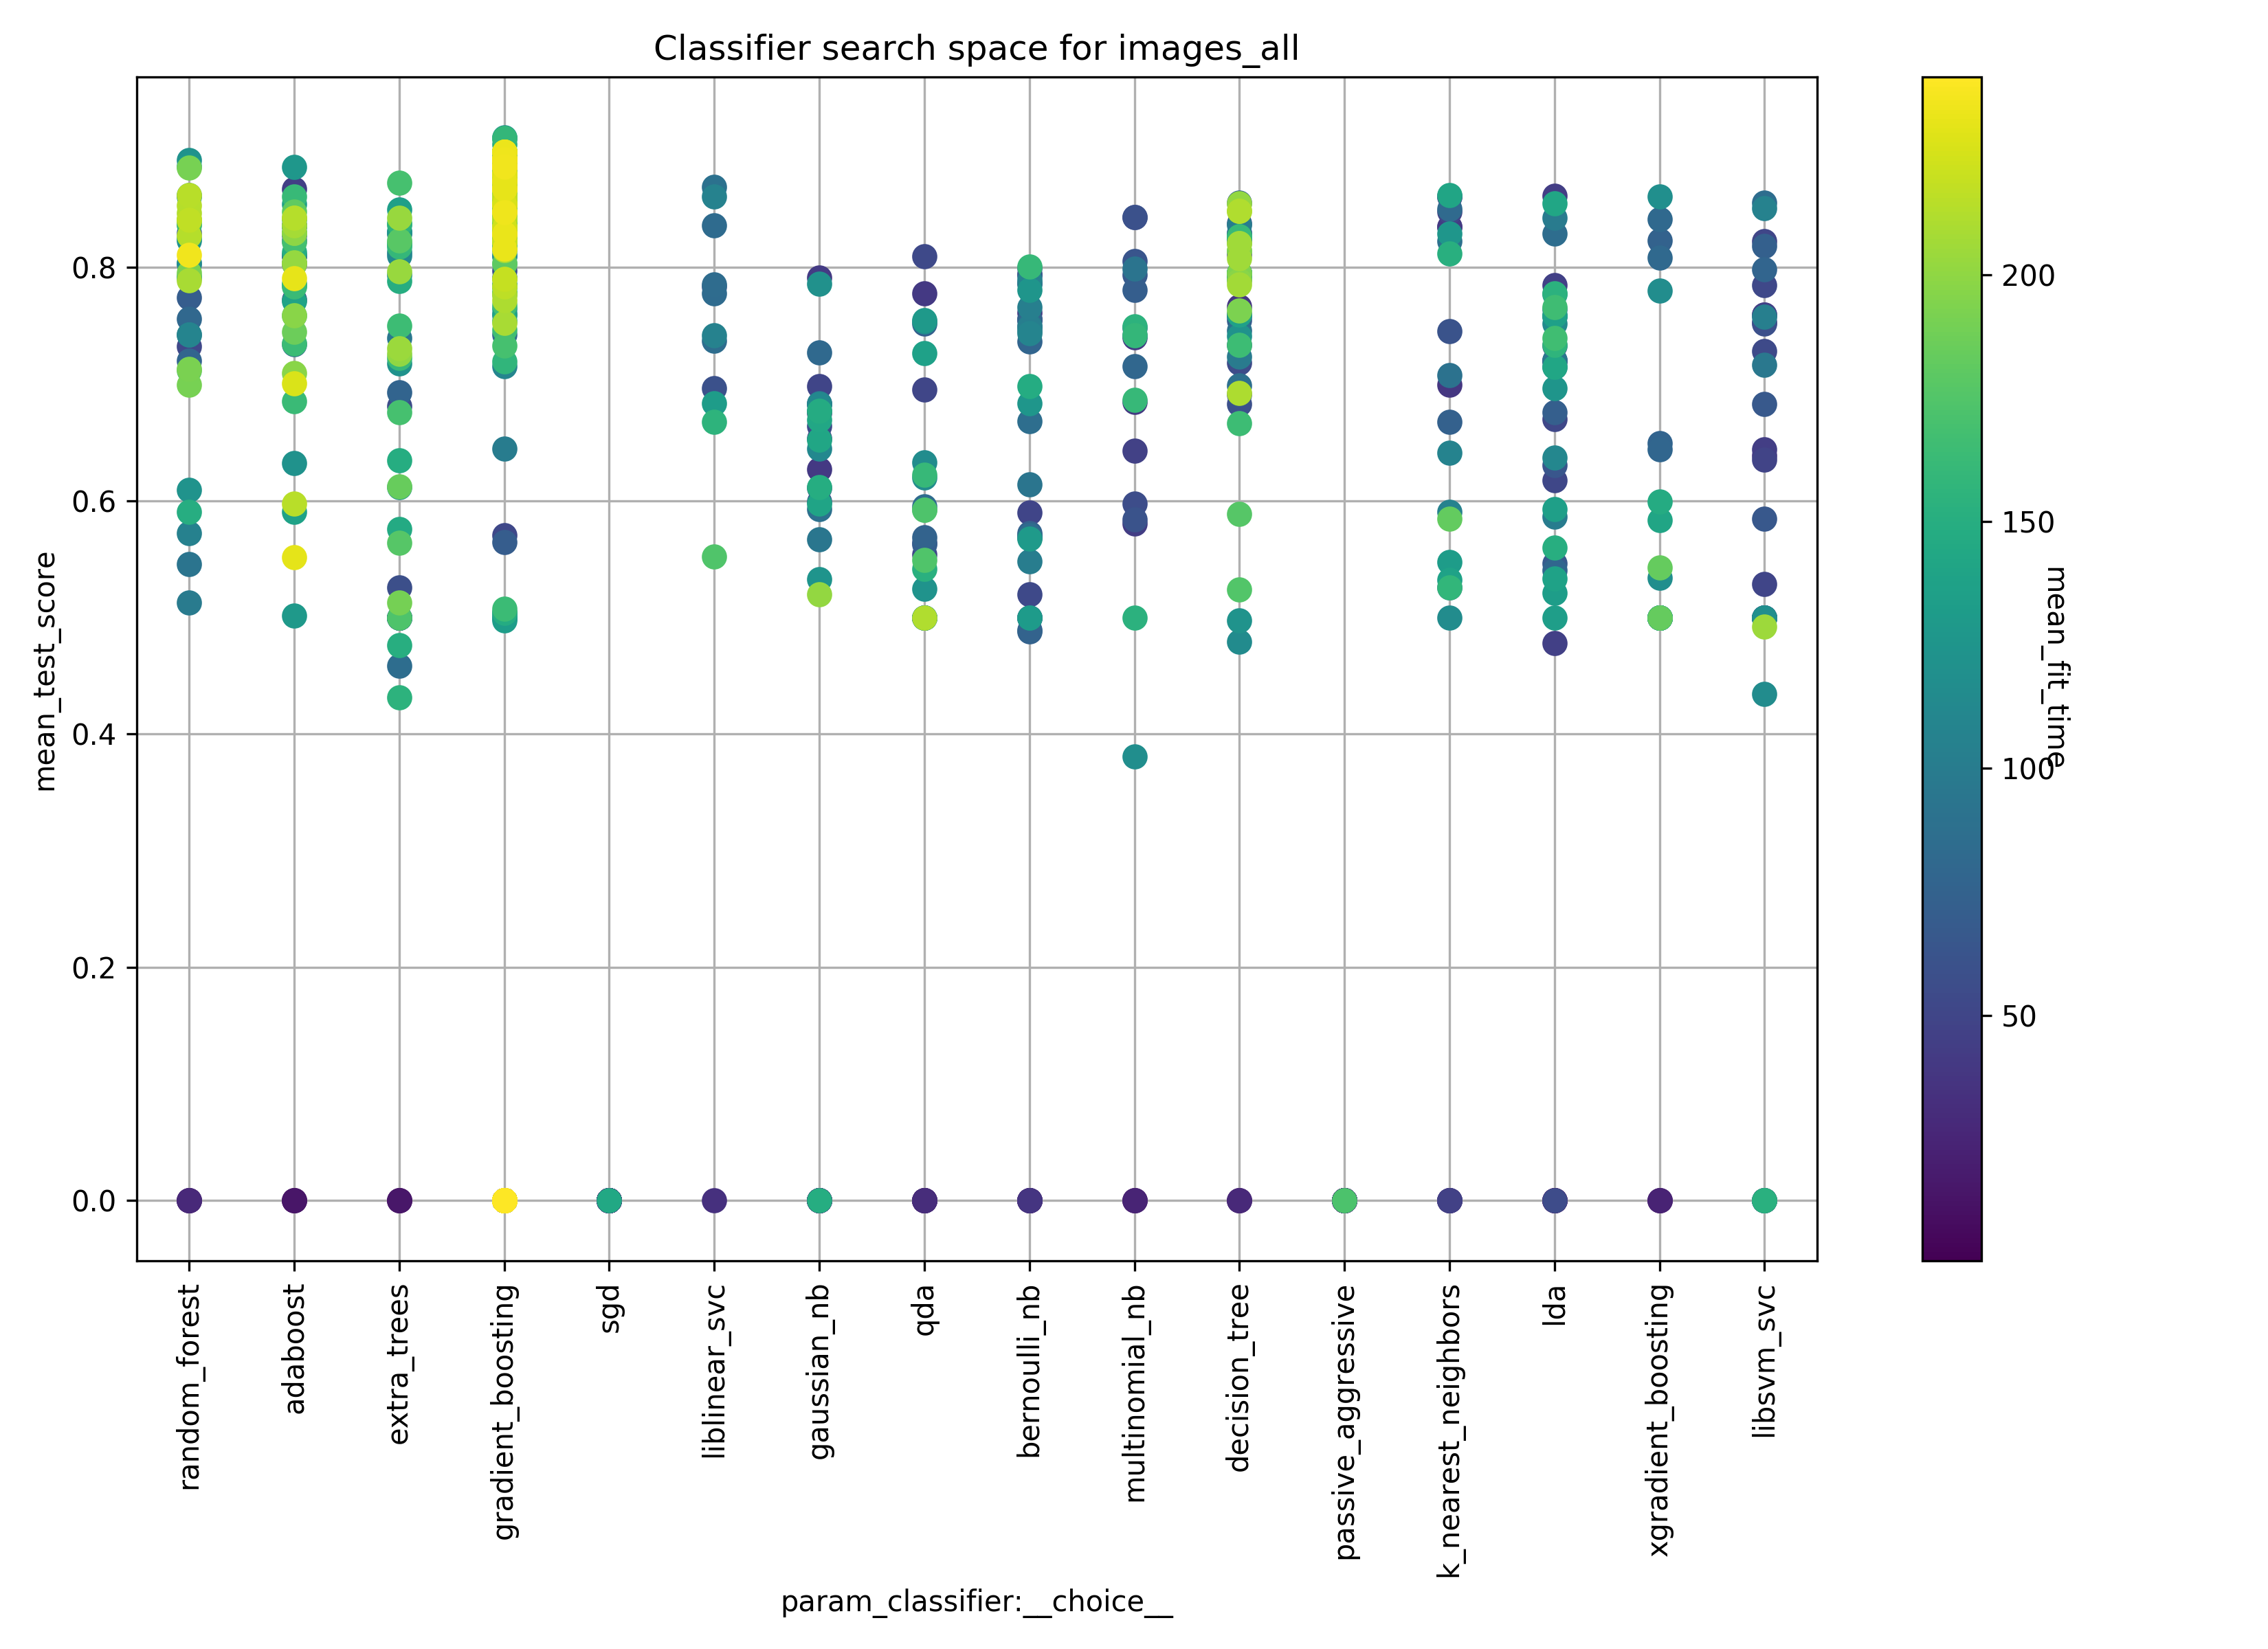
\includegraphics[width=\textwidth,height=\textheight,keepaspectratio]{../Chap4/Figures/cv_results_images_all.png}
    \caption{Optimisation d'un modèle appris de manière supervisée, à l'aide de la librairie \textit{auto-sklearn} \cite{feurer_efficient_2015}.}
    \label{fig:autosk_result}
\end{figure}


\subsubsection{Estimateur par noyaux structuré en arbre} \label{subsubsec:tpe_opt}
La libraire \textit{hyperopt} \cite{bergstra_making_2013} (\textit{HYPER-parameter OPTimization}) implémente la recherche aléatoire §\ref{subsec:random_search} et l'algorithme \textit{TPE} (\textit{Tree-structured Parzen Estimator}) \cite{bergstra_algorithms_2011} qui réalise une approximation de la fonction $f$ par estimation par noyau \footnote{L'estimation par noyau (\textit{kernel density estimator}) est aussi appelée méthode de Parzen-Rosenblatt, car elle a été initiée par Rosenblatt en 1956 et développée par Parzen en 1962.}.
% Parzen E. (1962). On estimation of a probability density function and mode, Ann. Math. Stat. 33, pp. 1065-1076
% http://jaberg.github.io/hyperopt/
% https://optunity.readthedocs.io/en/latest/index.html
% Cette méthode est parallélisable et produit des résultats équivalents que au critère \textit{Expected Improvements}.
% 1.Test some hyperparameters
% 2. Separate into good and bad hyperparameters (with some quantile)
% 3. Fit non-parametric KDE for and
% 4. For a few samples, evaluate
% Shown to be equivalent to EI!
% Efficient, parallelizable, robust, but less sample efficient than GPs
La modélisation de chaque hyper-paramètre est structurée dans un arbre de recherche.
Le parcours de l'arbre permet de réaliser l'optimisation entre de multiples paramètres.
Une limite forte de cette méthode est que les interactions entre chaque hyper-paramètres ne sont pas prises en compte dans le modèle car chaque hyper-paramètres disposent de leur branche indépendante sur l'arbre.
Dans le cas où deux hyper-paramètres sont inter-dépendants, cette méthode est moins performante que les procédés gaussiens §\ref{subsec:bayesian_opt}.

Dans le cas de l'optimisation bayésienne, on cherche à modéliser la distribution de probabilité de $y$ connaissant les hyper-paramètres $\boldsymbol{x}$ : $p(y | \boldsymbol{x})$.
Dans le cas de l'estimation par densité de noyaux, on cherche à modéliser la distribution de probabilité de $p(\boldsymbol{x} | y)$ et la distribution $p(y)$.
Le théorème de Bayes permet d'obtenir $p(\boldsymbol{x} | y) = p(y) p(y | \boldsymbol{x})$.
À chaque évaluation de $f$, on sépare les combinaisons d'hyper-paramètres qui obtiennent les meilleurs scores $y \le y*$ pour $\boldsymbol{x}^{top}$ et on définit la distribution $m(\boldsymbol{x})=p(\boldsymbol{x}^{meilleurs} | y)$.
Les combinaisons, dont le score est inférieur à $y*$, définissent la distribution $b(\boldsymbol{x})=p(\boldsymbol{x}^{bof} | y)$.
On choisit généralement la limite $y*$ comme le premier quartile, tel que $p(y < y*) = 0.75$.
\cite{bergstra_algorithms_2011} montre que le rapport $m/b$ est équivalent au critère de la prédiction de l'amélioration de performance (§\ref{subsec:bayesian_opt}), ce qui permet de choisir les prochains essais en minimisant $m/b$.

% Dernièrement, la librairie \texitt{HyperOpt-sklearn} [Komer et al. 2019]

\subsection{Méthodes de réduction du coût d'évaluation du méta-modèle} \label{subsec:reduce_opt}
L'évaluation de $f(\boldsymbol{x}, \boldsymbol{D})$ nécessite l'apprentissage d'un modèle sur le jeu de données $\boldsymbol{D}$, ce qui peut prendre plusieurs heures dans le cas de l'utilisation de réseaux de neurones profonds (\textit{Deep Learning} \ref{subsubsec:deep_learning}).
C'est pourquoi des démarches ont récemment été proposées.
% I We often have access to cheap-to-evaluate approximations ˜f(·, b) of the true objective functionf(·), so called fidelities.

\subsubsection{Évaluations partielles des configurations dans une durée limitée} \label{subsubsec:successive_halving}
Dans le cadre des algorithmes bandits, \citeauthor{jamieson_nonstochastic_2015} \cite{jamieson_nonstochastic_2015} propose la méthode \textit{Successive Halving} qui permet de réduire le coût de l'optimisation de $f$.
Il s'agit d'évaluer uniquement les configurations d'hyper-paramètres qui présentent un apprentissage de $f$ rapide.
Dans cet objectif, plusieurs évaluations de $f$ sont lancées en parallèle.
Une durée maximale $b$ pour les évaluations est définie.
À la fin de cette durée $b$, l'erreur d'apprentissage de chaque $f$ est évaluée.
La moitié des modèles qui possèdent les erreurs les plus petites est conservée.
La durée maximale $b$ est alors incrémentée et l'évaluation des modèles restants est à nouveau lancée.
Cette démarche est équivalente à l'évaluation itérative de la dérivée de l'erreur d'apprentissage des modèles, tout en étant massivement parallélisable.

Cette méthode s'appuie sur l'hypothèse que le meilleur modèle $f$ aura une vitesse d'apprentissage plus rapide que les autres.
% Régulièrement, au sens des itérations de l'apprentissage, la moitié des modèles qui possèdent les dérivées les plus petites sont arrêtés.
La limite de cette méthode est qu'il y a un risque de ne pas explorer des configurations d'hyper-paramètres qui donneraient de meilleures performances, mais qui sont plus lentes que de mauvaises configurations.
C'est une hypothèse forte qui a été vérifiée dans ce travail sur des bases de données d'apprentissages conséquentes.

\begin{figure}[tbp]
    \centering
    \begin{subfigure}{.475\textwidth}
        \centering
        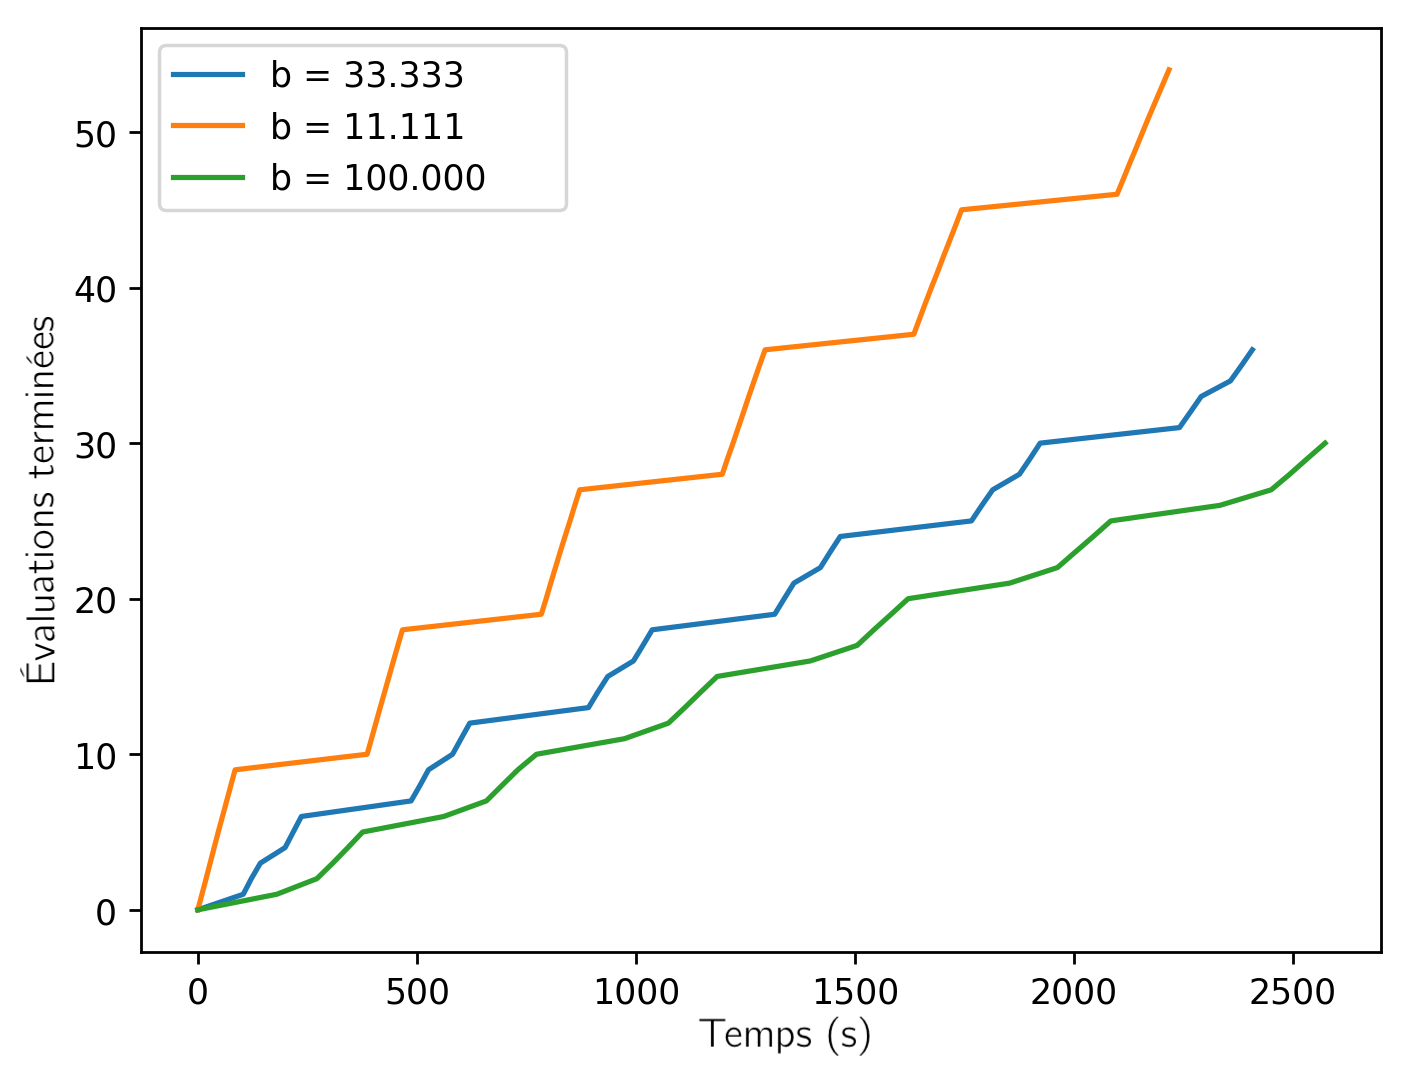
\includegraphics[width=\linewidth]{HPS_finished_runs_over_time_images_all.png}
        \caption{Nombre d'évaluations de $f$ réalisées en fonction de la limite de temps $b$.}
        \label{fig:succesive_halving_time}
    \end{subfigure}\hfill% or \hspace{5mm} or \hspace{0.3\textwidth}
    \begin{subfigure}{.485\textwidth}
        \centering
        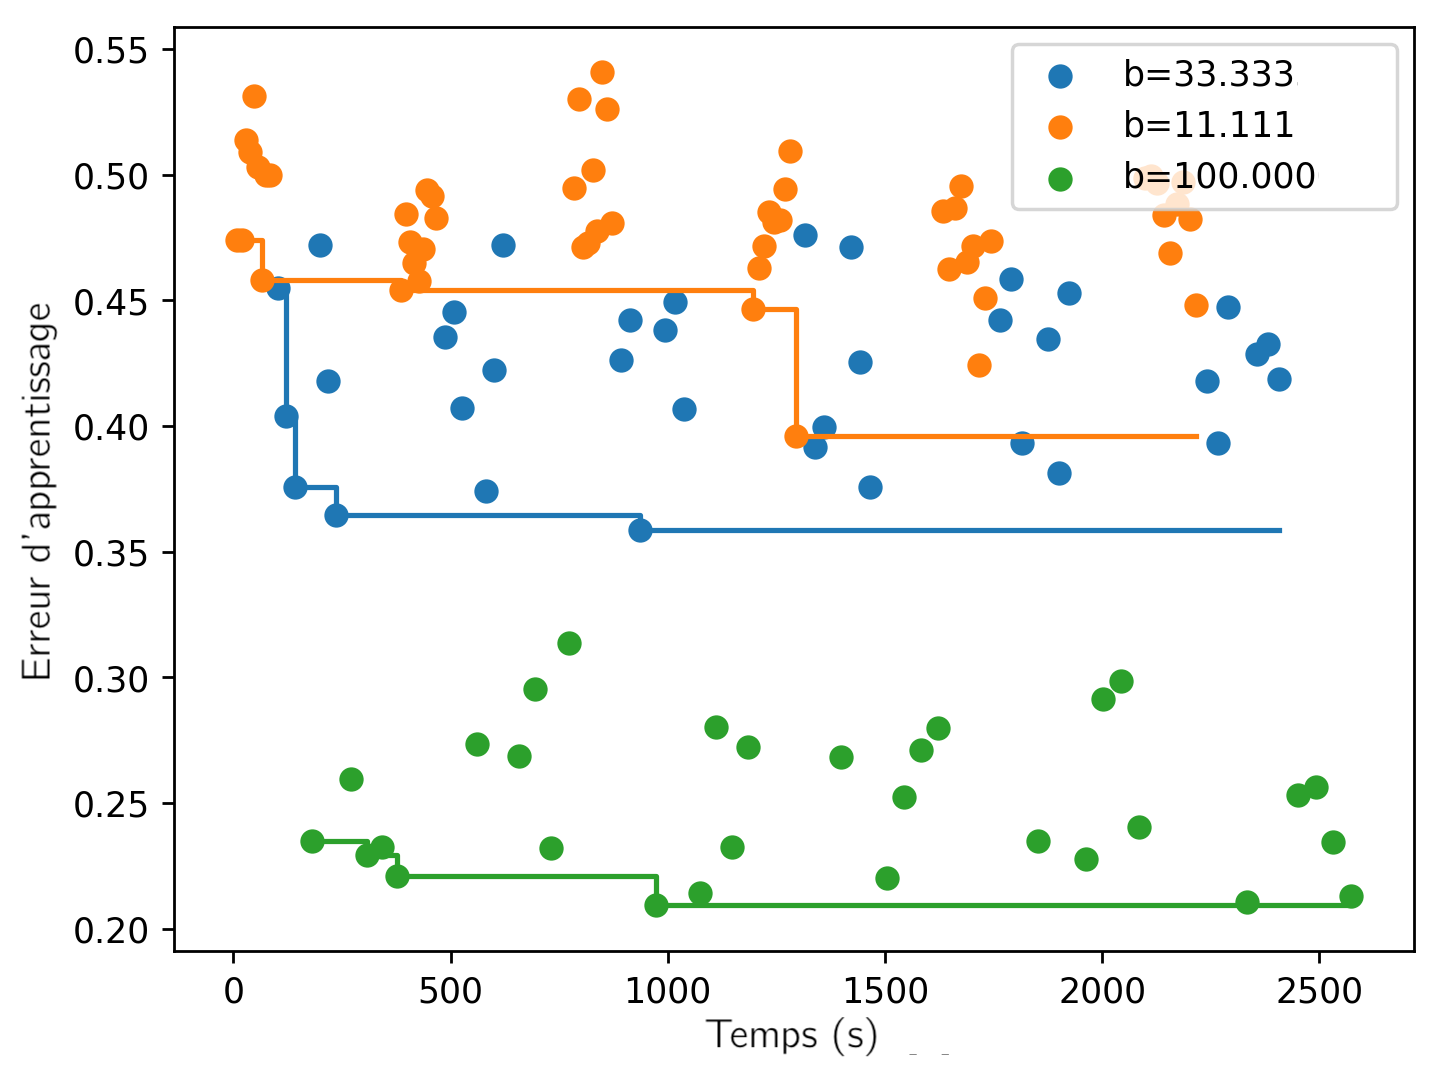
\includegraphics[width=\linewidth]{HPS_losses_over_time_images_all.png}
        \caption{Erreur lors de l'apprentissage de $f$ en fonction de la limite de temps $b$.}
        \label{fig:succesive_halving_loss}
    \end{subfigure}
    \caption{Évaluation partielle de $f$ en fonction de $b$.}
    \label{fig:succesive_halving}
\end{figure}

La Figure \ref{fig:succesive_halving_time} présente l'évolution du nombre d'évaluations de $f$ en fonction de $b$.
L'augmentation de $b$ limite le nombre d'évaluations de $f$ réalisées.
Il est nécessaire de sélectionner les bonnes configurations d'hyper-paramètres, ce que fait le méta-modèle.
La Figure \ref{fig:succesive_halving_loss} présente l'erreur d'apprentissage de modèles $f$, obtenue pour différentes valeurs de $b$.
L'augmentation de $b$ permet d'augmenter les performances du modèle.
% Often in practice, promising configurations tend to score higher, relatively to the worst ones, even early on in the process.
% There we go! This is what SuccessiveHalving is all about! Here is how the algorithm, makes use of this assumption:
% Randomly sample a set of hyperparameter configurations
% Evaluate the performances of all currently remaining configurations
% Throw out, the bottom half of the worst scoring configurations
% Go back to 2. and repeat until one configuration remains.
% Instead of wasting a lot of training time in configurations that will lead us nowhere, SuccessiveHalving throws as soon as possible. Hence, more training time, i.e. resources, can be allocated to more potentially valuable models.
%
% A huge question when applying SuccessiveHalving, is finding the right trade-off between total ressources and total number of configurations.
% Smaller learning rates often go hand in hand with more resources, more trees in case of (extreme) gradient boosting or more epochs for neural networks.
% How can we tune such a choice? HyperBand proposes a solution, but this one is for next time!

L'utilisation de l'arrêt prématuré §\ref{parag:early_stopping} pendant l'apprentissage de chaque modèle $f$ est également proposée par \citeauthor{domhan_speeding_2015} \cite{domhan_speeding_2015}.
Ce travail introduit l'utilisation d'un modèle prédictif de l'évolution de l'erreur d'apprentissage.
Pour cela, pendant l'apprentissage de $f$, un modèle bayésien (méthode Monte-Carlo par chaînes de Markov) est construit pour prédire l'évolution future de l'erreur d'apprentissage.
Si l'évolution est défavorable, l'apprentissage est stoppé avant la fin du nombre d'itérations prédéfinies.
Dans le cas d'une utilisation de cette méthode pour l'optimisation des hyper-paramètres de réseaux de neurones profonds, les auteurs évaluent le gain à un facteur deux.

\subsubsection{Évaluation de $f$ sur un sous-ensemble des données} \label{subsec:subsampling}
\citeauthor{klein_fast_2016} \cite{klein_fast_2016} propose d'évaluer $f$ sur une partition réduite du jeu de données, (cette méthode est prénommée \textit{Fabolas}).
La dimension du sous-ensemble du jeu de données est progressivement augmentée au fur et à mesure que des configurations d'hyper-paramètres satisfaisantes sont trouvées.
La vitesse de l'optimisation est augmentée d'un facteur 10 en comparaison d'une optimisation bayésienne ou de la méthode \textit{Hyperband} §\ref{subsec:bandit}.
Associée à l'évaluation partielle par arrêt prématuré, cette méthode est très efficace pour limiter le coût de l'évaluation.

\subsection{Optimisation par algorithmes bandits} \label{subsec:bandit}
% https://medium.com/criteo-labs/hyper-parameter-optimization-algorithms-2fe447525903
% https://maelfabien.github.io/machinelearning/HyperOpt/
Les méthodes bandits à N bras consistent en l'évaluation massivement parallèle de multiples modèles, et en la sélection des meilleurs, à chaque itération.
La méthode \textit{Hyperband} est proposée par \citeauthor{li_hyperband_2016} \cite{li_hyperband_2016}.
Elle utilise la démarche d'arrêt prématuré de l'apprentissage §\ref{subsubsec:successive_halving}.
% https://openreview.net/forum?id=ry18Ww5ee
L'étude des auteurs démontre que, dans le cas où l'espace des hyper-paramètres est organisé de la pire des façons pour l'algorithme, la recherche d'une solution optimale amènera à un coût d'optimisation 5 fois plus grand qu'avec une recherche aléatoire §\ref{subsec:random_search}.
À contrarior, dans le cas où l'espace des hyper-paramètres est organisé dans le meilleur cas, la méthode à un coût 10 fois moins grand qu'une recherche aléatoire.
La méthode utilise également l'apprentissage progressif sur des sous-ensembles des données §\ref{subsec:subsampling}.
Les auteurs concluent sur la possibilité d'utiliser les plans d'expériences §\ref{subsec:doe} pour sélectionner les configurations d'hyper-paramètres à évaluer en premier.
% from BOHB:
% Hyperband balances very aggressive evaluations with many configurations on the smallest budget and very conservative runs on the full budget. This helps it guard against having trusted cheap budgets too much.
%
% In practice HB performs very well for small to medium budgets and typically outperforms random search and vanilla BO quite easily in that setting. However, its convergence is limited by its reliance on randomly-drawn configurations: with larger budgets its advantage over random search diminishes. An example of this is given in the plot below.
%

Récemment, la méthode \textit{BOHB} (\textit{Bayesian Optimization and HyperBand}) a été proposée par \citeauthor{falkner_combining_2017} \cite{falkner_combining_2017, falkner_bohb_2018}.
% http://ais.informatik.uni-freiburg.de/teaching/ws18/deep_learning_lab/presentation_automl.pdf
% Combining Hyperband with Bayesian Optimization [Falkner et al., 2017]
% https://www.automl.org/blog_bohb/
Elle associe les techniques d'\textit{Hyperband} pour la sélection du nombre de configurations à évaluer dans un temps limité, et ajoute l'optimisation d'un méta-modèle bayésien (similaire aux noyaux structurés en arbre \textit{TPE} §\ref{subsubsec:tpe_opt}) pour sélectionner les meilleures configurations à évaluer.
À la différence de \textit{Hyperband} qui sélectionne les configurations de manière aléatoire, le méta-modèle permet de prendre en compte l'information sur les configurations acquise au fur et à mesure des évaluations.
La sélection des configurations à évaluer est plus pertinente, ce qui permet d'atteindre la configuration optimale avec environ deux fois moins d'évaluations que \textit{Hyperband}.
% Hyperband:
% - very efficient in terms of anytime performance
% - due to the random sampling, cannot reuse previously gain knowledge and take a long time to converge
% Bayesian optimization:
% - in its standard form it cannot exploit fidelites (however, several extensions exist)
% - in the most cases converges faster than random search
% Can we combine both methods?
% Bayesian optimization is an efficient strategy for hyperparameter optimization
% BOHB combines Hyperband with Bayesian optimization to combine the strengths of both methods
%
% BOHB combines Bayesian optimization (BO) and Hyperband (HB) to combine both advantages into one, where the Bayesian optimization part is handled by a variant of the Tree Parzen Estimator (TPE; Bergstra et al., 2011) with a product kernel (which is quite different from a product of univariate distributions).  BOHB relies on HB to determine how many configurations to evaluate with which budget, but it replaces the random selection of configurations at the beginning of each HB iteration by a model-based search, where the model is trained on the configurations that were evaluated so far.
%
% BOHB’s strong anytime performance (desideratum 1) stems from its use of Hyperband. Quickly evaluating lots of configurations on small budgets allows BOHB to quickly find some configurations that are promising. The strong final performance (desideratum 2) stems from BOHB’s BO part as the guided search in the end is able to refine the selected configurations.
% 
% The plot at the top of the section shows that BOHB behaves like Hyperband in the beginning and later profits from the constructed BO model. In the beginning, both BOHB and Hyperband show a 20x speedup over  Random Search and standard BO. With increasing budgets, Hyperband’s improvement over Random Search diminishes but BOHB still continues to improve, with a speedup of 55x over Random Search.
% 
% BOAH: A Tool Suite for Multi-Fidelity Bayesian Optimization & Analysis of Hyperparameters
% implements BOHB and analysis
% 
% Monte-Carlo Tree Search
% Pipeline search: Monte Carlo Tree Search
% • Use MCTS to search for optimal pipelines
% • Optimize the structure and hyperparameters simultaneously by building a surrogate model to predict confguration performance
% • Bayesian surrogate model: MOSAIC [Rakotoarison et al. 2019]

Afin d'observer l'influence des différents hyper-paramètres sur la performance du modèle, nous réalisons une analyse de la variance des hyper-paramètres pour $f$ (\textit{ANAVAR}/\textit{ANOVA}), en utilisant la librairie \citeauthor{hutter_efficient_2014} \cite{hutter_efficient_2014}.
Lorsque le nombre d'évaluations du modèle est assez grand ($> 100$), cela permet de rendre compte des interactions possibles entre les hyper-paramètres.
La Figure \ref{fig:fanova} présente les résultats pour deux couples d'hyper-paramètres (\textit{beta} est ici un terme de pénalisation des poids §\ref{parag:weights_decay}).
On observe que les surfaces de réponses sont complexes.
De plus, le nombre d'hyper-paramètres présent est ici de 38 et des interactions existent entre les hyper-paramètres.
C'est pourquoi un expert humain aurait eu de grandes difficultés à réaliser cette optimisation manuellement, dans un espace continu de dimensions 38.

\begin{figure}[tbp]
    \centering
    \begin{subfigure}{.49\textwidth}
        \centering
        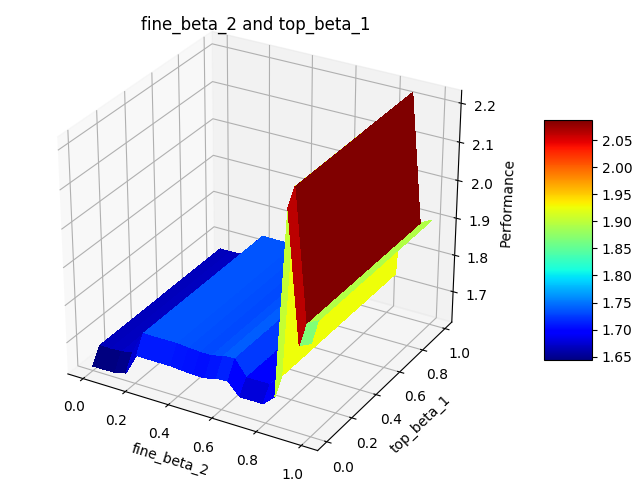
\includegraphics[width=\linewidth]{fine_beta_2_top_beta_1.png}
        \label{fig:fanova_a}
    \end{subfigure}\hfill% or \hspace{5mm} or \hspace{0.3\textwidth}
    \begin{subfigure}{.49\textwidth}
        \centering
        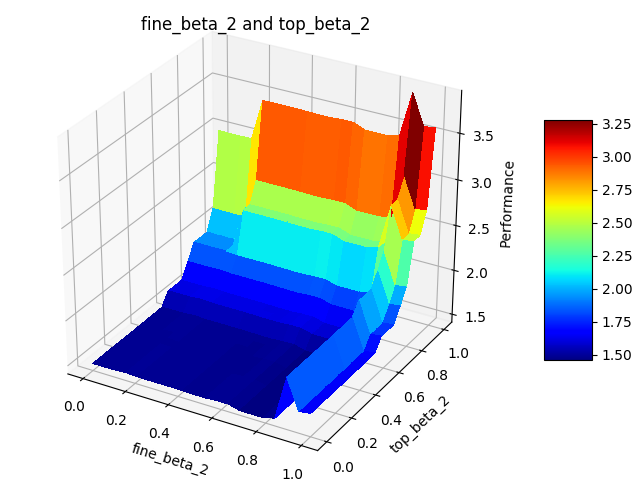
\includegraphics[width=\linewidth]{fine_beta_2_top_beta_2.png}
        \label{fig:fanova_b}
    \end{subfigure}
    \caption{\textit{fANOVA} des hyper-paramètres suite à l'optimisation avec \textit{BOHB}.}
    \label{fig:fanova}
\end{figure}

\subsection{Optimisation par algorithmes évolutionnistes} \label{subsec:evolution}
% http://automl.info/tpot/
Proposée en 2016 dans \citeauthor{olson_evaluation_2016, olson_automating_2016} \cite{olson_evaluation_2016, olson_automating_2016}, \textit{TPOT} (\textit{Tree-Based Pipeline Optimization Tool}) s'appuie sur un algorithme génétique pour explorer les configurations d'hyper-paramètres et sur une Forêt d'Arbres décisionnels §\ref{parag:random_forests} pour optimiser le meilleur modèle.
% https://rstudio-pubs-static.s3.amazonaws.com/423824_f67e5db15f6e4e59bcf284208e441cfd.html
% Tree-based pipeline optimization
% • Start with random pipelines, best of every generation will cross-over or mutate
% • GP primitives include data copy and feature joins: trees
% • Multi-objective optimization: accurate but short
% • Easy to parallelize
% • Asynchronous evolution (GAMA)
% copy, change, insert, shrink

Nous avons appliqué cette méthode dans \citetitle{nagorny_polarimetric_2019} \cite{nagorny_polarimetric_2019}, sur notre problématique de l'apprentissage supervisé d'un modèle pour le contrôle de la conformité.
Sur des images de dimensions $331 \times 331$ pixels, l'évaluation de 300 modèles $f$ est effectuée en 14 heures.
Le gain de performances suite à l'optimisation des hyper-paramètres est de 2\%.
L'algorithme a trouvé le meilleur modèle possible en une demi-journée.
Un expert humain n'aurait certainement pas réussi à trouver le meilleur modèle en si peu de temps.
Malgré la durée qui est importante, \textit{TPOT} permet de remplacer plusieurs journées d'expertise d'un ingénieur en sciences des données.

%% Dernièrement, l'algorithme GAMA: Gijsbers, Vanschoren 2019
%
% https://deepmind.com/blog/article/population-based-training-neural-networks
% PBT - like random search - starts by training many neural networks in parallel with random hyperparameters. But instead of the networks training independently, it uses information from the rest of the population to refine the hyperparameters and direct computational resources to models which show promise. This takes its inspiration from genetic algorithms where each member of the population, known as a worker, can exploit information from the remainder of the population. For example, a worker might copy the model parameters from a better performing worker. It can also explore new hyperparameters by changing the current values randomly.
% As the training of the population of neural networks progresses, this process of exploiting and exploring is performed periodically, ensuring that all the workers in the population have a good base level of performance and also that new hyperparameters are consistently explored.  This means that PBT can quickly exploit good hyperparameters, can dedicate more training time to promising models and, crucially, can adapt the hyperparameter values throughout training, leading to automatic learning of the best configurations.
%
% CMA-ES : covariance matrix adaptation (CMA), Evolution Strategies

\subsection{Optimisation de l'architecture de réseaux de neurones profonds} \label{subsec:nas}
Afin qu'un modèle à réseaux de neurones profonds soit fonctionnel, son architecture doit être optimisée.
Il est nécessaire d'effectuer une recherche de différentes architectures.
Deux solutions apparaissent : une étude bibliographique des meilleurs modèles proposés sur le problème (aussi appelée \textit{Grad-Student Descent}), ou l'automatisation du processus de recherche (aussi appelée \textit{Neural Architecture Search}), que nous présentons dans la suite.
Le coût de la recherche et de l'optimisation de ces modèles est très important, à cause de l'infinité d'architecture possibles et des nombreux hyper-paramètres.
C'est pourquoi, il est nécessaire de disposer de ressources de calculs conséquentes.
Dans le cas où ces ressources ne sont pas disponibles, on préférera utiliser un démarche d'apprentissage par transfert de domaine §\ref{subsec:transfer_learning}.

\citeauthor{zoph_neural_2016} \cite{zoph_neural_2016} propose de réaliser un apprentissage automatique de l'architecture de réseaux profonds : c'est le \textit{Neural Architecture Search}.
% This paper addresses the scalability challenge of architecture search by formulating the task in a differentiable manner. Unlike conventional approaches of applying evolution or reinforcement learning over a discrete and non-differentiable search space, our method is based on the continuous relaxation of the architecture representation, allowing efficient search of the architecture using gradient descent. Extensive experiments on CIFAR-10, ImageNet, Penn Treebank and WikiText-2 show that our algorithm excels in discovering high-performance convolutional architectures for image classification and recurrent architectures for language modeling, while being orders of magnitude faster than state-of-the-art non-differentiable techniques.
La méthode permet de proposer l'architecture \textit{NASNet} \cite{zoph_learning_2017} qui établit un nouvel état de l'art en matière de performance de classification sur les jeux de données \textit{ImageNet} et \textit{CIFAR-10} \cite{krizhevsky2009learning}.

Nous avons étudié l'intérêt de cette démarche d'optimisation de l'architecture d'un réseau de neurones.
Dans notre étude \cite{nagorny_polarimetric_2019}, nous avons utilisé la librairie \textit{Auto-Keras} \cite{jin_autokeras_2018} sur notre problématique.
Cette méthode propose d'utiliser des architectures de la littérature comme solutions initiales, puis de les modifier progressivement, en utilisant les principes de \textit{Neural Architecture Search} \cite{zoph_neural_2016}.
Un méta-modèle bayésien §\ref{subsec:bayesian_opt} est construit pour parcourir et optimiser les hyper-paramètres associés au réseau.
Les modèles à réseaux de neurones profonds nécessitent d'être optimisé sur processeur graphique.
Aussi, l'architecture du modèle est contrainte à la dimension de la mémoire de travail du processeur graphique sur lequel le modèle est stocké.
Dans le cas de notre expérimentation, les 11 Giga octets de notre processeur graphique était limitant.
Il n'a pas été possible d'obtenir de meilleures performances que celles obtenues par une optimisation manuelle du réseau.

La recherche d'architecture de réseaux de neurones possède de grands enjeux, car il est difficile pour les humains d'inventer des architectures plus performantes, aux vues de leurs complexités grandissantes.
Dernièrement, \cite{elsken_neural_2018} propose un état de l'art exhaustif de la littérature \textit{AutoML}.
Les dernières avancées s'appuient sur l'apprentissage par renforcement pour proposer une recherche d'architecture efficiente.
C'est une perspective de recherche importante pour la modélisation par apprentissage.

\subsection{Conclusion : AutoML pour l'industrie}
% Robustesse : ablation study 
L'utilisation de solutions d'optimisation automatique de modèles rejoint une double question économique.
Est-il avantageux d'optimiser le modèle pour le procédé industriel ? C'est à dire d'augmenter les performances, par exemple dans le cadre du contrôle de la conformité.
De même, est-il plus coûteux d'optimiser manuellement les hyper-paramètres d'un modèle, ou d'investir dans la puissance de calcul nécessaire à l'automatisation ?
Pour des réseaux de neurones profonds, il est aujourd'hui plus avantageux d'utiliser les méthodes \textit{AutoML}.

% https://github.com/openml/automlbenchmark/blob/master/docs/results.md
Dernièrement, \citeauthor{gijsbers_open_2019} \cite{gijsbers_open_2019} réalise une comparaison de 4 méthodes sur 39 jeux de données.
Ils montrent que sur certaines tâches, l'optimisation n'apporte pas nécessairement de gain, en comparaison d'un classifieur à Arbres de Forêts décisionnels.
Les méthodes \textit{auto-sklearn} et \textit{TPOT} obtiennent des performances similaires dans la majorité des cas.
Dans de nombreux cas d'applications, il n'est pas nécessaire d'utiliser un modèle compliqué.

Notre problématique industrielle impose des contraintes en matière de puissance de calcul disponible.
C'est pourquoi dans notre cadre, l'optimisation de modèles complexes, tels que les réseaux de neurones profonds, peut être effectuée à une fréquence hebdomadaire.
Le coût d'une optimisation journalière est encore trop conséquent pour être envisagé pour l'industrie.
En revanche, sur des cas d'applications à fortes valeurs ajoutées, le modèle doit avoir les meilleures performances possible.
Il est alors envisageable d'investir dans de plus grandes infrastructures de calculs, afin de réaliser une optimisation journalière des modèles.

% Reinforcement Learning
% Meta-RL https://lilianweng.github.io/lil-log/2019/06/23/meta-reinforcement-learning.html

\section{Conclusion : Modélisation par apprentissage pour l'industrie} \label{subsec:metric_learning_conclusion}
Nous avons choisi dans ce chapitre d'étudier une diversité représentative des méthodes et algorithmes existants pour résoudre le problème du contrôle automatique de la qualité.
Maîtriser l'ensemble du vaste domaine de l'apprentissage statistique est un processus difficile qui requière plusieurs années.
Les thématiques de l'architecture logicielle, l'application des calculs sur les ressources matérielles, l'efficience des algorithmes et la large thématique de l'optimisation non-convexe sont au cœur de ce domaine.
Dernièrement, la littérature de ce domaine est très dynamique, ce qui rend également difficile le suivi des avancées.
Les moyens de production industrielle ont une inertie beaucoup plus grande que cette littérature, c'est pourquoi il est nécessaire de concevoir des systèmes modulaires, qui pourront être mis à jour, au fur et à mesure des progrès de l'apprentissage statistique.

\paragraph{Contraintes industrielles} \mbox{} \\
Nous avons choisi de proposer une vision globale appliquée à notre problématique industrielle.
Le choix des méthodes et des algorithmes à utiliser dépend fortement des contraintes industrielles.
La Figure \ref{fig:ml_taxonomy} positionne les méthodes présentées dans l'ensemble des méthodes d'apprentissage existantes.
Pour chaque méthode, nous avons discuté du coût des calculs.
C'est une des principales limites au déploiement de solutions d'apprentissage dans l'industrie.
C'est notamment la limite du coût du calcul, en rapport à sa durée, qui est encore aujourd'hui critique.
Nous n'avons pas abordé la problématique de l'utilisation des modèles appris, notamment de la vitesse de l'inférence.
En effet, compte tenu des puissances de calculs disponibles aujourd'hui dans les systèmes embarqués, l'inférence à partir d'images peut être réalisée en quelques millisecondes.
C'est l'apprentissage des modèles et leurs mises à jour, qui sont coûteux.

% TODO: Compare methods : embeddable/on-cloud, cost of computing, model update with respect to industrial process time
% https://ai.stackexchange.com/questions/5728/what-is-the-time-complexity-for-training-a-neural-network-using-back-propagation
\begin{table}[tbp]
    \centering
    \arrayrulecolor{black}\begin{tabular}{|l|l|l|l|l|l|l|}
        \arrayrulecolor{black}
        %\cline{1-1} \cline{3-6}
        \hhline{---}
        Algorithme  & Complexité & Référence\\
        \hhline{=:=:=:} %\hline
        Machine à vecteurs de support      & $\bigO(N^2)$        & §\ref{parag:svm} \\ \hline
        Réseaux de convolutions & $\bigO(N \ T \ W)$, $T$ nb. itérations, $W$ dim. des poids & §\ref{subsubsec:deep_learning}\\
        \hhline{=:=:=:} %\hline
        Analyse en Composantes Principales & $\bigO(N)$          & §\ref{subsubsec:ACP}\\ \hline
        ACP à noyau                        & $\bigO(N^3)$        & §\ref{subsubsec:kpca}\\
        \hhline{=:=:=:}
        k-moyennes                         & $\bigO(N \log(N))$  & §\ref{subsubsec:kmeans} \\ \hline
        t-SNE                              & $\bigO(N^2)$        & §\ref{subsubsec:tsne}\\ \hline
        UMAP                               & $\bigO(N \log N)$   & §\ref{subsubsec:umap}\\ \hline
        Auto-encodeur variationnel        & $\bigO(T \ D)$, $T$ nb. itérations, $D$ dim. échantillon  & §\ref{subsubsec:vae}\\ \hline
        Réseaux antagonistes adversaires   & $\bigO(T \ D)$, $T$ nb. itérations, $D$ dim. échantillon & §\ref{subsubsec:GAN}\\ \hline
    \end{tabular}
    \caption{Complexité de l'apprentissage des méthodes étudiées en fonction du nombre d'échantillons du jeu de données $N$.}
    \label{tab:overview}
\end{table}

Le Tableau \ref{tab:overview} synthétise les discussions sur le coût des calculs.
Le choix de la méthode utilisée est dépendant de la fréquence de mise à jour du modèle de la qualité et de la disponibilité des moyens de calculs.
Si les calculs doivent être effectués au plus près de la production, sur des systèmes embarqués, les réseaux de neurones les plus profonds ne sont pas envisageables.
Enfin, il est possible de s'appuyer sur les services de solutions de calculs distribués distantes (\textit{Cloud}), qui limitent la nécessité de maintenance locale des moyens de calculs.
Elle nécessite néanmoins le déploiement d'une infrastructure de réseau informatique fiable.

\paragraph{Vers un modèle robuste de la notion de qualité d'une pièce} \mbox{} \\
La dernière limite est certainement la plus importante.
Il s'agit du nombre d'échantillons présent dans le jeu de données.
Nous disposons actuellement de jeux de données qui contiennent moins de mille échantillons.
L’état de l’art en \textit{Deep Learning}, nous permet d’envisager la quantité de données nécessaire afin de rendre robuste le système, pour toute machine, avec dix mille pièces dans le jeu de données d’apprentissage (le jeu de données \textit{CIFAR-10} \cite{krizhevsky2009learning} propose 6000 images par classes).

La faisabilité du transfert de la modélisation de la qualité apprise sur une machine, vers une autre machine produisant la même pièce, est en cours d’évaluation.
À terme, cette démarche permettra de réaliser l’apprentissage supervisé de la notion de qualité sur une unique machine, puis de déployer le modèle sur un parc machines complet.
Cela implique que le modèle doit avoir acquis dans sa base d’apprentissage des images prises pour une même pièce, mais dans des configurations de machines différentes.

La littérature renseigne des cas de biais, où le modèle produit des résultats satisfaisants en apparence, alors que le modèle ne s’intéresse pas aux véritables causes.
Dans notre cas, il pourrait s'agir d'une machine qui possède une grille de protection de couleur rouge, qui produirait uniquement des pièces mauvaises, tandis qu’une machine de couleur verte produirait uniquement des pièces bonnes.
Le modèle aura alors généralisé par apprentissage qu’aucune pièce ne pourrait être bonne si produite à côté d’une grille rouge.
Ce résultat sera alors très difficile à comprendre.
L'interprétation des résultats produite par un modèle est un enjeu important.
% http://cedric.cnam.fr/~thomen/cours/MVA/tpuncertainty.html
% Gal uncertainity with Dropout
% [GG16]    Yarin Gal and Zoubin Ghahramani. Dropout as a bayesian approximation: representing model uncertainty in deep learning. In Proceedings of the 33rd International Conference on International Conference on Machine Learning - Volume 48, ICML‘16, 1050–1059. JMLR.org, 2016. URL: http://dl.acm.org/citation.cfm?id=3045390.3045502.
% [GIG17]   Yarin Gal, Riashat Islam, and Zoubin Ghahramani. Deep Bayesian Active Learning with Image Data. In Proceedings of the 34th International Conference on Machine Learning (ICML-17). 2017.
Les visualisations par apprentissage non-supervisé permettent dans notre cas d'identifier des paquets d'échantillons similaires.
Nous obtenons de 4 à 6 classes sur l'étude de la pièce "boite noire", qui correspondent à différents types de défauts.

Enfin, nous pouvons également envisager la construction d’un modèle de la notion de qualité qui serait robuste à toutes pièces.
Ce modèle rivaliserait avec l’humain afin de classifier les défauts de n’importe quelle pièce.
Le jeu de données d'apprentissage \textit{ImageNet} propose quatorze millions d’images pour vingt mille catégories.
Construire un modèle de la notion de qualité robuste nécessiterait une base de données d’apprentissage supérieure à dix mille pièces, pour au moins mille pièces différentes.
Il nécessiterait aussi un modèle à réseaux de neurones profonds ayant la capacité de prendre en compte ces données.

La collection de ce grand nombre d'images de pièces nécessite un moyen d'acquisition adapté aux contraintes industrielles.
Cela rejoint l'objectif de nos travaux de proposer un dispositif de mesure en ligne de production.

% Diagramme de Taxonimie
% https://vas3k.com/blog/machine_learning/
% https://tex.stackexchange.com/questions/271170/third-level-organizational-chart-using-latex-tikz/271349#271349
\begin{figure}[htbp]
    \centering
    \hspace*{-5mm}
    \forestset{
        direction switch/.style={
            for tree={
                if level=3{}{draw},
                thick,
                edge={thick},
                if level=1{
                    child anchor=north,
                    edge path={
                        \noexpand\path [\forestoption{edge}] (!u.parent anchor) -- ++(0,-.5em) -| (.child anchor)\forestoption{edge label};
                    },
                    s sep+=.5em,
                    for descendants={
                        child anchor=west,
                        align=left,
                        edge path={
                            \noexpand\path [\forestoption{edge}] (!u.parent anchor) ++(1em,0) |- (.child anchor)\forestoption{edge label};
                        },
                        fit=band,
                    },
                    for tree={
                        parent anchor=south west,
                        anchor=mid west,
                        grow'=0,
                        font=\sffamily,
                        if n children=0{}{
                            delay={
                                prepend={[,phantom, calign with current]}
                            }
                        },
                        before computing xy={
                            l=2em
                        },
                    },
                    before drawing tree={
                        x/.wrap pgfmath arg={##1}{.6*x()},
                        for children={
                            x/.wrap pgfmath arg={##1+1em}{.6*x()},
                            for children={
                                x/.wrap pgfmath arg={##1+2em}{.6*x()},
                            }
                        }
                    }
                }{
                    if level=0{
                        parent anchor=south,
                        anchor=south,
                    }{},
                },
            },
        }
    }
    \begin{forest}
        % forest preamble: determine layout and format of tree
        direction switch
        [Apprentissage statistique
            [Supervisé
                [Traditionnelles
                    [Régression logistique]
                    [Classifieur Bayésien naïf]
                    [Analyse discriminante]
                    [SVM §\ref{parag:svm}]
                    [knn §\ref{parag:knn}]
                    [Bagging §\ref{parag:bagging}]
                    [Arbres de décisions]
                    [Random Forests §\ref{parag:random_forests}]
                    [Boosting §\ref{parag:bagging}]
                    [Réseaux de neurones §\ref{parag:neural_networks}]
                ]
                [Deep Learning
                    [Réseaux de convolutions profonds §\ref{subsubsec:deep_learning}]
                    [Réseaux résiduels §\ref{subsubsec:ResNet}]
                    [Transfert de domaine §\ref{subsec:transfer_learning}]
                    [Réseaux récurrents]
                ]
            ]
            [Semi-supervisé
                [Apprentissage par renforcement]
                [Propagation §\ref{subsubsec:propagation}]
                [SVM à transductions]
                [Multi-instance]
                [Rés. Siamois §\ref{subsubsec:siamese}]
                [Rés. Triplets §\ref{subsubsec:triplet}]
            ]
            [Non-supervisé
                [Apprentissage par renforcement]
                [Factorisation de matrices
                    [ACP §\ref{subsubsec:ACP}]
                    [ACP à noyau §\ref{subsubsec:kpca}]
                    [t-SNE §\ref{subsubsec:tsne}]
                    [Auto-encodeurs §\ref{subsubsec:vae}]
                    [AE. variationnels §\ref{subsubsec:vae}]
                    [GAN §\ref{subsubsec:GAN}]
                ]
                [Graphes de voisinage
                    [k-moyennes §\ref{subsubsec:kmeans}]
                    [Classif. Hiérarchique]
                    [Classif. Spectrale]
                    [Cartes auto-organisatrices]
                    [DBSCAN §\ref{subsubsec:hdbscan}]
                    [HDBSCAN §\ref{subsubsec:hdbscan}]
                    [UMAP §\ref{subsubsec:umap}]
                ]
            ]
        ]
    \end{forest}
    \caption{Taxonomie de l'apprentissage statistique.}
    \label{fig:ml_taxonomy}
\end{figure}
